\documentclass{cmspaper}
\usepackage{graphicx}
\usepackage{amsmath}
\usepackage{amssymb}
\usepackage{subfigure}
\usepackage{multirow}
\usepackage[pdfborder=0 0 0,
            colorlinks,
            urlcolor = blue,
            linkcolor = black,
            citecolor = black,
            menucolor = black,]
           {hyperref}
%% \usepackage[colorlinks]{hyperref}
%% \usepackage{url}
\usepackage[toc,page]{appendix}
\usepackage{varioref}
\renewcommand{\appendixname}{Appendix}
%% \renewcommand{\appendixtocname}{List of appendices}

% % useful definitions

% processes
\def\dyee {\ensuremath{Z/\gamma^*\to ee}}
\def\dymm {\ensuremath{Z/\gamma^*\to\mu\mu}}
\def\dytt {\ensuremath{Z/\gamma^*\to\tau\tau}}
\def\zee {\ensuremath{Z\to ee}}
\def\zmm {\ensuremath{Z\to\mu\mu}}
\def\ztt {\ensuremath{Z\to\tau\tau}}
\def\ttbar {\ensuremath{t\bar{t}}}
\def\wwll {\ensuremath{WW\to l^+l^-}}
\def\wwlulu{\ensuremath{WW\to l^+\nu l^-\bar{\nu}}}
\def\ww {\ensuremath{WW}}
\def\wz{\ensuremath{WZ}}
\def\zz{\ensuremath{ZZ}}
\def\wgamma{\ensuremath{W\gamma}}
\def\wjets{\ensuremath{W+}jets} 
\def\tw{\ensuremath{tW}} 
\def\singletopt{\ensuremath{t} ($t$-chan)} 
\def\singletops{\ensuremath{t} ($s$-chan)} 
\def\all{all}
\def\ee{\ensuremath{ee}}
\def\emu{\ensuremath{e\mu}}
\def\mm{\ensuremath{\mu\mu}}

%units

%others
\def\pt{\ensuremath{p_T}}
\def\ipb{pb\ensuremath{^{-1}}}
\def\ifb{fb\ensuremath{^{-1}}}
\def\et{\ensuremath{E_T}}
\def\met{\ensuremath{E\!\!\!\!/_T}}
\def\fBrem{\ensuremath{f_{\rm brem}}}
\def\pin{\ensuremath{p_{\rm in}}}
\def\pout{\ensuremath{p_{\rm out}}}

\input{commands.tex}

\setcounter{topnumber}{1}
\setcounter{bottomnumber}{1}
\setcounter{secnumdepth}{6}
%===================================================================================================
\begin{document}
\begin{titlepage}

  \analysisnote{2012/XXX}

  \date{\today}

  \title{A Higgs Boson Search in the Fully Leptonic $W^+W^-$ Final State \\ (update for HCP2012 conference)}

  \input{authors.tex}

  \begin{abstract}
    This note describes a search for the Higgs boson in the $W^+W^- \to
    2\ell2\nu$ final state with 12.1$\ifb$ of $pp$ collision
    data at $\sqrt s = 8~\TeV$. We search for Higgs candidate 
    events in $ee$, $\mu\mu$ and $e\mu$ channels with 0, 1 and 2 or 3
    reconstructed jets. We also measure the corresponding 
    $W^+W^-$ cross-section. The most precise measurement 
    using events with zero reconstructed jets
    is \wwCrossSectionMeasurement.
  \end{abstract} 

\end{titlepage}
\tableofcontents
%\listoftables
%\listoffigures
\newpage 

%===================================================================================================
\section{Introduction}
  \label{sec:overview}
  Drell-Yan (\dyll) events represent the major background to a \hww~ signal in the same flavor final state.
After applying tight cuts on \met, they are highly suppressed but the expected signal yield is significantly 
reduced and the remaining \dyll~ background is difficult to estimate.
The net effect is that the sensitivity of the \hww~ analysis is dominated by the opposite flavor final state.

In the published 2011 analysis\cite{ref:hwwpaper}, the \dyll~ background is estimated using a method called \routin\cite{ref:hwwsmurfs}, 
which extrapolates to the signal region the \dyll~ yield in the $Z$ peak region. 
Results from the \routin method are generally stable but suffer from large statistical and systematic uncertainties.

In addition, the analysis relied on MC for deriving the shapes used in the BDT analysis; 
given that the Drell-Yan Monte Carlo sample with generator cut \mll$<$20 \GeVcc contained too few events and the statistical uncertainty 
in that region was too large, in the same flavor final state a \mll$>$ 20\GeVcc cut was applied and a significant fraction 
of a low-mass Higgs signal was lost.

The present note describes a new method for \dyll~estimation constituting a valid alternative 
to \routin, that can cross-check its results, provide shapes from data and possibly reduce the uncertainties.
The main idea is to use a ``fake-rate'' mathod, where the rate for \dyll\ events passing the final \met\ selection
is evaluated on a \gjets\ sample and applied to same flavor dilepton events in a loose \met\ region. 

  
\section{Data Samples\fixme}
  \label{sec:datasets}
  %UPDATEME%
The datasets used for this analysis are summarized in 
Tables~\ref{tab:DatasetsData} and~\ref{tab:DatasetsMC} for data and Monte 
Carlo, respectively. The total integrated luminosity is \intlumiEightTeV. 
We used the official good run list~\cite{json}. For Monte Carlo simulation 
we use madgraph when possible, but different generators such as Pythia and Powheg~\cite{powheg} 
are also used.  For $gg \to \WW$ a dedicated generator is used. For \wz\ and \zz\
processes we use Pythia, since MadGraph samples are mixed with $\WW$ in
a single $VV$ sample, which is difficult to use properly.

\begin{table}[!ht]
\begin{center}
\begin{tabular}{|c|c|}
\hline
 Dataset Description                   &   Dataset Name   \\
\hline \hline
\multirow{2}{*}{MuEl PromptReco}   		&  /MuEG/Run2012A-PromptReco-v1/AOD   \\
            							&  /MuEG/Run2012B-PromptReco-v1/AOD   \\
\multirow{2}{*}{DiMuon PromptReco}     	&  /DoubleMu/Run2012A-PromptReco-v1/AOD   \\
          								&  /DoubleMu/Run2012B-PromptReco-v1/AOD   \\
\multirow{2}{*}{DiElectron PromptReco} 	&  /DoubleElectron/Run2012A-PromptReco-v1/AOD   \\
      									&  /DoubleElectron/Run2012B-PromptReco-v1/AOD   \\
\multirow{2}{*}{SingleMuon PromptReco}  &  /SingleMu/Run2012A-PromptReco-v1/AOD   \\
      									&  /SingleMu/Run2012B-PromptReco-v1/AOD   \\
\multirow{2}{*}{SingleElectron PromptReco} 	&  /SingleElectron/Run2012A-PromptReco-v1/AOD   \\
      										&  /SingleElectron/Run2012B-PromptReco-v1/AOD   \\
\hline
\end{tabular}
\caption{Summary of data datasets used.\label{tab:DatasetsData}}
\end{center}
\end{table}

\begin{table}[!ht]
\begin{center}
{\footnotesize
\begin{tabular}{|c|c|c|}
\hline
\multicolumn{3}{|c|}{With Pileup: Processed dataset name is always} \\
\multicolumn{3}{|c|}{/Summer12-PU\_S7\_START52\_V9-v*/AODSIM} \\
\hline
 Dataset Description              		&   Primary Dataset Name   & cross-section (pb)\\
\hline
$\ttbar$                              	&   /TTJets\_TuneZ2star\_8TeV-madgraph-tauola                          	& 	225.2 	\\
tW                  	 	 			&   /T\_tW-channel-DR\_TuneZ2star\_8TeV-powheg-tauola                  	&  	11.18 	\\
$\bar{\textrm{t}}$W                   	&   /Tbar\_tW-channel-DR\_TuneZ2star\_8TeV-powheg-tauola               	&  	11.18 	\\
gg $\rightarrow WW \to 2l 2\nu$         &   /GluGluToWWTo4L\_TuneZ2star\_8TeV-gg2ww-pythia6                     &   1.74	\\
qq $\rightarrow WW$                  	&   /WWJetsTo2L2Nu\_TuneZ2star\_8TeV-madgraph-tauola                    &  	5.81  	\\
WZ                               	 	&   /WZ\_TuneZ2star\_8TeV\_pythia6\_tauola                        		&  	22.45 	\\
Z[10-50] 	  	 						&   /DYJetsToLL\_M-10To50filter\_8TeV-madgraph                   		&  	860.5 	\\
Z[50-inf] 	  	 						&   /DYJetsToLL\_M-50\_TuneZ2Star\_8TeV-madgraph-tarball           		&  	3532.8 	\\
ZZ $\rightarrow 2l 2\nu$    	 		& 	/ZZJetsTo2L2Nu\_TuneZ2star\_8TeV-madgraph-tauola                    &   0.365	\\
ZZ $\rightarrow 2l 2q$    	 			&   /ZZJetsTo2L2Q\_TuneZ2star\_8TeV-madgraph-tauola                     &   1.28	\\
ZZ $\rightarrow 4l$    	 				&   /ZZJetsTo4L\_TuneZ2star\_8TeV-madgraph-tauola                       &   0.0921	\\
$gg \to H \to WW \to 2l 2\nu$         	&   /GluGluToHToWWTo2LAndTau2Nu\_M-*\_8TeV-powheg-pythia6             	& 	vary 	\\
$qqH,~H \to WW \to 2l 2\nu$           	&   /VBF\_HToWWTo2LAndTau2Nu\_M-*\_8TeV-powheg-pythia6                 	& 	vary 	\\
$WH/ZH/\ttbar H,~H\to WW$              	&   /WH\_ZH\_TTH\_HToWW\_M-*\_8TeV-pythia6                            	& 	vary 	\\
\hline
\hline
\end{tabular}
}
\caption{Summary of Monte Carlo datasets used.\label{tab:DatasetsMC}. The cross sections for a SM Higgs boson
is taken from the LHC Higgs cross-section working group~\cite{LHCHiggsCrossSectionWorkingGroup:2011ti}}
\end{center}
\end{table}

Since some portion of data datasets were not processed, 
we use a json excluding missing events~\cite{json}. 
Last year we adjusted Higgs $\pt$ spectrum because 
the spectrum in the simulation (POWHEG 2.0) was harder than the one 
in the most precise calculation to NNLO with resummation to NNLL order.
In the new version of Powheg (POWHEG 2.1), this problem has been mostly resolved,
thus we do not apply any corrections for Higss $\pt$.

  
\section{Event Selection}
  \label{sec:selection} 
  The fully leptonic final state consists of two isolated leptons
and large missing energy from the two undetectable neutrinos.
The major reducible background processes are \ttbar{}, \wjets{} and Drell-Yan. 
We thus perform several steps to select and extract the $\WW$ signal from data:

\begin{enumerate}
    \item We select events that pass pre-defined lepton triggers.
    \item We then select those events with two oppositely charged 
    high $\pt$ isolated leptons ($ee$, $\mu\mu$, $e\mu$) requiring:
        \begin{itemize}    
            \item $\pt>20~\GeVc$ for both leptons;
            \item standard identification and isolation requirements 
	    on both leptons.
        \end{itemize}
     \item We reject events with more than zero reconstructed jets;
     \item large transverse missing energy due to the neutrinos.
\end{enumerate}

The selection steps are now described in detail below.


   \subsection{Trigger}
     \label{sec:sel_trigger}
     Triggering on Higgs boson decays in the dilepton final state increases 
in difficulty with increasing instantaenous luminosity.
Single lepton triggers can only be sustained with very tight identification and
isolation requirements and large transverse momentum thresholds.
This means that double lepton triggers are the only viable option to maintain
sensitivity to a low mass Higgs boson, where the leptons transverse momentum
can be small.

We designed a suite of signal and control triggers appropriate for this analysis.
These dilepton triggers have a high efficiency to collect Higgs boson events
and are sufficiently loose to collect control events to estimate
fake lepton backgrounds and selection efficiencies with adequate precision. The detailed 
trigger paths were described in~\cite{HWW2011}.

   \subsection{Primary Vertex Reconstruction}
     \label{sec:sel_pv}
     Primary vertices are reconstructed using the so-called Deterministic Annealing (DA) 
clustering of tracks.  Reconstructed primary vertices are required to have a
$z$ position within 24~cm of the nominal detector center and a radial position within 
2~cm of the beamspot.  There must also be greater than four degrees of freedom in
the fitted vertex.  From the set of primary vertices in the event passing these
selection cuts, the vertex with the largest summed squared-$\pt$ of the associated
tracks is chosen as the event primary vertex.  Reconstructed leptons will be required 
to have small impact parameters with respect to this vertex.

Due to the fast evolution of the LHC machine, with a rapid rise in the instantaneous
luminosity, the data taking conditions have changed rapidly. 
In particular it is difficult to exactly reproduce the number of overlapping 
events (i.e. pileup) between data and simulation, and thus there will be differences
in the number of reconstructed primary vertices.
We can correct this disagreement by reweighting the simulation to
match the distribution in data. Details about the reweighting procedure are
reported in Appendix~\ref{app:vertex_reweight}.


   \subsection{Muon Selection} 
     \label{sec:sel_muons}
    Muons in CMS are reconstructed as either $StandAloneMuons$ (track
in the muon detector with low momentum resolution), $GlobalMuons$
(outside-in approach seeded by a $StandAloneMuon$ with a global fit
using hits in the muon, silicon strip and pixel 
detectors) and $TrackerMuons$ (inside-out approach seeded by an offline 
silicon strip track, using the muon detector only for muon identification 
without refitting the track). Most good quality muons are reconstructed as 
all three types at the same time and the momentum resolution is dominated by the inner
tracker system up to about 200~$\GeVc$ in transverse momentum. Details about the
optimization at low $\pt$ are given in Appendix~\ref{app:mus}. The specific
requirements to select good prompt isolated muons are the following:
\begin{itemize}
\item the muon must be found by both the global and tracker muon algorithms;
\item the global muon must have at least one good muon hit;
\item the tracker muon must have at least two matches to muon segments in 
      different muon stations;
\item more than 10 hits in the inner tracker;
\item at least one pixel hit;
\item $\chi^2/{\mathrm{ndof}} < 10$ on a global fit;
\item impact parameter in the transverse plane $|d_{0}| < 0.02~(0.01)$~cm for
      muons with $\pt$ greater (smaller) than 20 $\GeVc$,
      calculated with respect to the primary vertex;
\item longitudinal impact parameter $|d_{z}| <0.2$~cm,
      calculated with respect to the primary vertex;
\item pseudorapidity $|\eta|$ must be smaller than 2.4;
\item relative \pt\ resolution is better than 10\%.
\end{itemize}

Furthermore, the particle flow candidate-based isolation variable is 
used to reduce the contamination from the non-isolated muons originating from
jets. 

\begin{itemize}
\item $\rm{Iso}_{PF}$: defined as the scalar sum of the \pt\ of the 
    particle flow candidates satisfying the following requirements:
    \begin{itemize}
    \item $\Delta R~<~0.3$ to the muon in the $\eta \times \phi$ plane,
    \item $|d_{z}(\mathrm{PF Candidate}) - d_{z}(\mathrm{muon})| < 0.1$~cm, if the PF candidate is charged,
    \item \pt $>1.0$ GeV, if the PF candidate is classified as a neutral hadron or a photon.
    \end{itemize}
\end{itemize}

We require $\frac{\rm{Iso}_{PF}}{\pt}~<~0.13~(0.06)$ for muons in the barrel 
with $\pt$ greater (smaller) than 20 $\GeVc$. For muons in the endcap, we
require $\frac{\rm{Iso}_{PF}}{\pt}~<~0.09~(0.05)$ for muons with $\pt$ 
greater (smaller) than 20 $\GeVc$. Further details of the choice of
the isolation requirement is documented in Appendix \ref{app:pfIsoStudy}.


   \subsection{Electron Selection} 
     \label{sec:sel_electrons}
     We select electrons using a cut-based approach consistent with the electron 
selection criteria used for the measurement of the inclusive W and Z 
cross-section~\cite{VBTFCrossSectionNote}. In order to deal with large 
background rates at low electron momentum, we developed a few additional 
requirements. The choice of the electron selector type and the optimization procedure
are described in Appendix~\ref{app:els}.

Electrons are required to have transverse momentum larger than $15$ GeV and $|\eta| < 2.5$. 
Electron identification is based on selection cuts on shower shape ($\sigma_{i\eta i\eta}$), 
track to cluster matching ($\Delta \phi_{\mathrm{in}}$ and $\Delta \eta_{\mathrm{in}}$), and the amount 
of relative hadronic activity (H/E). 
For electrons with $p_T<$20 GeV, the selection is tightened by adding a cut on the fraction of momentum 
loss due to radiation (fbrem) and on the ratio between the SuperCluster energy and the track momentum ($E/p$).
The electron is required to be isolated by imposing a requirement on the combined relative isolation 
($\rm{Iso}_{Track}$, $\rm{Iso}_{ECAL}$, $\rm{Iso}_{HCAL}$ in a $\Delta$R $< 0.3$ cone / $p_{T}$), 
where $\rm{Iso}_{ECAL}$ is calculated using ECAL crystals and additional vetos have been 
applied to remove tracks and ECAL crystals from the isolation sums to better account for 
the electron footprint~\cite{ElIso}. In the barrel region ($|\eta| < 1.479$) we subtract 1~GeV of 
ECAL energy deposition if it is more than 1~GeV to account for the noise pedestal. 
In order to veto fake electrons from converted photons, we look for a reconstructed conversion vertex where 
one of the two track is compatible with the electron~\cite{ConversionNote}, 
and require that there are no missing expected hits forming the electron track~\cite{ConversionNote},~\cite{NExpHits}. 
Finally we impose cuts on the transverse and longitudinal impact parameters with
respect to the primary vertex to reduce fake electrons from non-prompt
sources. Cut values are summarized in Tab.~\ref{tab:electronSelection}.

\begin{table}[!ht]
\begin{center}
\begin{tabular}{|c|c|c|}
 \hline
 \multicolumn{3}{|c|}{Identification $p_T>$20 GeV} \\
\hline
 Cut Variable           &   Cut Value (Barrel)                   & Cut Value (Endcap)    \\
\hline
 $\sigma_{i\eta i\eta}$      &   $<0.01$                              & $<0.03$               \\ 
 $\Delta\phi_{\mathrm{in}}$  &   $<0.06$                              & $<0.03$               \\ 
 $\Delta\eta_{\mathrm{in}}$  &   $<0.004$                             & $<0.007$               \\ 
 H/E                         &  $<0.04$                          &   -          \\ 
 \hline
 \hline
 \multicolumn{3}{|c|}{Identification 15$<p_T<$20 GeV} \\
\hline
 Cut Variable           &   Cut Value (Barrel)                   & Cut Value (Endcap)    \\
\hline
 $\sigma_{i\eta i\eta}$      &   $<0.01$                              & $<0.03$               \\ 
 $\Delta\phi_{\mathrm{in}}$  &   $<0.03$                              & $<0.02$               \\ 
 $\Delta\eta_{\mathrm{in}}$  &   $<0.004$                             & $<0.005$               \\ 
 H/E                       &  $<0.025$                          &   -          \\ \hline
 Additional cut           &  \multicolumn{2}{|c|}{$fbrem>0.15~OR~(|\eta|<1~AND~E/p>0.95)$} \\ 
 \hline
 \hline
 \multicolumn{3}{|c|}{Isolation and Impact Parameter} \\
\hline
 Combined relative isolation &  $<0.1$                           &  $<0.1$              \\
 transverse impact parameter $|d_{0}|$  &  $<0.02$ cm   & $<0.02$ cm    \\
 longitudinal impact parameter $|d_{z}|$  &  $<0.2$ cm   & $<0.2$ cm    \\
 \hline
 \hline
 \multicolumn{3}{|c|}{Conversion Rejection} \\
 \hline
 Missing hits in inner pixel layers  &   $=0$      &  $=0$           \\ 
 $N_{hits}$ before vertex       &  $=0$    &   $=0$      \\  
 Vertex fit probability       &  $>10^{-6}$    &   $>10^{-6}$      \\  
 Transverse vertex distance from PV       &  $>2.0$ cm    &   $>2.0$ cm      \\  
 \hline

\hline
\end{tabular}
\caption{Summary of the electron selection requirements. \label{tab:electronSelection}}

\end{center}
\end{table}

   \subsection{\fixme Missing Energy} 
     \label{sec:sel_met}
     
The missing transverse energy is used to reject background events
where there is no natural source of missing energy, primarily Drell-Yan events. 

In the presence of high multiple-interactions (pile-up), the instrumental \met\ tail in 
$\dyll$ events increases significantly.  To improve the signal over background performance of \met\ selections 
in the presence of pile-up, we make use of the ``trk-MET''~\cite{trkMET}, constructed from 
charged particles consistent with originating from the primary vertex. 

The event $\met$ trk-MET is defined as 
\begin{equation}
\text{trk-MET} \equiv -\overrightarrow{p_T}(l_1) - \overrightarrow{p_T}(l_2) - \sum_i{\overrightarrow{p_T}(i)}, \\
\label{eq:trkmet}
\end{equation}

where $\overrightarrow{p_T}(l_1)$ and $\overrightarrow{p_T}(l_2)$ are the transverse momentum vectors of the two 
leptons passing the lepton selections described in Sec.~\ref{sec:sel_muons} and Sec.~\ref{sec:sel_electrons}, 
and $\overrightarrow{p_T}(i)$ represent the tranverse momentum vectors of the charged PFCandidates satisfying the following requirements:
%%%%%%%%%%%%%%%%%%%%%%%%%%
\begin{itemize}
\item the track matched to PFCandidate has $\Delta z < 0.1$~cm with respect to the signal primary vertex;
\item the track has $\Delta R > 0.1$ with respect to both leptons, to avoid double-counting of the leptons.
\end{itemize}
%%%%%%%%%%%%%%%%%%%%%%%%%%


These two variations of \met\ are weakly-correlated in $\dyll$ background, and 
strongly correlated for the signal processes with geninue $\met$, as shown in Figure~\ref{fig:met_scatter}. 
Therefore the signal over background ratio is improved if we select the events 
based on the mininum of these two projected $\met$ values, $\text{min-MET} \equiv min(\text{trk-MET}, \text{PFMET})$. 


%%%%%%%%%%%%%%%%%%%%%%%%%%%%%%%%%%%%%%%%%%%
\begin{figure}[hbt]
\begin{center}
\includegraphics[width=1\linewidth]{figures/met_scatter.pdf} 
\caption{\label{fig:met_scatter}\protect Distributions of trk-MET vs. pfmet in data (left), 
$\dyll$ MC (center) and Higgs $\rightarrow$ WW MC (right).}
\end{center}
\end{figure}
%%%%%%%%%%%%%%%%%%%%%%%%%%%%%%%%%%%%%%%%%%%


   \subsection{Jet Counting} 
     \label{sec:sel_jets}
     %To split the analysis in different jet bins, we count events 
%containing jets with $\pt > ~30~\GeV$ within $|\eta|<5.0$. 

Jets are reconstructed using calorimeter and tracker information using a particle flow 
algorithm~\cite{jetpas}. The anti-${\rm k_T}$ clustering algorithm~\cite{antikt} 
with ${\rm R=0.5}$ is used. We apply the standard jet energy 
corrections~\cite{jes} to the reconstructed jets, where the L1 Fast Jets 
corrections are included. The latter corrections are rather important since 
they help in flatening the reconstruction efficiency as a function of the 
number of overlapping events.
To exclude electrons and muons from the jet sample, these 
jets are required to be separated from the selected leptons in $\Delta R$ 
by at least $\Delta R^{\mathrm{jet-lepton}}>0.3$.

In this analysis we use high $p_T$ jets to define the analysis jet bin
and low $p_T$ jets to do the top events veto.
We define:
\begin{itemize}
\item {\it counted jet}: a reconstructed jets with $\pt > ~30~\GeV$ within $|\eta|<5.0$;
\item {\it low $p_T$ jet}: a reconstructed jets with $7~ <\pt < ~30~\GeV$ within $|\eta|<5.0$
\end{itemize}

We analyze the events separately based on the number of counted jets
in the event.

%In the 0-Jet bin, the performance of the jet veto 
%is validated on data using Drell-Yan events, 
%as will be explained in Sec.~\ref{sec:backgrounds}. 

  \subsection{Top Tagging}
     \label{sec:sel_toptag}
     We use a dedicated top tagging veto, which allows to further suppress the
background as well as to estimate the remaining background. More details about the 
yield estimation are found in Section.~\ref{sec:backgrounds}.

The top tagging consists of two main parts: soft muon tagging and
$b$-jet tagging for jets below and above the jet $\pt$ threshold. The soft muon
selection requirements are:
\begin{itemize}
\item $\pt > 3$ GeV;
\item is a TrackerMuon;
\item passed $TMLastStationAngTight$ muon id requirements;
\item number of valid inner tracker hits is more than 10;
\item impact parameter in the transverse plane $|d_{0}| < 2$~mm,
      calculated with respect to the primary vertex;
\item muons with $\pt > 20$~GeV have to be non-isolated with 
      $\frac{\rm{Iso}_{Total}}{\pt}~>~0.1$.
\end{itemize}

The $b$-jet tagging requirements consist of finding any jet from
the $ak5PFJet$ collection that passed the $TrkCountingHighEff$~\cite{btag} 
tagger having a discriminating value greater than 2.1. 
The $\WW$ signal efficiency versus the $\ttbar$ efficiency in events with no
reconstructed jets for different standard b-tagging algorithms is shown in
Figure~\ref{fig:eff_btag_tt_ww}. For rejection efficiency greater than 40\% is
clear to observe that the $TrkCountingHighEff$ tagger performs better than the
others. Our current cut value has a $\WW$ signal efficiency of about 97.5\% and
a $\ttbar$ efficiency of about 45\%.

\begin{figure}[!htbp]
\begin{center}
\includegraphics[width=0.60\textwidth]{figures/eff_btag_tt_ww.pdf}
\caption{$\WW$ signal efficiency versus $\ttbar$ efficiency in events with no
reconstructed jets for different standard b-tagging algorithms.}
\label{fig:eff_btag_tt_ww}
\end{center}
\end{figure}

   \subsection{Third Lepton Veto}
     \label{sec:sel_lepveto}
     To reduce the background from diboson processes, we veto events
containing an additional lepton meeting the previously described
selection requirements with $\pt > 10~\GeV$.  This removes $\sim
60\%$ of the $WZ$ component and $\sim 10\%$ of the $ZZ$ one.  The \ZZ\
component is dominated by $\ZZ \to 2l2\nu$ decays. The efficiency for
$WW \to 2l2\nu$ events is $\sim 99.9\%$.  

   \subsection{Other Preselection Requirements}
     \label{sec:sel_other}
     
To reduce the background from $WZ$ and $ZZ$ processes, we veto events
containing an additional lepton satisfying the previously described selection requirements
with $\pt > 10~\GeVc$.

At the leading order $\dyll$ processes do not have $\met$. 
However the $\dyll$ process can contribute to the signal region
through fake $\met$, arising through either mis-measurement or
loss outside the geometric acceptance of the detector of a recoiling jet.
The latter effect was investigated using the MCFM program.
The probability to produce a high $p_{T}$ Z+$\met$  that would pass our selection
by the loss of a parton with sufficient $p_{T}$ beyond $|\eta|>5$ 
was found to be negligible.
Thus for the $\dyll$ background, the 
$\met$ is expected to be along the direction of the mis-measured jet. 
Figure~\ref{fig:dphijetmetmc} (a) shows the the angle between the $\met$ 
and the jet that is closest to the $\met$ in Drell-Yan MC at the ZZ preselection level. 
Figure~\ref{fig:dphijetmetmc} (b) shows the same distribution in data.
To reduce the $\dyll$ background
we veto events with $\delphijetmet < 0.5$. 
This selection is only applied if the jet $\pt>15\GeVc$. 
%Figure~\ref{fig:dphidilepjet_zzpresel} shows the variable 
%$\Delta\phi(\vec{p}_{\ell}, \text{leading jet})$ in data at
%the preselection level. The Drell-Yan background is predicted
%using the method described in Section \ref{sec:bkg_dy}.

%%%%%%%%
\begin{figure}[!hbtp]
\begin{center}
\label{fig:dphijetmetmc}
\subfigure[]{\includegraphics[width=0.4\textwidth]{figures/dphijetmet_metcut50_mc.pdf}}
\subfigure[]{\includegraphics[width=0.4\textwidth]{figures/dphi_jet_met_0j_met50.pdf}}
\caption{The $\delphijetmet$ distribution for jets with $15<E_{T}<30$ GeV
after the other $\ZZ$ preselection requirements for Drell-Yan MC is shown in (a),
and for data in (b). The absence of an excess over the background predictions in
the overflow bin, which represents events with no jet with $E_{T}>15$ GeV
validates the hypothesis that real Drell-Yan events should not populate this region.}
\end{center}
\end{figure}
%%%%%%%%




%To reject the $\dytt$ background, we require the transverse mass of the dilepton system 
%and the missing energy, 
%\begin{equation}
%M_{T}^{2} = \left( \sqrt{p_{T\mathrm{ ll}}^{2} + M_{ll}^{2}} + \sqrt{(\met)^{2} + M_{ll}^{2}} \right)^{2} - \left(\vec{p_{T\mathrm{ ll}}} + \vec{\met}\right)^{2}. \\
%\label{eq:MTHZZ}
%\end{equation}
%Figure~\ref{fig:mtemloosesel} shows the $M_T$ distribution in the $e\mu$ final state for 
%various background. The \dytt\  background has a lower $M_T$ values compared to signal. 
%Therefore we apply $M_T>150\GeV$ as part of the $\ZZ$ preselection.

%%%%%%%%%%%%%%%
%\begin{figure}[!hbtp]
%\begin{center}
%\label{fig:mtemloosesel}
%\subfigure[0-Jet]{\label{subfig:dphidilepjet_0j}
%\includegraphics[width=1.0\textwidth]{figures/mtemloosemet.png}}
%\caption{\fixme\bf{replace with newer datsets and inclusive jetbins} The $M_T$ distribution in the $e\mu$ final state after the other $\ZZ$ preselection requirements.}
%\end{center}
%\end{figure}
%%%%%%%%%%%%%%%

%The expected number of signal and background events for an integrated 
%luminosity of \intlumi after applying the $\ZZ$ like selection are reported in 
%Table~\ref{tab:zzselection_all}


%To reject the Drell-Yan background due to the jet energy mismeasurement in 
%the recoiling jet, the angle between the dilepton system and the jet in 
%the transverse plane must be smaller than 165 degrees. 
%This selection is only applied if the jet $\pt>15\GeVc$. 
%Figure~\ref{fig:dphidilepjet_zzpresel} shows the variable 
%$\Delta\phi(\vec{p}_{\ell}, \text{leading jet})$ in data at
%the preselection level. The Drell-Yan background is predicted
%using the method described in Section \ref{sec:bkg_dy}.

%%%%%%%%
%\begin{figure}[!hbtp]
%\begin{center}
%\label{fig:dphidilepjet_zzpresel}
%\subfigure[0-Jet]{\label{subfig:dphidilepjet_0j}
%\includegraphics[width=.3\textwidth]{figures/presel_hzz300_dphidilepjet_0j.pdf}}
%\subfigure[1-Jet]{\label{subfig:dphidilepjet_1j}
%\includegraphics[width=.3\textwidth]{figures/presel_hzz300_dphidilepjet_1j.pdf}}
%\subfigure[$\geq$2 Jets]{\label{subfig:dphidilepjet_2j}
%\includegraphics[width=.3\textwidth]{figures/presel_hzz300_dphidilepjet_2j.pdf}}
%\caption{$\Delta\phi(\mathrm{dilepton, leading jet})$ distribution after the other $\ZZ$ preselection requirements
%corresponding to $1092\pm7$~\ipb data in 0-Jet~\subref{subfig:dphidilepjet_0j}, 1-Jet~\subref{subfig:dphidilepjet_1j}
%and 2-Jet~\subref{subfig:dphidilepjet_2j} bins, compared to the expected from simulation for signal and background.
%The MC backgrounds are scaled as appropriate and the photon+jets estimate of the Z+jets background is added to the stack.
%In the 0-Jet and 1-Jet bins we require this to be less than 165 degrees to reduce the Z+jets background}
%\end{center}
%\end{figure}
%%%%%%%%


   \subsection{Selection for Same-Flavor Final State}
     \label{sec:sel_sf}
     To further reduce the Drell--Yan background, in the $\Ep\Em$ and
$\Mp\Mm$ final states we apply a few additional cuts.

First, to avoid the peaking component of \dyll, we veto events with a dilepton invariant mass within $15~\GeV$ of the $\Z$.  
Then, depending on the jet bin and the Higgs mass hypothesis, different approaches are exploited.

In the 0 and 1 jet final states, a MVA-based Drell-Yan suppression techique~\cite{dymva} (DY MVA) is used; 
DY MVA combines information from variables related to missing energy, kinematic and topological variables
maximising the signal-to-background ratio. A new training has been performed~\cite{newdymva}, 
using as signal sample a mixture of low mass and high mass Higgs events; in this way, DY MVA performance is optimal for all Higgs mass hypotheses. 

%For the high Higgs mass and $\WW$ analyses containing less than two jets, the signal has larger \met\ and
%the \dyll\ background is less important; therefore, a multivariate approach does not improve the performance and 
%min-MET is used as a discrimiating variable. 
%In addition, in order to reject events where the $\Z$ boson recoils against jets, the angle in 
%the transverse plane between the dilepton system and the most energetic jet with $\pt^{jet}~>~15~\GeV$ 
%must be smaller than $165$ degrees.

In events with two or more jets, pileup effects are not dominant since fake \met\ in \dyll\ is mainly due to the mismeasurement of 
the hadronic recoil; therefore, the use of track-MET degradres the performance and plain pf-MET is used. 
In this case, the hadronic recoil is clustered into two jets; thus, the system of the two most energetic jets is considered when cutting 
on the azimuthal angle difference from the dilepton momentum.

The selection requirements are summarized in Table~\ref{tab:metsel}.  

\begin{table}[htp]
\centering
\setlength{\tabcolsep}{15pt}
\begin{tabular}{|c|c|c|c|}
\hline 
variable 	 & 0-jet & 1-jet & 2-jet \\
\hline \hline 
DY MVA		 & $>$0.88 & $>$0.84 & - \\
pfMet            &  -  & - & $>$45 \GeV\ \\
$\Delta\phi$(\Lep\Lep,jj)  & - & - & $<$165$^\circ$ \\
\hline \hline 
$|$\mll\ - $m_\Z$$|$  & \multicolumn{3}{|c|}{$>$15 \GeV} \\
\hline 
\end{tabular}
\caption{Selection cuts specific for same-flavor final states. }
\label{tab:metsel}
\end{table}


\section{Higgs Signal Extraction Strategy}
   To enhance the sensitivity to the Higgs boson signal, two different
approaches are performed. The first one is a cut-based approach where
further requirements on a few observables are applied, while the
second one makes use of 2D fit using \mll and \mt. Both of them cover a
large Higgs boson mass ($m_{\rm{H}}$) range, and each is separately
optimized for different $m_{\rm{H}}$ hypotheses. The first method is
the simplest approach with smaller systematic uncertainties. The
second one is more sensitive, since it uses more information, taking
into account the correlation between the two variables and the shape on the 2D plane.

All analyses are further split in the corresponding 0-jet and 1-jet bins 
and two lepton flavor combinations($ee/\M\M$ and $e\M$).

No changes have been introduced to the cut-based approach since HCP 2012 \cite{hcp2012Note}.
The 2D analysis introduced two changes in selections and binning of templates.
As discussed in section \ref{sec:selection}, the cut on $\pt^{ll}$ is relaxed to 30\GeV. 
\mt cut is relaxed from $>80\GeV$ to $60\GeV$ to increase selection efficiency for 
the spin-two hypothesis \cite{spinNote}. New binning is chosen to get 
enough granuarity in the signal enriched regions to distinguish between different hypotheses. 
\begin{itemize}
    \item \mt (14 bins)  : [60,70,80,90,100,110,120,140,160,180,200,220,240,260,280]
    \item \mll (10 bins) : [12,30,45,60,75,100,125,150,175,200].
\end{itemize}

   \label{sec:signal_selection}
   \subsection{Cut Based Analysis}
     \label{sec:anal_cutbased}
    \subsubsection{0/1-Jet Selection}
      \label{sec:sel_zerojet}
      As a reference we use 2010 analysis cut based approach documented
in~\ref{blah}. Table~\ref{tab:cutanalysis} summarizes selection
requirements re-tuned for this analysis.

\begin{table}[!ht]
  \begin{center}
 {\small
  \begin{tabular} {|c|c|c|c|c|c|}
  \hline
  Mass   &  $\pt^{\rm leading}$ & $\pt^{\rm trailing}$ & $\Delta\phi$ & $m_{ll}$ & $M_T$ \\ 
  \hline
  \hline
  H$_{120}$ & 20 & 10 & 2.0 & 40 & [70,120]\\
  H$_{130}$ & 25 & 10 & 1.5 & 45 & [75,125]\\
  H$_{140}$ & 25 & 15 & 1.5 & 45 & [80,130]\\
  H$_{150}$ & 27 & 25 & 1.5 & 50 & [80,150]\\
  H$_{160}$ & 30 & 25 & 1.0 & 50 & [90,160]\\
  \hline


 \hline
  \end{tabular}
  }
  \caption{Final Event selection requirements for a cut-based analysis}
   \label{tab:cutanalysis}
  \end{center}
\end{table}


\begin{table}[!ht]
  \begin{center}
 {\small
  \begin{tabular} {|c|c|c|c|}
  \hline
  Mass   &  R(2020) & R(2010) & R(new) \\
  \hline
  \hline
  H$_{120}$ & 7.6 & 5.0 & 3.4 \\
  H$_{130}$ & 2.7 & 2.3 & 1.7 \\
  H$_{140}$ & 1.4 & 1.4 & 1.2 \\
  H$_{150}$ & 0.88 & 0.93 & 0.80 \\
  H$_{160}$ & 0.44 & 0.60 & 0.43 \\
  \hline


 \hline
  \end{tabular}
  }
  \caption{Cut based analysis performance for different tunes. R(2020) refers 
  to 2010 analysis with minimum lepton \pt\ of 20 GeV. R(2010) is the same set of cuts,
  but the trailing lepton \pt\ is lowered to 10 GeV for Higgs mass hypothesis 
  of 160 GeV and lower. R(new) is a new set of cuts used in this analysis.}
   \label{tab:cutanalysis_perf}
  \end{center}
\end{table}


\begin{table}[!ht]
  \begin{center}
 {\footnotesize
  \begin{tabular} {|c|c|c|c|c|c|c|c|c||c||c|}
\hline
  & DY & ttbar & TW & Wjets & WZ & ZZ & ggWW & qqWW & {\bf All bkg} & {\bf H$_{120}$}\\
  \hline
  \hline
  mm &  0.8$\pm$0.8 &  0.4$\pm$0.3 &  0.3$\pm$0.1 &  4.4$\pm$3.1 &  0.3$\pm$0.1 &  0.5$\pm$0.0 &  0.6$\pm$0.0 & 12.9$\pm$0.3 & 20.2$\pm$3.2 & 2.5$\pm$0.1 \\
  me &  0.0$\pm$0.0 &  0.7$\pm$0.3 &  0.3$\pm$0.1 &  4.4$\pm$3.1 &  0.3$\pm$0.0 &  0.0$\pm$0.0 &  0.4$\pm$0.0 &  8.4$\pm$0.2 & 14.4$\pm$3.1 & 1.5$\pm$0.0 \\
  em &  0.0$\pm$0.0 &  0.6$\pm$0.3 &  0.4$\pm$0.1 &  6.4$\pm$3.7 &  0.4$\pm$0.1 &  0.0$\pm$0.0 &  0.5$\pm$0.0 & 11.7$\pm$0.3 & 20.1$\pm$3.7 & 2.5$\pm$0.1 \\
  ee &  0.0$\pm$0.0 &  0.1$\pm$0.1 &  0.1$\pm$0.1 &  6.2$\pm$3.6 &  0.2$\pm$0.0 &  0.2$\pm$0.0 &  0.3$\pm$0.0 &  6.1$\pm$0.2 & 13.2$\pm$3.6 & 1.1$\pm$0.0 \\
 \hline
 all &  0.8$\pm$0.8 &  1.9$\pm$0.5 &  1.1$\pm$0.2 & 21.3$\pm$6.7 &  1.2$\pm$0.1 &  0.8$\pm$0.0 &  1.8$\pm$0.1 & 39.0$\pm$0.5 & 67.9$\pm$6.8 & 7.6$\pm$0.1 \\
 \hline
  \end{tabular}
  }
 {\footnotesize
  \begin{tabular} {|c|c|c|c|c|c|c|c|c||c||c|}
\hline
  & DY & ttbar & TW & Wjets & WZ & ZZ & ggWW & qqWW & {\bf All bkg} & {\bf H$_{130}$}\\
  \hline
  \hline
  mm & 0.8$\pm$0.8 &  0.3$\pm$0.2 &  0.3$\pm$0.1 &  4.4$\pm$3.1 &  0.4$\pm$0.1 &  0.5$\pm$0.0 &  0.7$\pm$0.0 & 14.5$\pm$0.3 & 21.8$\pm$3.2 & 4.9$\pm$0.1 \\
  me & 0.0$\pm$0.0 &  1.0$\pm$0.4 &  0.3$\pm$0.1 &  2.2$\pm$2.2 &  0.3$\pm$0.0 &  0.0$\pm$0.0 &  0.5$\pm$0.0 &  9.2$\pm$0.2 & 13.4$\pm$2.2 & 3.2$\pm$0.1 \\
  em & 0.0$\pm$0.0 &  0.4$\pm$0.3 &  0.5$\pm$0.1 &  2.1$\pm$2.1 &  0.4$\pm$0.1 &  0.0$\pm$0.0 &  0.6$\pm$0.0 & 12.3$\pm$0.3 & 16.3$\pm$2.1 & 4.4$\pm$0.1 \\
  ee & 0.8$\pm$0.8 &  0.1$\pm$0.1 &  0.1$\pm$0.0 &  8.2$\pm$4.1 &  0.2$\pm$0.0 &  0.2$\pm$0.0 &  0.4$\pm$0.0 &  7.1$\pm$0.2 & 17.2$\pm$4.2 & 2.4$\pm$0.1 \\
 \hline
 all & 1.6$\pm$1.1 &  1.9$\pm$0.5 &  1.2$\pm$0.2 & 16.8$\pm$5.9 &  1.2$\pm$0.1 &  0.7$\pm$0.0 &  2.2$\pm$0.1 & 43.1$\pm$0.5 & 68.9$\pm$6.1 & 15.0$\pm$0.2 \\
 \hline
  \end{tabular}
  }
 {\footnotesize
  \begin{tabular} {|c|c|c|c|c|c|c|c|c||c||c|}
\hline
  & DY & ttbar & TW & Wjets & WZ & ZZ & ggWW & qqWW & {\bf All bkg} & {\bf H$_{140}$}\\
  \hline
  \hline
  mm & 0.8$\pm$0.8 &  0.3$\pm$0.2 &  0.3$\pm$0.1 &  2.2$\pm$2.2 &  0.3$\pm$0.0 &  0.4$\pm$0.0 &  0.7$\pm$0.0 & 13.1$\pm$0.3 & 18.1$\pm$2.4 & 6.3$\pm$0.1 \\
  me & 0.0$\pm$0.0 &  1.0$\pm$0.4 &  0.3$\pm$0.1 &  2.2$\pm$2.2 &  0.3$\pm$0.0 &  0.0$\pm$0.0 &  0.5$\pm$0.0 &  9.5$\pm$0.2 & 13.9$\pm$2.2 & 5.1$\pm$0.1 \\
  em & 0.0$\pm$0.0 &  0.3$\pm$0.2 &  0.3$\pm$0.1 &  0.0$\pm$0.0 &  0.3$\pm$0.1 &  0.0$\pm$0.0 &  0.6$\pm$0.0 & 10.8$\pm$0.3 & 12.4$\pm$0.3 & 5.6$\pm$0.1 \\
  ee & 0.8$\pm$0.8 &  0.1$\pm$0.1 &  0.2$\pm$0.1 &  8.2$\pm$4.1 &  0.2$\pm$0.0 &  0.2$\pm$0.0 &  0.5$\pm$0.0 &  7.6$\pm$0.2 & 17.8$\pm$4.2 & 4.1$\pm$0.1 \\
 \hline
 all & 1.6$\pm$1.1 &  1.8$\pm$0.5 &  1.2$\pm$0.2 & 12.6$\pm$5.1 &  1.1$\pm$0.1 &  0.6$\pm$0.0 &  2.3$\pm$0.1 & 41.0$\pm$0.5 & 62.1$\pm$5.3 & 21.2$\pm$0.2 \\
 \hline
  \end{tabular}
  }
 {\footnotesize
  \begin{tabular} {|c|c|c|c|c|c|c|c|c||c||c|}
\hline
  & DY & ttbar & TW & Wjets & WZ & ZZ & ggWW & qqWW & {\bf All bkg} & {\bf H$_{150}$}\\
  \hline
  \hline
  mm & 0.8$\pm$0.8 &  0.4$\pm$0.3 &  0.1$\pm$0.1 &  0.0$\pm$0.0 &  0.3$\pm$0.1 &  0.2$\pm$0.0 &  0.6$\pm$0.0 &  8.1$\pm$0.2 & 10.5$\pm$0.9 & 6.5$\pm$0.1 \\
  me & 0.0$\pm$0.0 &  0.6$\pm$0.3 &  0.3$\pm$0.1 &  0.0$\pm$0.0 &  0.2$\pm$0.0 &  0.0$\pm$0.0 &  0.5$\pm$0.0 &  6.4$\pm$0.2 &  8.0$\pm$0.4 & 5.3$\pm$0.1 \\
  em & 0.0$\pm$0.0 &  0.4$\pm$0.3 &  0.3$\pm$0.1 &  0.0$\pm$0.0 &  0.2$\pm$0.0 &  0.0$\pm$0.0 &  0.5$\pm$0.0 &  6.9$\pm$0.2 &  8.4$\pm$0.3 & 5.4$\pm$0.1 \\
  ee & 0.0$\pm$0.0 &  0.3$\pm$0.2 &  0.1$\pm$0.0 &  2.1$\pm$2.1 &  0.1$\pm$0.0 &  0.1$\pm$0.0 &  0.4$\pm$0.0 &  5.2$\pm$0.2 &  8.3$\pm$2.1 & 4.3$\pm$0.1 \\
 \hline
 all & 0.8$\pm$0.8 &  1.8$\pm$0.5 &  0.8$\pm$0.1 &  2.1$\pm$2.1 &  0.7$\pm$0.1 &  0.3$\pm$0.0 &  2.1$\pm$0.1 & 26.6$\pm$0.4 & 35.2$\pm$2.3 & 21.5$\pm$0.3 \\
 \hline
  \end{tabular}
  }
 {\footnotesize
  \begin{tabular} {|c|c|c|c|c|c|c|c|c||c||c|}
\hline
  & DY & ttbar & TW & Wjets & WZ & ZZ & ggWW & qqWW & {\bf All bkg} & {\bf H$_{160}$}\\
  \hline
  \hline
  mm & 0.0$\pm$0.0 &  0.4$\pm$0.3 &  0.1$\pm$0.1 &  0.0$\pm$0.0 &  0.2$\pm$0.0 &  0.1$\pm$0.0 &  0.5$\pm$0.0 &  5.2$\pm$0.2 &  6.6$\pm$0.3 & 8.9$\pm$0.2 \\
  me & 0.0$\pm$0.0 &  0.3$\pm$0.2 &  0.2$\pm$0.1 &  0.0$\pm$0.0 &  0.1$\pm$0.0 &  0.0$\pm$0.0 &  0.5$\pm$0.0 &  4.2$\pm$0.2 &  5.3$\pm$0.3 & 8.0$\pm$0.2 \\
  em & 0.0$\pm$0.0 &  0.3$\pm$0.2 &  0.3$\pm$0.1 &  0.0$\pm$0.0 &  0.1$\pm$0.0 &  0.0$\pm$0.0 &  0.5$\pm$0.0 &  4.5$\pm$0.2 &  5.7$\pm$0.3 & 7.8$\pm$0.2 \\
  ee & 0.0$\pm$0.0 &  0.3$\pm$0.2 &  0.1$\pm$0.0 &  0.0$\pm$0.0 &  0.1$\pm$0.0 &  0.1$\pm$0.0 &  0.4$\pm$0.0 &  3.5$\pm$0.1 &  4.3$\pm$0.3 & 6.1$\pm$0.1 \\
 \hline
 all & 0.0$\pm$0.0 &  1.3$\pm$0.4 &  0.7$\pm$0.1 &  0.0$\pm$0.0 &  0.6$\pm$0.1 &  0.2$\pm$0.0 &  1.8$\pm$0.1 & 17.3$\pm$0.3 & 21.9$\pm$0.6 & 30.9$\pm$0.3 \\
 \hline
  \end{tabular}
  }
  \caption{Expected number of signal and background events for an 
  integrated luminosity of 1\ifb{} after 
  applying the full cut-based 0-jet selection requirements. Monte Carlo statistical uncertainties are 
  included.}
   \label{tab:cutbase_yeilds}
  \end{center}
\end{table}


     \subsubsection{VBF Selection\fixme}
       \label{sec:sel_vbf}
       \section{Vector Boson Fusion}

Although the vector boson fusion (VBF) process of Higgs production has a cross section roughly ten times smaller than the production initiated by gluon-gluon interaction, the signal can be effectively obtained with few addition requirements to the event selection and with relatively low backgrounds, particularly in the fully leptonic channel.

\subsection{Selection}
The VBF topology is characterized by a pair of high energy forward-backward jets and no hadronic activity in the region between the jets. The selection involves adding the following requirements:
\begin{itemize}
\item {\bf VBF cuts: } Two leading jets with $p_T>30\:\GeVc$ satisfying
	\begin{enumerate}
	\item $\eta_1\cdot\eta_2 < 0$,
	\item $\Delta\eta > 2$,
	\item $m_{jj} > 350\:\GeVcc$,
	\item neither jet is $b$-tagged,
	\end{enumerate}
\item {\bf Central Jet Veto (CJV): } No jet with $p_T>30\:\GeVc$ between the forward-backward jets in $\eta$. 
\end{itemize}

The expected yield from Monte Carlo for a signal Higgs mass of $160\:\GeVcc$ are listed below in Table~\ref{tab:vbfyields0}.
\begin{table}[!htbp]
\begin{center}
\begin{tabular}{|c|c|c|c|c|c|}
\hline
Source & $WW$ cuts & $WW$, VBF cuts & $WW$, VBF, CJV cuts \\
\hline\hline
$t\bar{t}$ & $139.650\pm4.364$  & $10.774\pm1.212$ & $6.410\pm0.935$ \\
$t, Wt$    & $11.944\pm0.521$   & $0.888\pm0.145$  & $0.758\pm0.132$ \\
$WW$ 	   & $30.827\pm0.442$   & $3.164\pm0.140$  & $2.656\pm0.128$ \\
$WZ, ZZ$   & $5.879\pm0.213$ 	& $0.483\pm0.061$  & $0.411\pm0.057$ \\
$W+$jets   & $14.471\pm5.507$   & $0$              & $0$ \\
DY+jets    & $53.644\pm7.157$   & $6.196\pm2.651$  & $4.449\pm1.994$ \\
\hline
Background & $256.515\pm10.055$ & $21.505\pm2.923$ & $14.684\pm2.211$ \\
\hline
$ggH$ 	   & $10.768\pm0.174$ 	& $1.600\pm0.066$  & $1.380\pm0.062$ \\
\hline
$qqH$ 	   & $7.369\pm0.050$ 	& $4.953\pm0.041$  & $4.736\pm0.040$ \\
\hline
\end{tabular}
\caption{Predicted yields for $1\:\ifb$ Higgs mass of $160\:\GeVcc$.}
\label{tab:vbfyields0}
\end{center}
\end{table}

Background can be further suppressed by cutting on the dilepton mass and dilepton $\phi$-separation. The distributions for these two variables are shown in Figure~\ref{fig:vbfdilepton}. It is apparent that background can be much reduced with little loss of signal by requiring $m_{ll}<80\:\GeVcc$ and $\Delta\phi_{ll}<90\:$degrees. The expected yields after these cuts are listed in Table~\ref{tab:vbfyields1}.

\begin{figure}[!htbp]
\begin{center}
\includegraphics[scale=0.5]{figures/mll.pdf}
\includegraphics[scale=0.5]{figures/dphi.pdf}
\caption{Dilepton mass (top) and $\Delta\phi$ (bottom) distributions after $WW$, VBF, and CJV selection.}
\label{fig:vbfdilepton}
\end{center}
\end{figure}

\begin{table}[!htbp]
\begin{center}
\begin{tabular}{|c|c|c|}
\hline
Source & $m_{ll}<80$ & $m_{ll}<80$, $\Delta\phi_{ll}<90$ \\
\hline\hline
$t\bar{t}$ & $3.273\pm0.668$ & $1.637\pm0.472$ \\
$t, Wt$    & $0.411\pm0.099$ & $0.173\pm0.061$ \\
$WW$ 	   & $1.239\pm0.087$ & $0.811\pm0.070$ \\
$WZ, ZZ$   & $0.152\pm0.034$ & $0.106\pm0.028$ \\
$W+$jets   & $0$             & $0$ \\
DY+jets    & $3.607\pm1.808$ & $2.643\pm1.529$ \\
\hline
Background & $8.682\pm1.932$ & $5.370\pm1.603$ \\
\hline
$ggH$ 	   & $1.349\pm0.061$ & $1.133\pm0.056$ \\
\hline
$qqH$ 	   & $4.663\pm0.040$ & $3.929\pm0.037$ \\
\hline
\end{tabular}
\caption{Predicted yields for $1\:\ifb$ Higgs mass of $160\:\GeVcc$.}
\label{tab:vbfyields1}
\end{center}
\end{table}

   \subsection{MVA Analysis\fixme}
     \label{sec:anal_mva}
     To make maximal use of the event information we have performed a multivariate analysis 
using a multivariate classifier based on the Boosted Decision Tree (BDT) technique. 
The BDT is implemented using the TMVA~\cite{tmva} toolkit and has been 
successfully applied in high energy physics to increase the 
statistical significance of a signal extraction
It requires less training than other multivariate classifiers and 
it is insensitive to the inclusion of poorly discriminating input variables.

To improve the search sensitivity, we apply a loose cut in addition to the 
$\WW$ preselection, based on the
maximum $\mll$ Table~\ref{tab:presel_tmva_analysis} and a cut on $\mt$: (80-$\mHi$) $\GeV$ to 
supress the $\dytt$ and $\wgamma$ backgrounds. 
In addition to the selection variables for the cut-based analysis, the multivariate signal extraction 
procedure uses the following ones: 
\begin{itemize}
\item $\Delta R_{\Lep\Lep}\equiv\sqrt{\deletall^2 + \delphill^2}$ between the leptons, 
with $\deletall$ the $\eta$ difference between the leptons, 
which has similar properties as $\delphill$
\item lepton flavors ($\mu\mu$, $ee$, $e\mu$ or $\mu e$ );
\item finally, for the 1-jet bin, the azimutal angles between the dilepton 
system and $\met$, and between the dilepton system and the 
highest $\pt$ jet, are included.
\end{itemize}

The training has been carried out separately in the 0-jet and 1-jet bins 
for different Higgs masses using the corresponding signal samples. We use a new 
training with respect to last year~\cite{HWW2011}, and the full shape of the 
classifier output is used as final discriminant variable. As a cross-check, we 
report the results using last year's training in 
App.~\ref{app:appendix_mll_bdt2011}. Two other shape-based approaches, using the $\mll$ mass 
distribution and a Matrix Element technique, are also reported in 
Apps.~\ref{app:appendix_mll_bdt2011} and~\ref{app:appendix_me}.

\begin{table}
\begin{center}
\begin{tabular}{|r|c|c|c|c|c|c|c|c|c|c|c|}
\hline
$\mHi~~~~~[\GeV]$   & [110-125) & [125-130] & (130,140] & 150 & 160 & 170 & 180 & 190 & 200 \\
\hline
$\mll<~~~[\GeV]$    &  70 &  80 &  90 & 100 & 100 & 100 & 110 & 120 & 130\\
\hline
\end{tabular}
%\vspace{0.5cm}
\begin{tabular}{|r|c|c|c|c|c|c|c|c|c|}
\hline
$\mHi~~~~~[\GeV]$    &  250 & 300 & 350 & 400 & 450 & 500 & 550 & 600 \\
\hline
$\mll<~~~[\GeV]$     &  250 & 300 & 350 & 400 & 450 & 500 & 550 & 600 \\
\hline
\end{tabular}
\caption{$\mll$ upper limit requirement as a function of the Higgs mass used to 
enrich the background datasets of signal-like events. These samples are employed 
in the training of the multivariate classifier used for the signal 
extraction.\label{tab:presel_tmva_analysis}}
\end{center}
\end{table}


Aside from the BDT based multivariate technique, we also employ a Matrix Element technique~\cite{MENote}. 
The Matrix Element method works by calculating the probability for each recorded
event to originate from a specific physics process.
This is done by comparing the differential cross sections predicted by Matrix Element 
calculations for the signal and background processes given the kinematic observables
on an event-by-event basis.
The discriminating power arises because the differential cross sections for 
signal and background events are largest in different regions of the available
kinematic phase space. More details are given in Appendix~\ref{app:appendix_me}. 

As a cross-check we also perform a shape-based analysis using a single kinematic observable 
chosen as the dilepton mass. 


\section{Background Estimation}
     \label{sec:backgrounds}
     We use a combination of data-driven methods and detailed Monte Carlo
simulation studies to estimate background contributions. From data we
can estimate the following backgrounds:  $\dyll$, top ($\ttbar$ and $\tw$), 
$\Wjets$. The background from the remaining processes ($\zz$, $\wz$, and $\ww$ )
are taken from simulation. 

Background composition and yields depend on the final state and on
the Higgs boson mass hypothesis under study. In the 0-Jet final state, 
the diboson backgrounds coming from the non-resonant $\zz$, $\wz$ and $\ww$ processes dominate. 
In comparison, the contributions from the other backgrounds such as top 
and Drell-Yan become neglible. 
In the 1-Jet and 2-Jet final states, the largest background contribution from 
the $\Zjets$ process, while the non-resonant \zz\ and \wz\ backgrounds become the second largest source. 

For the backgrounds that can be estimated from data, 
we perform a data-driven background estimate in the signal region 
if the expected background contribution is sizable. 
If the expected contribution in the signal region is limited by statistics, 
we first estimate the background contribution with the $\zz$ preselection from data 
and then extrapolate this estimation to the signal region using MC. The particular
choice of which backgrounds are estimated in the first or second way depends on the
integrated luminosity of the data sample that we analyze.
For the background estimated based on MC, 
we use cross-section and uncertainties measured in data for the $\WW$ process, 
and the values from the theoretical calculations computed at higher orders.  
     \label{sec:bkg_intro}
   \subsection{$\WW$ Background}
     \label{sec:bkg_ww}
     The nonresonant $WW$ contribution in the signal region can be estimated from data 
using the dilepton invariant mass distribution. For a given Higgs boson mass, 
a $\ww$-dominated control region with a small contribution from Higgs decays 
can be selected. The $\ww$ contribution estimated in the control region 
is then extrapolated into the signal region using simulation. 

Figure~\ref{fig:higgsMllCutoff} shows the dilepton invariant mass distributions for 
$\ww$ and $\hww$ with $m_{H} = 130, 200$, and 300~$\GeVcc$. 
For Higgs masses above 200~$\GeVcc$ there is significant overlap in the 
dilepton invariant mass distribution with the nonresonant $\ww$ contribution. 
The control region can not be defined efficiently in that case. Therefore for 
searches for a high mass Higgs ($m_H>200\GeVcc$) we estimate the nonresonant 
$\ww$ contributions from simulation. 

%The basic idea for the estimation of the nonresonant $WW$ contribution in the $\hww$ signal region is 
%to infer it from data using the dilepton mass distribution:
%the dilepton mass defines a control region where we can measure the $WW$ normalization, and then scale
%the contribution to the signal region.

%It turns out that this approach can be applied for $m_H \leq 200~\GeVcc$ only.
%In fact, MC studies show that the di-lepton mass distribution in Higgs samples has a cut-off value at $m_H-50~\GeVcc$ 
%(Fig.~\ref{fig:higgsMllCutoff});
%thus, for large $m_H$ it is possible to define an Higgs-depleted region only in a mass range populated by too 
%few $WW$ events. 

%Therefore, for $m_H > 200~\GeVcc$ the $WW$ contribution is estimated from simulated events.

%%%%%%%%%%%%%%%%%%%%%%%%%%%%%%%%%%%%%%%%%%%
\begin{figure}[!hbtp]
\centering
\includegraphics[width=.5\textwidth]{figures/higgsMllCutoff.png}
\caption{The dilepton invariant mass distributions for $\hww$ decays with 
$m_{H} = 130, 200, 300\GeVcc$ in simulation. 
The distributions are normalized to unity.}
\label{fig:higgsMllCutoff}
\end{figure}
%%%%%%%%%%%%%%%%%%%%%%%%%%%%%%%%%%%%%%%%%%%

%\subsubsection{Estimation in Low Mass Range}

For searches for low mass Higgs bosons with $m_{H}<200\GeVcc$, we define the $\ww$ control region as the events 
with $m_{\ell\ell} > 100~\GeVcc$ that pass the full event selection (see Section~\ref{sec:signal_selection}) 
except for the requirements on $m_T$ and $\Delta\phi$. The procedure to obtain the $\ww$ contribution 
in the signal region is as follows. 
%we define the $\ww$ dominated control region dominated by $\ww$ decays as 
%For low Higgs boson mass values ($m_{\rm{H}} \leq 200~\GeVcc$) events with $m_{\ell\ell} > 100~\GeVcc$ are used
%to define a control region where the Higgs contribution is $<3\%$.
\begin{itemize}
\item We first measure the yields in the control region in data; 
%applying full event selections except for the cuts on 
%$m_{ll}$, 
%$m_T$ and $\Delta\phi_{ll}$% so that most of the systematics uncertainties 
%cancel out (e.g. jet veto, lepton and trigger efficiencies); 
\item We then subtract the contamination from other backgrounds such as $t\bar t$ and 
$W$+jets (see Table~\ref{tab:wwEstimationSByields}) which can be estimated using 
corresponding data-driven techniques;
\item The resulting yield is subsequently extrapolated to the signal region, using 
the control-to-signal region ratio estimated from the dilepton invariant mass 
spectrum in simulation;
\item Finally, we multiply the yields in the signal region by the 
$m_T$ and $\Delta\phi_{ll}$ cut efficiency from simulation to get the 
$WW$ contribution in the signal region after all cuts.
\end{itemize}

We can validate this procedure by comparing the $m_T$ and $\Delta\phi_{ll}$ cut efficiency 
in the control region between data and simulation with enough statistics. 
Table~\ref{tab:wwEstimationMC} shows the ratio of the $\ww$ contribution in control and 
signal regions referred to as $R_{C/S}$ comparing different MC generators. 
In the 1-jet bin case, we observe a significant discrepancy in the $R_{C/S}$ value between MadGraph and PYTHIA.
Such difference is likely due to the worse description of jet kinematics in the PYTHIA sample. We will use 
samples produced with other generators like MC@NLO when we have them available.

\begin{table}[!htbp]
\begin{center}
\begin{tabular}{|c|c|c|c|c|c|} \hline
 Sample               &       MuMu &       ElMu &       MuEl &       ElEl &        All \\ \hline\hline
   $qq\rightarrow WW$ &      21.75 &      34.06 &      35.81 &      16.29 &     107.91 \\ 
   $gg\rightarrow WW$ &       0.87 &       1.20 &       1.25 &       0.69 &       4.00 \\ 
  $t\bar t$           &       2.73 &       3.82 &       3.82 &       1.77 &      12.14 \\ 
     tW               &       0.95 &       1.49 &       1.23 &       1.10 &       4.79 \\ 
 W+jets               &       0.00 &       2.08 &       2.08 &       6.24 &      10.40 \\ 
 others               &       2.07 &       0.66 &       0.96 &       1.72 &       5.41 \\ \hline
  total               &      28.36 &      43.31 &      45.16 &      27.81 &     144.64 \\ \hline
\end{tabular}
\caption{Expected yields in the control region from MC (0-jet bin) normalized to an integrated luminosity of $1~fb^{-1}$.}
\label{tab:wwEstimationSByields}
\end{center}
\end{table}

\begin{table}[!htbp]
\begin{center}
\begin{tabular}{|c|c|c|} \hline
\multicolumn{3}{|c|}{0-jet bin} \\ \hline
Quantity                                       &            MadGraph   &   PYTHIA           \\ 
\hline
$R_{C/S}$                                      &      0.294$\pm$ 0.005 &   0.271$\pm$ 0.011 \\
$\epsilon_{m_T}$(signal mass region)           &      0.877$\pm$ 0.018 &   0.877$\pm$ 0.046 \\
$\epsilon_{\Delta\phi}$(signal mass region)    &      0.657$\pm$ 0.015 &   0.645$\pm$ 0.040 \\
$\epsilon_{m_T}$(sideband mass region)         &      0.544$\pm$ 0.007 &   0.544$\pm$ 0.017 \\
$\epsilon_{\Delta\phi}$(sideband mass region)  &      0.051$\pm$ 0.002 &   0.036$\pm$ 0.005 \\ 
\hline \hline
\multicolumn{3}{|c|}{1-jet bin} \\ \hline
quantity                             &    MadGraph         &    PYTHIA           \\ 
\hline
$R_{C/S}$                            &    0.320$\pm$ 0.008 &    0.221$\pm$ 0.018 \\
$\epsilon_{m_T}$(mass region)        &    0.759$\pm$ 0.026 &    0.737$\pm$ 0.086 \\
$\epsilon_{\Delta\phi}$(mass region) &    0.814$\pm$ 0.031 &    0.775$\pm$ 0.103 \\
$\epsilon_{m_T}$(side band)          &    0.521$\pm$ 0.011 &    0.513$\pm$ 0.031 \\
$\epsilon_{\Delta\phi}$(side band)   &    0.105$\pm$ 0.006 &    0.086$\pm$ 0.015 \\ 
\hline
\end{tabular}
\caption{Control-to-signal region ratio and cut efficiencies using MadGraph $qq\rightarrow WW$ and PYTHIA $gg\rightarrow WW$
vs PYTHIA inclusive $WW$. Results for $m_H=160~\GeVcc$ analysis in the 0- and 1-jet bins. 
Uncertainties are statistical only and account for the MC sample luminosity. }
\label{tab:wwEstimationMC}
\end{center}
\end{table}

We perform a cross-check of this procedure on simulation events. In this test we mix the events from 
$\WW$ (including $qq\rightarrow WW$ and $gg\rightarrow WW$), $t\bar t$ and $tW$ according to their SM cross-sections 
normalized to an integrated luminosity of $1~\text{fb}^{-1}$ to approximate the data composition. 
The $gg\rightarrow WW$ events are taken from PYTHIA while the rest are taken from Madgraph. 
%For the moment we consider only the main contamination source in the side band region, top background; 
The expected yields of $\ww$ and top backgrounds in the control region % relaxing the $m_{T}$ and $\Delta\phi$ cuts  
are 111.9 and 16.9 respectively (see Table~\ref{tab:wwEstimationSByields}). 
Based on this mixed simulation data, we apply the $\ww$ background estimation method described above. 
The top contribution is estimated as 10.5$\pm$4.1 events with the data-driven method (Section~\ref{sec:bkg_top}) 
using the top tagging efficiency in a top-enriched sample. 
The $R_{C/S}$ ratio and selection efficiencies of $m_T$ and $\Delta\phi$ cuts evaluated in the inclusive PYTHIA MC 
are then 
used to estimate the $\ww$ contribution in the Higgs signal region. 
%Therefore, we estimate 118.4$\pm$12.1 $WW$ events in the side band region and, after applying
%the control-to-signal region ratio and the cut efficiencies, 18.2$\pm$2.3 events in the $m_H=160~\GeVcc$ signal region 
%(consistent with the expected value of 18.9$\pm$0.3).
Results for all considered Higgs masses in the 0- and 1-jet bins are reported in Table~\ref{tab:wwEstimationRes}.
The agreement in the 0-jet bin is very good, while in the 1-jet bins there are $\sim1\sigma$ discrepancies due to the underestimated 
PYTHIA $R_{C/S}$ value.

\begin{table}[!htbp]
\begin{center}
\begin{tabular}{|c|c|c|} \hline
\multicolumn{3}{|c|}{0-jet bin} \\ \hline
$m_H~[\GeVcc]$ & WW estimation ($1~fb^{-1}$) & WW expected ($1~fb^{-1}$)  \\ \hline
120 & 41.2 $\pm$ 4.9 & 43.4 $\pm$ 0.5 \\
130 & 45.4 $\pm$ 5.2 & 47.4 $\pm$ 0.5 \\
140 & 41.7 $\pm$ 4.9 & 42.7 $\pm$ 0.5 \\
150 & 28.3 $\pm$ 3.7 & 28.4 $\pm$ 0.4 \\
160 & 18.2 $\pm$ 2.5 & 18.9 $\pm$ 0.3 \\
200 & 11.7 $\pm$ 1.6 & 12.2 $\pm$ 0.3 \\ \hline \hline
\multicolumn{3}{|c|}{1-jet bin} \\ \hline
$m_H~[\GeVcc]$ & WW estimation ($1~fb^{-1}$) & WW expected ($1~fb^{-1}$)  \\ \hline
120 & 6.2 $\pm$ 4.6 & 9.6 $\pm$ 0.2 \\
130 & 6.8 $\pm$ 5.1 & 10.7$\pm$ 0.2 \\
140 & 6.3 $\pm$ 4.7 & 9.7 $\pm$ 0.2 \\
150 & 4.6 $\pm$ 3.8 & 8.9 $\pm$ 0.2 \\
160 & 3.6 $\pm$ 3.0 & 7.4 $\pm$ 0.2 \\
200 & 4.4 $\pm$ 3.7 & 8.8 $\pm$ 0.2 \\
 \hline
\end{tabular}
\caption{Closure test result of $WW$ estimation for different Higgs mass analyses in the 0- and 1-jet bins.  
Errors are statistical only; in the WW estimation column they are computed for a luminosity of $1~fb^{-1}$, 
while in the WW expected column they correspond to the MC sample luminosity.}
\label{tab:wwEstimationRes}
\end{center}
\end{table}

%\Fixme : We need to add procedure for estimating systematics: 
% lepton scales, jet energy scale, theory uncertainties...
%Systematics are evaluated repeating the procedure varying the usual suspects.


%
%\subsection{Estimation in high mass range}
%We take it from MC.



%The nonresonant $qq \to \WW$ contribution in the $\hww$ signal region is 
%estimated from data using the dilepton mass distribution. For a given Higgs 
%boson mass, the region with a small contribution from Higgs boson decays is 
%selected and simulation is used to extrapolate this background into the signal 
%region. For low Higgs boson mass values ($m_{\rm{H}} < 200~\GeVcc$) events 
%with $m_{\ell\ell} > 100~\GeVcc$ are used, while for $m_{\rm{H}} > 200~\GeVcc$ 
%events with $m_{\ell\ell} < 100~\GeVcc$ are used. The statistical uncertainty 
%on the estimate of the nonresonant $\WW$ background with the current data 
%sample is approximately 50\%. For the 1- and 2- jet bin cases we use the results
%from the 0-jet bin, and then extrapolate to each jet bin.
%
%The $gg \to \WW$ background contribution has to be taken from simulated events 
%since we do not have enough sensitivity in the data to measure it. We assign a 
%50\% uncertainty to the overall normalization~\cite{ggWWError}. This is 
%obtained by studying the change in the cross-section when varying the parton 
%distribution functions (PDFs), QCD renormalization and scales.

\subsubsection{Theoretical Systematic Uncertainties} 
Since we extrapolate the WW background yield from the 0-jet bin to the 1-jet bin using Monte Carlo
simulation, there is a systematic uncertainty associated with theoretical uncertainties in
the prediction for the 1-jet bin yield. This uncertainty is primarily dominated by missing higher
order corrections in the prediction for the WW+1jet cross section. To evaluate this systematic 
uncertainty we estimate the uncertainty due to missing higher order corrections on the
total inclusive WW production cross section ($\sigma^{\mathrm{WW}}_{\geq 0}$) and the inclusive 
WW+1 or more jets cross section ($\sigma^{\mathrm{WW}}_{\geq 1}$), and propagating these uncertainties 
to the WW+1 jet cross section. The procedure is described in greater detail for the Higgs signal
in Section \ref{sec:HiggsJetBinFractionSystematics}. To evaluate the uncertainty on 
$\sigma^{\mathrm{WW}}_{\geq 0}$, and $\sigma^{\mathrm{WW}}_{\geq 1}$ due to missing higher 
order corrections, we use MCFM \cite{MCFMVVProduction} to compute the inclusive cross sections, 
varying the renormalization and factorization scales. From these calculations we obtain 
systematic uncertainties on $\sigma^{\mathrm{WW}}_{\geq 0}$, and 
$\sigma^{\mathrm{WW}}_{\geq 1}$ of $\pm 3.4\%$ and $^{+15.2}_{-14.4} \%$ respectively. These are translated into
log normal representation as $\kappa^{\mathrm{WW}}_{\geq 0} = 1.034$ and $\kappa^{\mathrm{WW}}_{\geq 1} = 1.16$.

To propagate these uncertainties into uncertainties on the WW+1jet cross section, $\sigma^{\mathrm{WW}}_{1}$,
we evaluate the fraction of events in the 0-jet ($f_{0}$), 1-jet($f_{1}$), and 2-jet($f_{2}$) 
bins using the MCFM calculation and the Madgraph Monte Carlo simulation. The 0-jet fraction can be 
evaluated from the MCFM calculation via the relation 
$f_{0} = (\sigma^{\mathrm{WW}}_{\geq 0} - \sigma^{\mathrm{WW}}_{\geq 1}) / \sigma^{\mathrm{WW}}_{\geq 0}$.
Since we do not have a calculation of WW + 2 or more jets at next to leading order, the same calculation 
cannot be done for the  1jet fraction. Therefore, we use the Monte Carlo prediction and obtain 
$f_{1} = 0.19$ and $f_{2} = 0.05$. To propagate the effect of these uncertainties to the 
normalization of the 0-jet and 1-jet bins, we use the relations:

\begin{eqnarray}
\label{eqn:WWJetBinFractions}
\kappa^{\mathrm{0-jet}}_{\mathrm{QCDscale\_WW}} = (\kappa^{\mathrm{WW}}_{\geq 0})^{\frac{1}{f_{0}}},                 \\
\kappa^{\mathrm{0-jet}}_{\mathrm{QCDscale\_WW1in}} = (\kappa^{\mathrm{WW}}_{\geq 1})^{- \frac{f_{1}+f_{2}}{f_{0}}},  \\
\kappa^{\mathrm{1-jet}}_{\mathrm{QCDscale\_WW1in}} = (\kappa^{\mathrm{WW}}_{\geq 1})^{\frac{f_{1}+f_{2}}{f_{1}}},    \\
\end{eqnarray}

where $\kappa^{\mathrm{0-jet}}_{\mathrm{QCDscale\_WW}}$, $\kappa^{\mathrm{0-jet}}_{\mathrm{QCDscale\_WW1in}}$,
$\kappa^{\mathrm{1-jet}}_{\mathrm{QCDscale\_WW1in}}$, are the systematic uncertainties for the WW bkg normalization in 
the 0-jet bin due to missing higher order corrections in the inclusive WW cross section calculation,
for the WW background normalization in the 0-jet bin due to missing higher order corrections in the inclusive WW + 1 or 
more jet cross section calculation, and for the WW background normalization in the 1-jet bin due to missing higher 
order corrections in the inclusive WW + 1 or more jet cross section calculation, respectively. 
$\kappa^{\mathrm{0-jet}}_{\mathrm{QCDscale\_WW}} = 1.045$ and $\kappa^{\mathrm{0-jet}}_{\mathrm{QCDscale\_WW1in}} = 0.954$
are much smaller than the total systematic uncertainty from the data-driven estimate for the 0-jet bin and
therefore can be ignored. $\kappa^{\mathrm{1-jet}}_{\mathrm{QCDscale\_WW1in}}$ is $1.206$, corresponding to 
a $21\%$ systematic uncertainty on the normalization of the WW background in the 1-jet bin, and is propagated in the
analysis.


   \subsection{Jet Induced Backgrounds}
     \label{sec:bkg_fakes}
     {\fixme 
\begin{itemize}
\item fakable objects
\item fake rates in data and MC (summary, details in appendix)
\item systematics from sample dependence
\item closure test Wjets Monte Carlo - systematics of the method
\item results for data(?)
\item wjets estimation after Higgs selection(?)
\end{itemize}
}

Jet induced fake leptons are an important source of background for many 
physics channels. In this specific case the main backgrounds are
$\Wjets$ and QCD events, where at least one of the jets or its
constituents is misidentified as an isolated lepton. $\Wjets$ is the
dominant background with one prompt, well isolated, lepton from the $W$
boson decay and a fake non-prompt lepton from either a leptonic decay
of heavy quarks, a misidentified hadron or an electron from 
photon conversions.

A data-driven approach, described in detail in~\cite{fakeLeptonNote1} 
and~\cite{fakeLeptonNote2}, is pursued to estimate this background. 
A set of loosely selected lepton-like objects, referred to as the 
``fakeable object'' or ``denominator'' from here on, is defined in a 
sample of events dominated by dijet production. The efficiency for 
these denominator objects to pass the full lepton selection critera is measured. 
This background efficiency, typically referred to as the ``fake rate'', 
is parameterized as a function of the $\pt$ and $\eta$ of the denominator 
object in order to capture any dependence on kinematic and geometric 
quantities. We will denote the fake rate symbollically by $\epsilon_{\mathrm{fake}}$.
These fake rates are, then, used as weights to extrapolate
the background yield from a sample of loose denominator objects to the sample
of fully selected leptons, to be described in greater detail
in Sec. \ref{sec:fakerateApplication}.

\subsubsection{Denominator Object Definitions}
The denominator object definition has significant impact on the
systematic uncertainty of the method, due to the fact that 
the sample dependence uncertainties for extrapolating in different 
isolation and lepton quality criteria are typically different.

The higher instantaneous luminosity delivered by LHC in 2011 leads to
tighter selection requirements in the high level trigger, thus limiting 
our choice of possible denominator object definitions. Below we present a 
few options that were studied and found to have reasonable performance.

Here is a list of loose electron selection requirements:
\begin{itemize}
  \item V1 - extrapolation in isolation (up to the trigger limit) and partial id
    \begin{itemize}
      \item $\sigma_{i\eta i\eta} < 0.01/0.03$ (barrel/endcap)
      \item $|\Delta\phi_{in}| < 0.15/0.10$
      \item $|\Delta\eta_{in}| < 0.007/0.009$
      \item $H/E< 0.12/0.10$
      \item full conversion rejection
    \end{itemize}
  \item V2 - extrapolation only in partial id
    \begin{itemize}
      \item $\sigma_{i\eta i\eta} < 0.01/0.03$ (barrel/endcap)
      \item $|\Delta\phi_{in}| < 0.15/0.10$
      \item $|\Delta\eta_{in}| < 0.007/0.009$
      \item $H/E< 0.12/0.10$
      \item full conversion rejection
      \item full isolation
    \end{itemize}
  \item V3 - extrapolation only isolation (up to the trigger limit)
    \begin{itemize}
      \item full electron identification with conversion rejection
    \end{itemize}
  \item V4 - extrapolation in partial isolation and id
    \begin{itemize}
      \item $\sigma_{i\eta i\eta} < 0.01/0.03$ (barrel/endcap)
      \item $|\Delta\phi_{in}| < 0.15/0.10$
      \item $|\Delta\eta_{in}| < 0.007/0.009$
      \item $H/E< 0.12/0.10$
      \item full conversion rejection
      \item $\frac{\sum_{\rm trk}\Et}{\pt^{\rm ele}}<0.2$
      \item $\frac{\sum_{\rm ECAL}\Et}{\pt^{\rm ele}}<0.2$
      \item $\frac{\sum_{\rm HCAL}\Et}{\pt^{\rm ele}}<0.2$
    \end{itemize}
\end{itemize}

The situation for muons is simpler. The loose muon selection requirements differ from
the tight selection of Sec.~\ref{sec:sel_muons} only in less stringent cuts on $d_0$
and isolation. We consider two definitions which differ only in isolation:
\begin{itemize}
  \item M1
  \begin{itemize}
    \item $|d_{0}| < 0.2$~cm
    \item $\frac{\rm{Iso}_{Total}}{\pt}~<~1.0$
  \end{itemize}
  \item M2 
  \begin{itemize}
    \item $|d_{0}| < 0.2$~cm
    \item $\frac{\rm{Iso}_{Total}}{\pt}~<~0.4$
  \end{itemize}
\end{itemize}
The M1 definition affords us more candidates to estimate the fake background in the
application sample, while M2 has lower systematic uncertainties because the extrapolation
in isolation is reduced.

\subsubsection{Fake rates}
Using Run2011A data the following fake rates are observed.
\begin{itemize}
  \item V1: 0.05 (0.09 for $\pt>20$)
  \item V2: 0.12 (0.24 for $\pt>20$)
  \item V3: 0.09 (0.21 for $\pt>20$)
  \item V4: 0.09 (0.17 for $\pt>20$)
\end{itemize}
\begin{itemize}
  \item M1: 0.10 (0.13 for $\pt>20$)
  \item M2: 0.21 (0.29 for $\pt>20$)
\end{itemize}
For the muon fake rate, the overall systematic uncertainty due to sample dependence is $36\%$ for M1 and $19\%$ for M2.

For details see Appendix~\ref{app:fake_rate_studies} where fake rates presented in the
formed they used for the final analysis.

%\subsubsection{Fake rate measurement}
%\label{sec:fakerateMeasurement}
%The fake rates are measured in calibration data samples dominated by fake leptons 
%resulting from jets. We use primarily two samples to perform this fake rate 
%measurement:

%\begin{itemize}
%  \item QCD 
%  \item 
%  \item 
%  \item 
%\end{itemize}



\subsubsection{Application of Fake rates}
\label{sec:fakerateApplication}

Having measured the fake rates, parameterized in the kinematic quantities of interest,
we then use them as weights in order to extrapolate the yield of the sample of loose
leptons to the sample of fully selected leptons. This is done by selecting events
passing the full event selection described in Sec.\ref{sec:selection}, 
with the exception that one of the two lepton
candidates is required to pass the denominator selection cuts but fail the full 
lepton selection cuts. This lepton is from here on denoted the ``failing leg''. 
The other lepton is required to pass the full selection.
The data sample selected in this way is denoted the ``tight + fail'' sample.
Each of the events passing this selection is given a weight computed from
the fake rate in the particular $p_{T}$ and $\eta$ bin of the 
failing leg, as follows:

\begin{eqnarray}
  w_{i} = \frac{\epsilon_{\mathrm{fake}}(p_{\mathrm{T i}},\eta_{i})}{1 - \epsilon_{\mathrm{fake}}(p_{\mathrm{T i}},\eta_{i})}
\end{eqnarray}

where $i$ is an index denoting the failing leg, and $p_{\mathrm{T i}}$ and $\eta_{i}$
are the transverse momentum and pseudorapidity of the failing leg. 
Summing the weights $w_{i}$ over all such events in the tight + fail sample yields
the total jet induced background prediction.

For events in the dielectron and dimuon final states, this prediction will in fact 
double count the QCD component of the background, where both leptons are jet induced
fakes. This is essentially a combinatorial artifact, due to the fact that in the tight
plus fail selection, one is unable to uniquely distinguish which lepton is required to
be the tight one and which lepton is required to be the failing one, and therefore
one customarily selects both combinations. This double fake background is 
typically very small and accounts for roughly a few percent of the total jet
induced background. In order to estimate the amount of double counting,
we perform the fake rate extrapolation on both lepton legs, selecting events
which pass all event selection criteria, except that both leptons are required
to pass the denominator selection, but fail the full lepton selection. This
event sample is denoted as the ``fail + fail'' sample. Events in the fail + fail
sample are then given weights as follows:

\begin{eqnarray}
  w_{i,j} = \frac{\epsilon_{\mathrm{fake}}(p_{\mathrm{T i}},\eta_{\mathrm{i}})}{1 - \epsilon_{\mathrm{fake}}(p_{\mathrm{T i}},\eta_{\mathrm{i}})} \times \frac{\epsilon_{\mathrm{fake}}(p_{\mathrm{T j}},\eta_{\mathrm{j}})}{1 - \epsilon_{\mathrm{fake}}(p_{\mathrm{T j}},\eta_{\mathrm{j}})}
\end{eqnarray}

where $i$ and $j$ denote the two failing leg, and $p_{\mathrm{T i/j}}$ and $\eta_{\mathrm{i/j}}$
are the transverse momentum and pseudorapidity of the first and second leg.
Summing the weights $w_{i,j}$ over all such events in the fail + fail sample yields
the total QCD double fake background. This prediction is then subtracted from the
tight + loose prediction in order to account for the double counting in the dielectron
and dimuon final states. 


%\subsubsection{Systematic Uncertainties}
%\label{sec:fakerateSystematics}


   \subsection{Top Background}
     \label{sec:bkg_top}
     The top production cross-section is substantially higher than the 
$\WW$ cross-section.
Thus the background due to top quarks represents a significant 
challenge for studies of the $\WW$ final state, including $H \to \WW$ searches. 

As explained in Section~\ref{sec:sel_toptag}, we use a dedicated top tagging 
veto, which relies on identifying $b$-quarks from top decay to 
further suppress the top background. 
By assessing the tagging efficiency and applying this to the number of
tagged events, we can estimate the residual top background after the veto.
Because details of the jet fragmentation cannot be reliably simulated at 
low energy, the tagging efficiency should be estimated from data where possible.

Because the efficiency of the tagging methods has 
a significant dependence on the jet $\pt$,
the data control samples should have similar properties to the signal samples.
Thus the method to extract the background depends on the jet bin. 
Additionally, the $\ttbar$ and $tW$ processes show slightly different $b$-tagging behavior, 
although the difference can be taken as a small systematic uncertainty.

The methods used are now described for each jet bin. We define ``counted jets'' as jets
which pass the $p_{T} > 30$ GeV cut.

%
% ZERO JETS
%
\subsubsection{Zero-Jet Bin Method}
We perform the measurement of the top tagging efficiency $\varepsilon_{1b}$ 
in a control sample with exactly one counted jet. To measure 
$\varepsilon_{1b}$ for $b$-quarks that do not result in a counted jet
we exclude the one counted jet in the event from the denominator. To 
increase the purity of the $t\bar{t}$ events in this sample, it
is possible to apply $b$-tagging requirements to the counted jet.
The efficiency to tag a $t\bar{t}$ event in the zero jet bin, 
where neither $b$-quark resulted in a counted jet is thus
$$\epsilon_{2b} = 1 - (1-\epsilon_{1b})^2.$$

The per event top tagging efficiency in simulated $t\bar{t}$ events
using the soft muon tagging, $b$-tagging 
and the combination of both methods is shown as a function 
of the number of counted jets after the $WW$ preselection
in Figure \ref{fig:btag_njets_lowpttagging}.
The $b$-tagging efficiency in data $\varepsilon_{1b}$ for low $\pt$ jets in the 1-jet 
bin is ($35 \pm 1$)\%, which gives an expected efficiency 
in the zero-jet bin of ($57 \pm 2$)\%. 
This is consistent with the expected value in the zero-jet bin of ($53 \pm 4$)\%.

The soft muon tagging efficiency is found to be $\sim 20\%$ for events 
with at least two reconstructed jets, which are dominated by $t\bar{t}$.
This is consistent with expectations.
We assume that the expected decrease in tagging efficiency when applying
the method in lower jet multiplicity events is well modelled by simulation.

\begin{figure}[!htbp]
\begin{center}
\includegraphics[width=0.55\textwidth]{figures/btag_njets_lowpttagging.pdf}
\caption{Tagging efficiency for low $\pt$ jets, soft muon tagging efficiency 
and the combination of both of them as a function of the number of reconstructed 
jets in top events after applying the $\WW$-like selection.}
\label{fig:btag_njets_lowpttagging}
\end{center}
\end{figure}

%
% ONE JET BIN
%
\subsubsection{1-Jet Bin Method}
To measure the tagging efficiency in the 1-jet bin we use top events 
with two reconstructed jets as the control sample. 
The expected tagging efficiency in simulated $t\bar{t}$ events after the $WW$ preselection
is shown using all jets and soft-muons and for the highest $\pt$ jet only
as a function of the number of counted jets in Figure~\ref{fig:btag_njets_highestptjet}.
%The total tagging efficiency might be expected to depend on the the jet bin because
%of differing jet kinematics.
%Even so, 
The tagging efficiency for the highest $\pt$ jet is approximately
the same for the 1-jet and 2-jet bins.
%, and does not depend on the topology of
%the other jets, as seen in Figure~\ref{fig:btag_njets_highestptjet}. 
Therefore, we propose to use the tagging on the highest $\pt$ jet
and measure the tagging efficiency in
the 2-jet bin. 

\begin{figure}[!htbp]
\begin{center}
\includegraphics[width=0.55\textwidth]{figures/btag_njets_highestptjet.pdf}
\caption{Total tagging efficiency and tagging efficiency for the highest
$\pt$ jet as a function of the number of reconstructed
jets in top events after applying the $\WW$-like selection.}
\label{fig:btag_njets_highestptjet}
\end{center}
\end{figure}

The residual number of top events in the 1-jet bin is then given by,
$${N_{no~tagged}^{1-jet} = N_{tagged}^{1-jet} \times (1-\epsilon_{highest~\pt~jet})/\epsilon_{highest~\pt~jet}},$$
where $N_{tagged}^{1-jet}$ is the number of events where the counted jet is
tagged and none of the other non-counted jets are tagged, and $\epsilon_{highest~\pt~jet}$ is the 
tagging efficiency for the highest $p_{T}$ jet measured from the 2-jet bin.
The closure test with simulated events agrees well within the statistical uncertainty.

%
% VBF! VBF! VBF!
% 
\subsubsection{2-Jet Bin Method}
Estimation of the top background in the 2-jet bin is complicated
by the additional kinematic requirements applied to the jets to
select qqH-like events.
The total tagging efficiency for the highest $\pt$ jet as a function
of the number of counted jets in simulated
$t\bar{t}$ events after requiring $\Delta \eta_{j1j2}>3.5$,
$m_{j1j2}>450~\GeVcc$ and $\eta_{j1}\cdot\eta_{j2}<0$ is shown in 
Figure~\ref{fig:btag_njets_vbfcuts}.
Although the number of simulated events meeting these requirements
is small, we observe that the tagging efficiency is lower for events
in the 2-jet bin after VBF selection compared to events in the 2-jet
bin before VBF selection. This is consistent with the expectations 
since VBF selection enhances events with forward jets, which have 
lower tagging efficiency.


\begin{figure}[!htbp]
\begin{center}
\includegraphics[width=0.55\textwidth]{figures/btag_njets_vbfcuts.pdf}
\caption{Total tagging efficiency and tagging efficiency for the highest 
$\pt$ jet as a function of the number of counted 
jets in top events after applying the $\WW$-like selection and a qqH-like selection.}
\label{fig:btag_njets_vbfcuts}
\end{center}
\end{figure}

The proposed method is to measure the tagging efficiency for the leading and 
trailing jet as a function of $(\eta,\:\pt)$-bins of its jet. This efficiency measurement
is performed on a sample defined by a $\WW$-like selection with two jets ($b$-tag veto
is not applied on the two jets). The expected $\ttbar$ purity of such a selection is about 
$95\%$. The top background in the signal region is then predicted by considering the
events passing qqH-like selection with exactly one $b$-tagged jet: the number of events in
each $(\eta,\:\pt)$-bin of the $b$-tagged jet is scaled by $(1-\epsilon_{tag})/\epsilon_{tag}$ 
to derive a contribution, and the total contribution over all bins yield the prediction. 
Explicitly,
$$N^{2-jet}_{no\;tagged} = \sum_i N_i\cdot\frac{(1-\epsilon(\eta_i,\:{\pt}_i))}{\epsilon(\eta_i,\:{\pt}_i)}.$$
Note that this method is analogous to the fake rate approach of Sec.~\ref{sec:bkg_fakes}.
Furthermore, two samples to derive a prediction can be defined here: one sample where only
the leading jet is $b$-tagged, and one sample where only the trailing jet is $b$-tagged. The two predictions
from these two samples serve as a useful and convenient cross check. As the 
$b$-tag efficiency has been measured and parametrized as a function of $\eta$ and $\pt$, we are able 
to account for the jet kinematics from top events which are biased by applying VBF cuts.

Since the method is analogous to the fake rate procedure, the sources of systematic uncertainties
arise from similar principles. The composition of the sample in which $\epsilon_{tag}$ is measured,
in other words the purity, can cause a bias. This systematic uncertainty can be estimated by 
measuring how much $\epsilon_{tag}$ varies by applying top tagging requirements on the two jet 
selection. For example, one can require that the trailing jet is $b$-tagged when measuring $\epsilon_{tag}$
for the leading jet. Another potential source of systematic uncertainty is a difference in the
jet kinematic distributions between top events in the signal sample and top events in the sample used to
make the prediction. This can be checked by comparing distributions in a sufficienctly large
sample of generated $\ttbar$ events. 

%
% ON DATA
%
\subsubsection{Results}
This section describes the tagging efficiency results obtained in data, 
and the comparison of the residual background predictions obtained from
the methods described above with simulation expectations.

The tagging efficiency for the combination of low $\pt$ jets 
and soft muons as a function of the number of counted jets on data and 
simulation is shown in Figure~\ref{fig:btag_njets_lowpttagging_data}. 
The total tagging efficiency as a function of the number of reconstructed jets on data 
and simulation is shown in Figure~\ref{fig:btag_njets_totaltagging_data}. 
The tagging efficiency for the leading jet $\pt$ as a function of the number of 
reconstructed jets on data and simulation is shown in 
Figure~\ref{fig:btag_njets_highestptjet_data}. 
In all cases a reasonable agreement is found between the data 
and the simulation, although the statistical uncertainty is large.

\begin{figure}[!htbp]
\begin{center}
\includegraphics[width=0.55\textwidth]{figures/btag_njets_lowpttagging_data.pdf}
\caption{Tagging efficiency for the combination of low $\pt$ jets and soft muons 
as a function of the number of counted jets after applying 
the $\WW$-like selection on data and simulation.}
\label{fig:btag_njets_lowpttagging_data}
\end{center}
\end{figure}

\begin{figure}[!htbp]
\begin{center}
\includegraphics[width=0.55\textwidth]{figures/btag_njets_totaltagging_data.pdf}
\caption{The total tagging efficiency as a function of the number of counted 
jets after applying the $\WW$-like selection on data and simulation.}
\label{fig:btag_njets_totaltagging_data}
\end{center}
\end{figure}

\begin{figure}[!htbp]
\begin{center}
\includegraphics[width=0.55\textwidth]{figures/btag_njets_highestptjet_data.pdf}
\caption{Tagging efficiency for the leading jet $\pt$ as a function of the number of counted 
jets after applying the $\WW$-like selection on data and simulation.}
\label{fig:btag_njets_highestptjet_data}
\end{center}
\end{figure}


   \subsection{$\dyee$ and $\dymm$ Backgrounds}
     \label{sec:bkg_dy}
     We apply a data-driven method to estimate the $\dyll$ contributions in the 
same flavor $\ell^+\ell^-$ final states. This method also provides an estimate 
for the \emph{peaking component} of $WZ$ and $ZZ$ contributions, in which both 
leptons come from the same $Z$ boson.

The expected contributions from $\dyll$ events outside the $Z$-mass 
region in data can be estimated by counting the number of events near 
the $Z$ mass region in data, subtracting from it the non-$Z$ contributions, 
and scaling it by a ratio $R_{out/in}$ defined as
%%%%%%%%%%%%%%%%%%%%%%%%%%%%%%
\begin{eqnarray}
N_{out}^{ll,exp} = R_{out/in}^{ll,loose}(N_{in}^{ll} - 0.5N_{in}^{e\mu}k_{ll}), 
\label{eq:dyest}
\end{eqnarray}
%%%%%%%%%%%%%%%%%%%%%%%%%%%%%%
where $k_{ee} = \sqrt{\frac{N_{in}^{ee,loose}}{N_{in}^{\mu\mu,loose}}}$ for 
$\dyee$ and $k_{mm} = \sqrt{\frac{N_{in}^{\mu\mu,loose}}{N_{in}^{ee,loose}}}$ 
for $\dymm$. $R_{out/in}$ is obtained from simulation as 
$N_{out}^{MC}/N_{in}^{MC}$ with no $\met$ cut (referred to as a loose 
selection). The non-$Z$ contributions close to the $Z$-mass region in data is 
estimated from the number of events in the $e^\pm\mu^\mp$ final state 
$N_{in}^{e\mu}$, applying a correction factor that normalizes the 
electron-to-muon efficiency $k_{ee/\mu\mu}$. 
%To validate this method, we apply it first on events with no $\met$ cut. 
%These events are dominated by $\dyll$. A good agreement within 10\% between 
%the predictions from the data-driven method and simulation is observed. 
The method relies on on the assumption that the dependence of the ratio $R_{out/in}$ 
on the $\met$ cut is well modelled by the simulation and is relatively flat. 
%An estimate of the degree to which this assumption fails is shown in  
Figure~\ref{fig:routin_met} shows the ratios $R_{out/in}$ as functions of 
the $\met$ cut at different jet bins. 
In the zero-jet bin, we have observed an increase of the 
ratio with respect to the $\met$ cut mainly due to the correlation of the 
$\met$ and the di-lepton mass measurement. The measurement of $R_{out/in}$ is taken 
from simulation with a looser $\met$ cut at 20 GeV as the statistics at the 
nominal cut value (35 GeV) is limited. The systematic uncertainty is assigned as the 
largest difference in the ratio to the central value as we vary the $\met$ cut from 
0 to 35 GeV. The results are tabulated in Table~\ref{tab:Routinmc}. 
We cross-checked the $R_{out/in}$ value in data as 
$(N_{out}^{ll} - 0.5N_{out}^{e\mu}k_{ll})/(N_{in}^{ll} - 0.5N_{in}^{e\mu}k_{ll})$, the 
dependence of which on the $\met$ cut is shown in Figure~\ref{fig:routin_met_data}. 



%%%%%%%%%%%%%%%%%%%%%%%%%%%%%%
\begin{table}
\begin{center}
\begin{tabular}{c c c }
\hline
\vspace{-3mm} && \\
Jet Bin & $R_{out/in}^{ee,loose}$ &  $R_{out/in}^{mm,loose}$\\
\vspace{-3mm} && \\
\hline
0 & 0.182 $\pm$ 0.013 $\pm$ 0.056 & 0.205 $\pm$ 0.011 $\pm$ 0.120 \\
1 & 0.160 $\pm$ 0.009 $\pm$ 0.020 & 0.167 $\pm$ 0.008 $\pm$ 0.010 \\
2 & 0.140 $\pm$ 0.017 $\pm$ 0.018 & 0.153 $\pm$ 0.015 $\pm$ 0.004 \\
\hline
\end{tabular}
\end{center}
\caption{The ratio $R_{out/in}^{ll,loose}$ at different jet bins evaluated from MC.  }
\label{tab:Routinmc}
\end{table}
%%%%%%%%%%%%%%%%%%%%%%%%%%%%%%

 %and gives the estimate of the systematic uncertainty
%of this background prediction. %The ratio $R_{out/in}$ is observed to be
%different for the dielectron and dimuon final states, as expected due to 
%the different $p_{T}$ cuts on the electron and muon candidates.



%%%%%%%%%%%%%%%%%%%%%%%%%%%%%%
\begin{figure}[!htbp]
\begin{center}
\includegraphics[width=0.3\textwidth]{figures/Routin_mc_0Jet.pdf}
\includegraphics[width=0.3\textwidth]{figures/Routin_mc_1Jet.pdf}
\includegraphics[width=0.3\textwidth]{figures/Routin_mc_2Jet.pdf}
\caption{ The ratio $R_{out/in}$ as a function of the $\met$ cut obtained using MC in the 
0-Jet (left), 1-Jet (middle) and 2-Jet (right) bins.} %The difference in the ratio between 
%\ee\ and \mm\ final states is due to lower minimum muon momentum compared with electron
%(10 GeV vs 15 GeV), which allows for more low mass Drell-Yan events.}
\label{fig:routin_met}
\end{center}
\end{figure}
%%%%%%%%%%%%%%%%%%%%%%%%%%%%%%


%%%%%%%%%%%%%%%%%%%%%%%%%%%%%%
\begin{figure}[!htbp]
\begin{center}
\includegraphics[width=0.3\textwidth]{figures/Routin_data_0Jet.pdf}
\includegraphics[width=0.3\textwidth]{figures/Routin_data_1Jet.pdf}
\includegraphics[width=0.3\textwidth]{figures/Routin_data_2Jet.pdf}
\caption{ The ratio $R_{out/in}$ as a function of the $\met$ cut obtained from data in the 
0-Jet (left), 1-Jet (middle) and 2-Jet (right) bins.} %The difference in the ratio between 
%\ee\ and \mm\ final states is due to lower minimum muon momentum compared with electron
%(10 GeV vs 15 GeV), which allows for more low mass Drell-Yan events.}
\label{fig:routin_met_data}
\end{center}
\end{figure}
%%%%%%%%%%%%%%%%%%%%%%%%%%%%%%

%   \subsection{$\dytt$ Background}
%     \label{sec:bkg_dytt}
%     In previous studies of the \WW\ final state the \dytt\ contribution
was considered small and well reproduced by the simulation since this
final state has a natural source of \met\ - neutrinos from \Tau\
decays. The fact that \met\ tends to be alligned with one of the
leptons is explored in the projected \met\ variable definition to
reduce the background rate.

With a rapid increase in the number of multiple interactions per bunch
crossing in 2011 data the situation is changing. Large amount of
pileup may lead to fake \met\ that is larger than the natural \met\
in \dytt\ events. Given that the \dytt\ cross-section is large and the
fact that we use a lower \met\ threshold in \emu\ final state we need
to make sure that this background is under control and reliably
estimated. Since the simulations that we have at the moment do not
reproduce the fake \met\ observed in data, we need a data-driven
method for the \dytt\ background estimation.

In order to estimate the \dytt\ background from data we can use \zee\
and \zmm\ events replacing electrons and muons with a simulated
$\tau\to l\nu_\tau\bar{\nu_e}$ decay - final state leptons will
represent the dilepton pair and neutrinos will modify obseved \met{}.

Two methods were used to implement this idea. The first one is based
on replacing muons from \zmm\ decays with simulated \Tau\ decays at
the event processing stage leading to a set of ``pseudo'' \ztt\ events
in AOD format. The alternative is to do the replacement at the final
ntuple level performing trivial Monte Carlo simulation of \Tau\ decays
on the fly. Neglecting masses of electron, muon and neutrinos
and \Tau\ polarization the angular distribution of electron or muon
originating from \Tau\ decay in \Tau\ rest frame is
\begin{equation}
        \frac{d\Gamma}{dx}\sim x^2(3-2x)
\end{equation}
where $x=2E_l/m_\tau$ - reduced energy, i.e. the energy of the lepton
over its maximum allowed energy~\cite{pdg}.

Both methods lead to similar results. We see a factor of 4
larger \dytt\ rate in data compared with Monte Carlo in the 0-jet case
and a factor of 2 in the 1-jet case. 

Overall this background quickly becomes negligible with tighter
\mt\ and the trailing lepton momentum cuts.

   \subsection{$\wgamma^*$ Background}
      \label{sec:bkg_wgammastar}
      The electroweak process \Wgstar\ is normally covered in Monte Carlo
simulations as a part of the \WZ\ process. Questions were raised if
the low mass region is adequately covered since the \WZ\ Madgraph
simulations have a generator level cut $m_{\gamma^*}>12$ and there is
significant rate of events at lower values~\cite{wgstar}.  \WZ\
and \Wgstar\ processes contribute as background to the Higgs signal in
the case one of the three leptons in the final state is not
detected. We have simulated the low mass part of \Wgstar\ using a
leading order matrix element Monte Carlo (Madgraph). The generator
level selection requirements were relaxed: require two leptons each
with $\pt>5$~\GeV{} with no restrictions on the third one, consider
electrons and muons to be massive to properly simulate the kinematic
cutoff. The key question is to observe the process in data and
validate the simulation. In particular we need to measure the
cross-section of the process to have reliable predictions for the
background outside the control region.

We can consider separately the two cases where the lepton pair from
the \Astar are electrons or muons. For the generator level selections
mentioned above the cross section for
the \ensuremath{l^{\pm}e^{+}e^{-}} final state
(with \ensuremath{l^{\pm}}=\ensuremath{\mu^{\pm}}
or \ensuremath{e^{\pm}} being the lepton from the \W\ decay) is larger
by a factor $\sim3$ with respect to
the \ensuremath{l^{\pm}\mu^{+}\mu^{-}} case due to the lower
production threshold (defined by \ensuremath{2M_{l}}) and the steep
rising of \ensuremath{d\sigma/dM_{\gamma}}.  The leptons originated
from the virtual photon feature small opening angle and small
invariant mass.  At least one of the two leptons is soft with an
average \pt\ of $\sim5$ GeV.  In the \ensuremath{l^{\pm}e^{+}e^{-}}
case the way of faking the signal is similar to the \wgamma\
background when the photon converts in the material close to the
interaction vertex (it can be seen as a sort of ``prompt''
conversion).  For the \ensuremath{l^{\pm}\mu^{+}\mu^{-}} final state,
the low \pt\ of the softest muon often prevents it from reaching the
muon stations and thus to be identified as a muon.

To measure the production rate of \Wgstar\ in data we focused only on
the \ensuremath{l^{\pm}\mu^{+}\mu^{-}} final state, since the large
background from QCD makes it hard to extract signal in
the \ensuremath{l^{\pm}e^{+}e^{-}} case.  The \Wgstar\ control region
selection has been optimized for high purity.  The following
selections have been applied:
\begin{itemize}
\item 
the muon pair associated to the virtual photon needs to have opposite
charge. In the case of \ensuremath{\mu\mu\mu} final state, the pair
with lowest mass is assumed to originate from the \Astar.
\item 
the muon isolation is redefined to exclude muons from the isolation
energy calculation to reconstruct events with two muons closer
than \delR=0.3.
\item 
to suppress top background events with less than 2 jets are
considered and anti b-tagging is required for all jets
with \ensuremath{p_\mathrm{T}>10} GeV.
\item 
to suppress QCD background minMet$>20$ and \mt$>20$ (where \mt is
computed from the \W's lepton and the \met).
\item 
\ensuremath{M_{\mu\mu}<12} GeV.
\end{itemize} 

The upper bound on the di-muon mass is set to get rid of the
interference between \Wgstar\ and \ensuremath{\W\Zstar}.  The Monte
Carlo used for the \WZ\ process includes both \Astar\ and \Zstar\
contributions and takes properly into account the interference between
them.  The plot in Figure \ref{fig:WgammaStarMass} compares the mass
distributions of the muon pair associated with the virtual photon for
data and Monte Carlo once all the selections listed above are applied
but \ensuremath{M_{\mu\mu}<12} GeV.  The data correspond to an
integrated luminosity equal to 2.97\ifb.

\begin{figure}[hbt]
\begin{center}
\includegraphics[width=0.5\linewidth]{figures/gammaMass_m120.png} 
\caption{\label{fig:WgammaStarMass}\protect Comparison of data and Monte Carlo for  
mass distributions of the muon pair associated with the virtual
photon.  All the selections defining the \Wgstar\ control region are
applied but \ensuremath{M_{\mu\mu}<12} GeV.}
\end{center}
\end{figure}

The plots in Figure \ref{fig:WgammaStar}, displaying data and MC
distributions for the muon pair associated with the virtual photon,
(left: opening angle, center: di-muon mass, right: \pt\ of the softest
muon) assess the compatibility of the data belonging to the control
region with the expectations from the \Wgstar\ Monte Carlo.  
The contribution from other backgrounds is very limited, 
the only process which is not completely negligible is $\Wjets$
which is computed directly from data by means of the fake rate
method described in section \ref{sec:bkg_fakes}.
A small difference is observed between the data and MC shapes
for the mass of the virtual photon candidate; 
as this mismodelling was also observed in 2011 data we will discuss the
related systematics in the following.

\begin{figure}[hbt]
\begin{center}
\includegraphics[width=0.3\linewidth]{figures/gammaDR_m12.png} 
\includegraphics[width=0.3\linewidth]{figures/gammaMass_m12.png}
\includegraphics[width=0.3\linewidth]{figures/gammaLep3Pt_m12.png}
\caption{\label{fig:WgammaStar}\protect Comparison of data and Monte Carlo for three 
main distributions of the muons associated with the virtual photon in
the \Wgstar~ control region.  Left: opening angle (\delR).  Center:
di-muon mass.  Right:. softest muon \pt.}
\end{center}
\end{figure}

\begin{table}[!hbt]
\begin{center}
\begin{tabular}{|c|c|c|c|c|c|c|}
\hline
& \multicolumn{2}{|c|}{\ensuremath{e\mu\mu}} & \multicolumn{2}{|c|}{\ensuremath{\mu\mu\mu}} & \multicolumn{2}{|c|}{\ensuremath{l\mu\mu}} \\
\hline
& SS & OS & SS & OS & SS & OS \\
\hline
data yields & 12 & 17 & 35 & 37 &  49 &  52\\
\hline
background & 1.8 & 1.0 & 2.3 &  3.4 &  5.2 & 3.3\\
\hline
(raw) \Wgstar~ MC yields & $7.7 \pm 0.5$ & $7.7 \pm 0.4$ & $20.1 \pm 0.7$ & $22.9 \pm 0.8$ & $30.6 \pm 0.9$ & $27.8 \pm 0.8$ \\
\hline
\hline
{\em k-}factor & \multicolumn{2}{|c|}{1.69} & \multicolumn{2}{|c|}{1.54} & \multicolumn{2}{|c|}{1.58} \\
\hline
\end{tabular}
\caption{Results of the measurements in the \Wgstar control region.
{\em k-}factors are computed as ratios between the data yields and the
MC predictions.  Results are shown separately for \ensuremath{e\mu\mu}
and \ensuremath{\mu\mu\mu} final states in the first two columns,
whereas the third one consider them together.  
For each final state yields are shown separately for same sign and opposite sign
of the two highest \pt leptons. 
The data yields correspond to \ensuremath{L=2.97\ifb}.
\label{tab:wgamma}}
\end{center}
\end{table}

Table \ref{tab:wgamma} summarizes the results of the \Wgstar~
measurement and the normalization of the corresponding Monte
Carlo. The measured {\em k}-factor is 1.6 and it is fully consistent with
the one measured with the 2011 dataset ~\cite{HWW2011}.
The {\em k}-factors measured for other EWK processes computed at the leading
order resulted very similar to the one obtained here, giving therefore 
further confidence on the accuracy of the Monte Carlo simulation.  
As a further cross check, the event yields for same sign and opposite sign 
(where the pair of highest \pt leptons is considered) have been looked at in data:
as shown in table \ref{tab:wgamma}, a very good agreement is observed for each final 
state.

To estimate the systematic uncertainty related to the data versus Monte Carlo 
disagreement on the virtual photon mass shape (most likely due to mismodeling
of reconstruction efficiency of close-by muon one of which at very low \pt),
the scale factor has been computed in sub-regions of the mass spectrum and compared to what
obtained from the full range. 
We performed the same analysis on 2011 data obtaining almost identical results as
from the 2012 dataset (four scale factors estimations): 
the scale factor in the [0-2] GeV mass range results smaller ($\sim1.3$),
whereas in the range [2-12] it results larger ($\sim2.2$).
To account for this effect we assign a systematic uncertainty corresponding to
the average of the spreads of the fours estimates w.r.t the central value, obtaining
an error of $30\%$. 



%   \subsection{Other Backgrounds}
%     \label{sec:bkg_other}
%     {\fixme Results are fake}

There are four processes which need to be estimated from Monte Carlo 
simulation, after applying the proper data corrections for lepton, trigger 
and jet veto efficiencies, in this low luminosity regime: $WZ$, 
$ZZ$, $W+\gamma$, $\dytt$.

$WZ$ and $ZZ$ backgrounds are partially estimated from data when the
two selected leptons are coming from the same $Z$ boson, together with
the $Z+jets$ process. Nevertheless, if the leptons are coming from
different bosons, we need to use the Monte Carlo expectations to
account for them since that contribution is not included. We should
emphasize that those contributions are expected to be rather
small, as explained in Section~\ref{sec:sel_other}.

The $W+\gamma$ background, where the $\gamma$ decays into an
electron-positron pair, is difficult to estimate from data in addition 
to cross-checks that can be performed. For instance, applying the
same standard selection, but requiring two same-sign leptons, gives a
sample dominated by $\Wjets$ and $W+\gamma$ events. Again, we should
emphasize that the expected contribution is very small, thanks to the
stringent $\gamma$ conversion requirements explained in
Sec.~\ref{sec:sel_electrons}.

The $\dytt$ background, where both $\tau$ leptons decays into the $\Lep\Nu\Nu$ 
final state, is difficult to estimate directly from data since it does not 
show a resonant mass peak distribution. Nevertheless, both the leptonic 
branching ratios and cross-section are well-known, and the process is 
relatively clean with two leptons in the final state. Hence, we can rely on 
the Monte Carlo expectations to estimate this background. In addition, the 
expected contribution is rather small thanks to the $\met$ requirements and 
the relatively soft leptons from the $\tau$ decays.

The contribution for all these processes after all requirements is given 
in Tab.~\ref{tab:diboson_bck}.

\begin{table}[!ht]
\begin{center}
\begin{tabular}{|c|c|c|c|c|}
\hline
		 &  \multicolumn{4}{|c|}{process}    \\
 final state	 &  $W+\gamma$ & $WZ$ & $ZZ$ & $\dytt$  \\
\hline
$\mu\mu$	 &  0.02 $\pm$ 0.01 & 0.05 $\pm$ 0.01 & 0.00 $\pm$ 0.00 & 0.00 $\pm$ 0.00 \\
$ee$  	         &  0.07 $\pm$ 0.02 & 0.03 $\pm$ 0.01 & 0.00 $\pm$ 0.00 & 0.00 $\pm$ 0.00 \\
$e\mu$	         &  0.22 $\pm$ 0.04 & 0.13 $\pm$ 0.01 & 0.01 $\pm$ 0.01 & 0.09 $\pm$ 0.05 \\
\hline
Total	         &  0.31 $\pm$ 0.04 & 0.21 $\pm$ 0.01 & 0.01 $\pm$ 0.01 & 0.09 $\pm$ 0.05 \\
\hline
\end{tabular}
\caption{Summary of the background contributions for $W+\gamma$, $WZ$ ,$ZZ$ 
and $\dytt$ processes, including the Monte Carlo statistical uncertainty\label{tab:diboson_bck}.}
\end{center}
\end{table}


\section{Pileup Reweighting}
     \label{sec:pileupReweighting}
      Due to the fast evolution of the LHC machine, with a rapid rise in the
instantaneous luminosity, the data taking conditions have changed
rapidly.  In particular it is difficult to exactly reproduce the
number of overlapping events (i.e. pile-up) between data and
simulation, and thus there will be differences in the number of
reconstructed primary vertices. We correct this disagreement by
reweighting the simulation to match the number of pileup events in data. 

The target pileup distribution for data is generated using the instantaneous luminosity 
per bunch crossing for each luminosity section, stored in the LumiDB database, 
and the total pp inelastic cross section of $68$mb, integrated over the 
full data-taking period. A poissonian smearing is applied to model
statistical fluctuations in the actual number of pileup events 
present in the data. The source distribution is taken from the PileupInfo
collection which stores the true number of pileup events mixed with the 
particular hard interaction process in each Monte Carlo event. Comparisons of the
pileup distribution from the Summer11 Monte Carlo samples and the pileup 
distribution from various periods of data-taking is shown in Figure 
\ref{fig:NPU}. The resulting weighting factors are shown in Figure 
\ref{fig:PUReweightingFactors}. 

 
\begin{figure}[hbt]
\begin{center}
\includegraphics[width=0.7\linewidth]{figures/NPUDistributions.pdf}
\caption{\label{fig:NPU} Comparison of the number of pileup interactions 
for the Monte Carlo and various periods of 2011 data.}
\end{center}
\end{figure}

\begin{figure}[hbt]
\begin{center}
\includegraphics[width=0.7\linewidth]{figures/ReweightingFactors.pdf}
\caption{\label{fig:PUReweightingFactors} Pileup reweighting factors for various periods of 2011 data.}
\end{center}
\end{figure}


A cross check of this procedure is performed by comparing the number of 
reconstructed primary vertices and the event energy density ($\rho$)
from \zmm\ events in data and Monte Carlo. The comparisons are shown in
Figures \ref{fig:PUValidation_Run2011A},\ref{fig:PUValidation_Run2011B},
and \ref{fig:PUValidation_Full2011} for Run2011A, Run2011B, and the 
total 2011 combined data, respectively. The residual differences 
reflect the size of the systematic uncertainty in the determination 
of the amount of pileup present in the data. Since the dependence 
of the efficiencies for selecting signal and background events on 
pileup are small, this systematic uncertainty due to the pileup 
is small when propagated to the final 
result.

\begin{figure}[hbt]
\begin{center}
\subfigure[Number of reconstructed vertices]{\includegraphics[width=0.45\linewidth]{figures/PileupReweightingValidation_NVtx_SmurfV6DYmm_Run2011A.pdf}}
\subfigure[Event energy density ($\rho$)]{\includegraphics[width=0.45\linewidth]{figures/PileupReweightingValidation_Rho_SmurfV6DYmm_Run2011A.pdf}}
\caption{\label{fig:PUValidation_Run2011A} Number of reconstructed primary vertices (a) and
the event energy density (b) for data and Monte Carlo reweighted in the number
of pileup events for the Run2011A dataset.}
\end{center}
\end{figure}

\begin{figure}[hbt]
\begin{center}
\subfigure[Number of reconstructed vertices]{\includegraphics[width=0.45\linewidth]{figures/PileupReweightingValidation_NVtx_SmurfV6DYmm_Run2011B.pdf}}
\subfigure[Event energy density ($\rho$)]{\includegraphics[width=0.45\linewidth]{figures/PileupReweightingValidation_Rho_SmurfV6DYmm_Run2011B.pdf}}
\caption{\label{fig:PUValidation_Run2011B} Number of reconstructed primary vertices (a) and
the event energy density (b) for data and Monte Carlo reweighted in the number
of pileup events for the Run2011B dataset.}
\end{center}
\end{figure}

\begin{figure}[hbt]
\begin{center}
\subfigure[Number of reconstructed vertices]{\includegraphics[width=0.45\linewidth]{figures/PileupReweightingValidation_NVtx_SmurfV6DYmm_Full2011.pdf}}
\subfigure[Event energy density ($\rho$)]{\includegraphics[width=0.45\linewidth]{figures/PileupReweightingValidation_Rho_SmurfV6DYmm_Full2011.pdf}}
\caption{\label{fig:PUValidation_Full2011} Number of reconstructed primary vertices (a) and
the event energy density (b) for data and Monte Carlo reweighted in the number 
of pileup events for the full 2011 dataset.}
\end{center}
\end{figure}



\section{Efficiency Measurements}
     \label{sec:alleff}
     \subsection{Lepton Efficiency}
     \label{sec:efficiency}
      
We used the tag and probe method on \dyll~events to provide an unbiased, high-purity, 
lepton sample with which to measure both online and offline selection efficiencies.
This method, which is now described, 
has been used successfully in previous CMS analyses \cite{ref:tagprobe_mit_w}\cite{ref:tagprobe_snt_top}.

\subsubsection{Method}
For both electrons and muons we used the lowest threshold unprescaled single trigger sample
available in the Prompt Reco.  This corresponds to:

\begin{itemize}
    \item Muons: HLT\_IsoMu24\_eta2p1\_v*
    \item Electrons: HLT\_Ele27\_WP80\_v*
\end{itemize}

At least one of the leptons, the {\it tag}, was required to pass the full selection criteria
while the other lepton, the {\it probe}, was required to pass a set of identification criteria leaving 
it unbiased with respect to the criterion under study. By requiring that the tag was able to have passed 
the single lepton trigger on which the events were acquired, we reduced the bias due to the trigger on 
the probe. Also, the tight criteria imposed on the tag coupled with the invariant mass requirement 
improves the purity of the sample. 

To reduce the background to the offline selection measurements,
the selections were split into the ID and isolation parts.  
The efficiency of the ID part was measured with respect to the isolation
requirements, and vice versa, in both data and simulation.
This is referred to as the N-1 method.
The bias on the efficiency from changing the denominator is
expected to be negligible is the scale factors for each step used
are close to one.
To estimate and subtract any residual background contribution in the data measurements,
a simultaneous fit was performed to the mass distributions
of passing and failing probes in the range $60<M_{ll}<120$ GeV.
The signal model for electrons was taken from simulation, 
with a gaussian smearing component to take into account the resolution.
The background model is an exponential times an error function.
In the simulation measurements, simple counting was used.
This method and its associated systematics are discussed in detail in Reference \cite{ref:tagprobe_mit_w}
The trigger efficiency is measured with respect to the full offline selection,
and thus the probe sample is very pure.  In this case the efficiencies were
extracted by simple counting in the mass range $81<M_{ll}<101$ GeV.

To produce overall data-MC scale factors to apply in the analysis, we factorise the efficiency measurements
into two steps such that

\begin{equation}
\varepsilon_{total} = \varepsilon_{offline} \times \varepsilon_{trigger}.
\end{equation}

The offline efficiency $\varepsilon_{offline} = \varepsilon_{offline}^{l1} \times \varepsilon_{offline}^{l2}$
is the product of the efficiencies of the two leptons and is discussed in more detail in Sections \ref{sec:eff_electron}
and \ref{sec:eff_muon} for electrons and muons respectively.
The trigger efficiency is measured with respect to the offline selection and
is discussed in more detail in Section \ref{sec:eff_trigger}.


	 \subsubsection{Electron Efficiency}
	 \label{sec:eff_electron}
	 This has been performed in the past, we just need to apply the method to the 
current available data.

	 \subsubsection{Muon Efficiency}
	 \label{sec:eff_muon}
	 
The muon selection efficiency and the resulting data to simulation
scale factors are estimated using a similar method to the electron efficiency. 
We measure the muon selection efficiency with respect to a reconstructed Global muon
denominator. 

The efficiency measurement for the Run2011A and Run2011B datasets are shown
separately in Tables \ref{tab:eff_mu_offline_Run2011A} and \ref{tab:eff_mu_offline_Run2011B}. 
There is a decrease in signal efficiency of $7-8\%$ for muons with 
$p_{T}$ below $20$ \GeV, and a corresponding but smaller decrease in the 
Monte Carlo to data scale factor. The efficiency and scale factor
averaged over the full 2011 dataset is shown in Table \ref{tab:eff_ele_offline_Full2011}.




 \begin{table}[!ht]
 \begin{center} 
 \begin{tabular}{|c|c|c|c|}
 \hline
 $p_{T}$ / $\eta$ bin    &  Monte Carlo Efficiency    &  Data Efficiency   &  MC to Data Scale Factor \\   \hline           
$ 10.0 < p_{T} \le  15.0$ , $  0.0  \le |\eta| <   1.5$   &       0.6956 +/- 0.0021   &       0.6827 +/- 0.0069   &       0.9815 +/- 0.0104   \\   
\hline
$ 10.0 < p_{T} \le  15.0$ , $  1.5  \le |\eta| <   2.4$   &       0.6975 +/- 0.0022   &       0.7032 +/- 0.0061   &       1.0082 +/- 0.0093   \\   
\hline
$ 15.0 < p_{T} \le  20.0$ , $  0.0  \le |\eta| <   1.5$   &       0.7438 +/- 0.0012   &       0.7334 +/- 0.0034   &       0.9860 +/- 0.0048   \\   
\hline
$ 15.0 < p_{T} \le  20.0$ , $  1.5  \le |\eta| <   2.4$   &       0.7349 +/- 0.0015   &       0.7367 +/- 0.0040   &       1.0024 +/- 0.0058   \\   
\hline
$ 20.0 < p_{T} $ , $  0.0  \le |\eta| <   1.5$   &       0.9560 +/- 0.0001   &       0.9555 +/- 0.0001   &       0.9994 +/- 0.0002   \\   
\hline
$ 20.0 < p_{T} $ , $  1.5  \le |\eta| <   2.4$   &       0.9156 +/- 0.0002   &       0.9280 +/- 0.0001   &       1.0135 +/- 0.0002   \\   
\hline
\end{tabular}
\caption{Offline muon selection efficiencies and the corresponding Monte Carlo to data scale factors for the
Run2011A dataset.}
\label{tab:eff_mu_offline_Run2011A}
\end{center}
\end{table}


 \begin{table}[!ht]
 \begin{center} 
 \begin{tabular}{|c|c|c|c|}
 \hline
 $p_{T}$ / $\eta$ bin    &  Monte Carlo Efficiency    &  Data Efficiency   &  MC to Data Scale Factor \\   \hline           
$ 10.0 < p_{T} \le  15.0$ , $  0.0  \le |\eta| <   1.5$   &       0.6700 +/- 0.0022   &       0.6104 +/- 0.0081   &       0.9111 +/- 0.0124   \\   
\hline
$ 10.0 < p_{T} \le  15.0$ , $  1.5  \le |\eta| <   2.4$   &       0.6499 +/- 0.0023   &       0.6257 +/- 0.0083   &       0.9627 +/- 0.0132   \\   
\hline
$ 15.0 < p_{T} \le  20.0$ , $  0.0  \le |\eta| <   1.5$   &       0.7174 +/- 0.0013   &       0.6679 +/- 0.0004   &       0.9310 +/- 0.0017   \\   
\hline
$ 15.0 < p_{T} \le  20.0$ , $  1.5  \le |\eta| <   2.4$   &       0.6903 +/- 0.0015   &       0.6548 +/- 0.0056   &       0.9486 +/- 0.0083   \\   
\hline
$ 20.0 < p_{T} $ , $  0.0  \le |\eta| <   1.5$   &       0.9526 +/- 0.0001   &       0.9434 +/- 0.0003   &       0.9903 +/- 0.0003   \\   
\hline
$ 20.0 < p_{T} $ , $  1.5  \le |\eta| <   2.4$   &       0.9052 +/- 0.0002   &       0.8952 +/- 0.0006   &       0.9889 +/- 0.0007   \\   
\hline
\end{tabular}
\caption{Offline muon selection efficiencies and the corresponding Monte Carlo to data scale factors for the
Run2011B dataset.}
\label{tab:eff_mu_offline_Run2011B}
\end{center}
\end{table}


 \begin{table}[!ht]
 \begin{center} 
 \begin{tabular}{|c|c|c|c|}
 \hline
 $p_{T}$ / $\eta$ bin    &  Monte Carlo Efficiency    &  Data Efficiency   &  MC to Data Scale Factor \\   \hline           
$ 10.0 < p_{T} \le  15.0$ , $  0.0  \le |\eta| <   1.5$   &       0.6857 +/- 0.0022   &       0.6536 +/- 0.0050   &       0.9531 +/- 0.0079   \\   
\hline
$ 10.0 < p_{T} \le  15.0$ , $  1.5  \le |\eta| <   2.4$   &       0.6792 +/- 0.0022   &       0.6738 +/- 0.0049   &       0.9920 +/- 0.0079   \\   
\hline
$ 15.0 < p_{T} \le  20.0$ , $  0.0  \le |\eta| <   1.5$   &       0.7337 +/- 0.0012   &       0.7081 +/- 0.0027   &       0.9651 +/- 0.0040   \\   
\hline
$ 15.0 < p_{T} \le  20.0$ , $  1.5  \le |\eta| <   2.4$   &       0.7178 +/- 0.0015   &       0.7066 +/- 0.0032   &       0.9844 +/- 0.0049   \\   
\hline
$ 20.0 < p_{T} $ , $  0.0  \le |\eta| <   1.5$   &       0.9547 +/- 0.0001   &       0.9504 +/- 0.0000   &       0.9955 +/- 0.0001   \\   
\hline
$ 20.0 < p_{T} $ , $  1.5  \le |\eta| <   2.4$   &       0.9116 +/- 0.0002   &       0.9145 +/- 0.0003   &       1.0031 +/- 0.0004   \\   
\hline
\end{tabular}
\caption{Offline muon selection efficiencies and the corresponding Monte Carlo to data scale factors for the
full 2011 dataset.}
\label{tab:eff_mu_offline_Full2011}
\end{center}
\end{table}

	 \subsubsection{Trigger Efficiency}
	 \label{sec:eff_trigger}
	 
The efficiency of the single electron trigger, measured 
with respect to the offline electron selection is shown 
as a function of $p_T$ and $\eta$ in Table \ref{tab:eff_ele_sgl}.
The efficiency of the trailing and leading legs of the double electron trigger
measured with respect to the offline selection is shown
in Tables \ref{tab:eff_ele_trail_dbl} and \ref{tab:eff_ele_lead_dbl} respectively.
The efficiency of the final filter in the double electron trigger, the $dZ$ cut,
is neglected in these measurements.  The efficiency of this step is found to be
close to 100\%. Any residual inefficiency
in the double trigger will be largely recovered by the single trigger,
thus the bias to the total trigger efficiency is negligible.

\begin{table}[!ht]
\begin{center}
\begin{tabular}{c|c|c|c|c}
\hline & $0 < |\eta| < 0.8$ & $0.8 < |\eta| < 1.479$ & $1.479 < |\eta| < 2$ & $2 < |\eta| < 2.5$  \\
\hline
$ 10 < p_T < 12.5$ & $0.0000 \pm 0.0021$ & $0.0000 \pm 0.0010$ & $0.0000 \pm 0.0051$ & $0.0000 \pm 0.0057$  \\
$12.5 < p_T <  15$ & $0.0000 \pm 0.0005$ & $0.0000 \pm 0.0004$ & $0.0000 \pm 0.0017$ & $0.0000 \pm 0.0020$  \\
$ 15 < p_T < 17.5$ & $0.0000 \pm 0.0002$ & $0.0000 \pm 0.0002$ & $0.0000 \pm 0.0008$ & $0.0000 \pm 0.0010$  \\
$17.5 < p_T <  20$ & $0.0000 \pm 0.0001$ & $0.0000 \pm 0.0001$ & $0.0002 \pm 0.0005$ & $0.0000 \pm 0.0006$  \\
$ 20 < p_T < 22.5$ & $0.0000 \pm 0.0001$ & $0.0000 \pm 0.0001$ & $0.0005 \pm 0.0004$ & $0.0007 \pm 0.0005$  \\
$22.5 < p_T <  25$ & $0.0006 \pm 0.0002$ & $0.0006 \pm 0.0002$ & $0.0118 \pm 0.0011$ & $0.0250 \pm 0.0018$  \\
$ 25 < p_T < 27.5$ & $0.0255 \pm 0.0007$ & $0.0251 \pm 0.0007$ & $0.1320 \pm 0.0026$ & $0.1636 \pm 0.0032$  \\
$27.5 < p_T <  30$ & $0.6009 \pm 0.0016$ & $0.4072 \pm 0.0018$ & $0.4926 \pm 0.0031$ & $0.4710 \pm 0.0035$  \\
$ 30 < p_T <  35$ & $0.8905 \pm 0.0005$ & $0.8634 \pm 0.0007$ & $0.6775 \pm 0.0015$ & $0.6602 \pm 0.0018$  \\
$ 35 < p_T <  40$ & $0.9171 \pm 0.0004$ & $0.9012 \pm 0.0004$ & $0.7285 \pm 0.0011$ & $0.7103 \pm 0.0013$  \\
$ 40 < p_T <  50$ & $0.9361 \pm 0.0002$ & $0.9239 \pm 0.0003$ & $0.7618 \pm 0.0007$ & $0.7298 \pm 0.0009$  \\
$ 50 < p_T < 7000$ & $0.9471 \pm 0.0004$ & $0.9402 \pm 0.0005$ & $0.7808 \pm 0.0012$ & $0.7374 \pm 0.0017$  \\
\hline
\end{tabular}
\caption{The efficiency of the single electron trigger, HLT\_Ele27\_WP80\_v*,
measured with respect to the offline electron selection. 
The uncertainties are statistical.}
\label{tab:eff_ele_sgl}
\end{center}
\end{table}

\begin{table}[!ht]
\begin{center}
\begin{tabular}{c|c|c|c|c}
\hline & $0 < |\eta| < 0.8$ & $0.8 < |\eta| < 1.479$ & $1.479 < |\eta| < 2$ & $2 < |\eta| < 2.5$  \\
\hline
$ 10 < p_T < 12.5$ & $0.9101 \pm 0.0157$ & $0.8313 \pm 0.0135$ & $0.7598 \pm 0.0362$ & $0.8841 \pm 0.0306$  \\
$12.5 < p_T <  15$ & $0.9633 \pm 0.0051$ & $0.9284 \pm 0.0060$ & $0.9316 \pm 0.0126$ & $0.9382 \pm 0.0132$  \\
$ 15 < p_T < 17.5$ & $0.9685 \pm 0.0030$ & $0.9554 \pm 0.0034$ & $0.9572 \pm 0.0066$ & $0.9595 \pm 0.0076$  \\
$17.5 < p_T <  20$ & $0.9673 \pm 0.0022$ & $0.9665 \pm 0.0023$ & $0.9716 \pm 0.0041$ & $0.9774 \pm 0.0044$  \\
$ 20 < p_T < 22.5$ & $0.9695 \pm 0.0017$ & $0.9699 \pm 0.0018$ & $0.9762 \pm 0.0028$ & $0.9786 \pm 0.0030$  \\
$22.5 < p_T <  25$ & $0.9731 \pm 0.0012$ & $0.9745 \pm 0.0013$ & $0.9764 \pm 0.0021$ & $0.9758 \pm 0.0025$  \\
$ 25 < p_T < 27.5$ & $0.9771 \pm 0.0009$ & $0.9779 \pm 0.0010$ & $0.9831 \pm 0.0015$ & $0.9831 \pm 0.0017$  \\
$27.5 < p_T <  30$ & $0.9810 \pm 0.0007$ & $0.9807 \pm 0.0008$ & $0.9829 \pm 0.0012$ & $0.9842 \pm 0.0013$  \\
$ 30 < p_T <  35$ & $0.9828 \pm 0.0003$ & $0.9831 \pm 0.0004$ & $0.9830 \pm 0.0006$ & $0.9840 \pm 0.0007$  \\
$ 35 < p_T <  40$ & $0.9850 \pm 0.0002$ & $0.9843 \pm 0.0003$ & $0.9861 \pm 0.0004$ & $0.9879 \pm 0.0005$  \\
$ 40 < p_T <  50$ & $0.9870 \pm 0.0001$ & $0.9874 \pm 0.0002$ & $0.9883 \pm 0.0002$ & $0.9885 \pm 0.0003$  \\
$ 50 < p_T < 7000$ & $0.9882 \pm 0.0003$ & $0.9893 \pm 0.0003$ & $0.9900 \pm 0.0004$ & $0.9888 \pm 0.0006$  \\
\hline
\end{tabular}
\caption{The efficiency of the Ele8 leg of the double electron trigger, 
HLT\_Ele17\_CaloIdT\_CaloIsoVL\_TrkIdVL\_TrkIsoVL\_Ele8\_CaloIdT\_CaloIsoVL\_TrkIdVL\_TrkIsoVL\_v*,
measured with respect to the offline electron selection. 
The uncertainties are statistical.}
\label{tab:eff_ele_trail_dbl}
\end{center}
\end{table}


\begin{table}[!ht]
\begin{center}
\begin{tabular}{c|c|c|c|c}
\hline & $0 < |\eta| < 0.8$ & $0.8 < |\eta| < 1.479$ & $1.479 < |\eta| < 2$ & $2 < |\eta| < 2.5$  \\
\hline
$ 10 < p_T < 12.5$ & $0.0000 \pm 0.0041$ & $0.0000 \pm 0.0021$ & $0.0000 \pm 0.0102$ & $0.0000 \pm 0.0112$  \\
$12.5 < p_T <  15$ & $0.0000 \pm 0.0011$ & $0.0000 \pm 0.0009$ & $0.0092 \pm 0.0062$ & $0.0021 \pm 0.0049$  \\
$ 15 < p_T < 17.5$ & $0.0437 \pm 0.0035$ & $0.0460 \pm 0.0034$ & $0.2456 \pm 0.0128$ & $0.2300 \pm 0.0148$  \\
$17.5 < p_T <  20$ & $0.8312 \pm 0.0044$ & $0.6617 \pm 0.0057$ & $0.8570 \pm 0.0080$ & $0.8365 \pm 0.0098$  \\
$ 20 < p_T < 22.5$ & $0.9618 \pm 0.0019$ & $0.9560 \pm 0.0021$ & $0.9768 \pm 0.0027$ & $0.9685 \pm 0.0035$  \\
$22.5 < p_T <  25$ & $0.9709 \pm 0.0013$ & $0.9721 \pm 0.0014$ & $0.9843 \pm 0.0018$ & $0.9785 \pm 0.0024$  \\
$ 25 < p_T < 27.5$ & $0.9784 \pm 0.0009$ & $0.9764 \pm 0.0010$ & $0.9879 \pm 0.0013$ & $0.9859 \pm 0.0016$  \\
$27.5 < p_T <  30$ & $0.9823 \pm 0.0006$ & $0.9809 \pm 0.0008$ & $0.9884 \pm 0.0010$ & $0.9869 \pm 0.0012$  \\
$ 30 < p_T <  35$ & $0.9849 \pm 0.0003$ & $0.9842 \pm 0.0004$ & $0.9901 \pm 0.0005$ & $0.9869 \pm 0.0006$  \\
$ 35 < p_T <  40$ & $0.9880 \pm 0.0002$ & $0.9863 \pm 0.0003$ & $0.9925 \pm 0.0003$ & $0.9907 \pm 0.0004$  \\
$ 40 < p_T <  50$ & $0.9900 \pm 0.0001$ & $0.9903 \pm 0.0001$ & $0.9945 \pm 0.0002$ & $0.9912 \pm 0.0003$  \\
$ 50 < p_T < 7000$ & $0.9910 \pm 0.0002$ & $0.9925 \pm 0.0002$ & $0.9958 \pm 0.0003$ & $0.9911 \pm 0.0005$  \\
\hline
\end{tabular}
\caption{The efficiency of the Ele17 leg of the double electron trigger, 
HLT\_Ele17\_CaloIdT\_CaloIsoVL\_TrkIdVL\_TrkIsoVL\_Ele8\_CaloIdT\_CaloIsoVL\_TrkIdVL\_TrkIsoVL\_v*,
measured with respect to the offline electron selection. 
The uncertainties are statistical.}
\label{tab:eff_ele_lead_dbl}
\end{center}
\end{table}

%
% muons
%

The efficiency of the single muon trigger, measured
with respect to the offline electron selection is shown
as a function of $p_T$ and $\eta$ in Table \ref{tab:eff_muon_sgl}.
The efficiency of the trailing and leading legs of the double muon trigger
measured with respect to the offline selection is shown
in Tables \ref{tab:eff_muon_trail_dbl} and \ref{tab:eff_muon_lead_dbl} respectively.
The efficiency of the final filter in the double muon trigger, the $dZ$ cut,
is neglected in these measurements.  This step had a sizeable inefficiency of
approximately 10 to 15\% in the early part of the 2012A run eta, but
overall less than a 5\% inefficiency in the full dataset.
About 95\% of this inefficiency is recovered
because the per event efficiency of the single muon trigger is high.
Thus the effect on the overall trigger efficiency is negligible.

\begin{table}[!ht]
\begin{center}
\begin{tabular}{c|c|c|c|c}
\hline & $0 < |\eta| < 0.8$ & $0.8 < |\eta| < 1.2$ & $1.2 < |\eta| < 2.1$ & $2.1 < |\eta| < 2.4$  \\
\hline
$ 10 < p_T < 12.5$ & $0.0000 \pm 0.0005$ & $0.0000 \pm 0.0005$ & $0.0001 \pm 0.0002$ & $0.0000 \pm 0.0004$  \\
$12.5 < p_T <  15$ & $0.0000 \pm 0.0002$ & $0.0001 \pm 0.0003$ & $0.0002 \pm 0.0002$ & $0.0000 \pm 0.0003$  \\
$ 15 < p_T < 17.5$ & $0.0000 \pm 0.0001$ & $0.0004 \pm 0.0003$ & $0.0001 \pm 0.0001$ & $0.0000 \pm 0.0002$  \\
$17.5 < p_T <  20$ & $0.0000 \pm 0.0001$ & $0.0015 \pm 0.0004$ & $0.0004 \pm 0.0001$ & $0.0000 \pm 0.0002$  \\
$ 20 < p_T < 22.5$ & $0.0004 \pm 0.0001$ & $0.0030 \pm 0.0004$ & $0.0028 \pm 0.0003$ & $0.0000 \pm 0.0001$  \\
$22.5 < p_T <  25$ & $0.4031 \pm 0.0018$ & $0.3699 \pm 0.0027$ & $0.3912 \pm 0.0019$ & $0.0000 \pm 0.0001$  \\
$ 25 < p_T < 27.5$ & $0.8847 \pm 0.0010$ & $0.8076 \pm 0.0018$ & $0.7733 \pm 0.0014$ & $0.0001 \pm 0.0001$  \\
$27.5 < p_T <  30$ & $0.8955 \pm 0.0008$ & $0.8172 \pm 0.0015$ & $0.7881 \pm 0.0011$ & $0.0002 \pm 0.0001$  \\
$ 30 < p_T <  35$ & $0.9100 \pm 0.0004$ & $0.8267 \pm 0.0008$ & $0.7968 \pm 0.0006$ & $0.0001 \pm 0.0000$  \\
$ 35 < p_T <  40$ & $0.9230 \pm 0.0003$ & $0.8368 \pm 0.0006$ & $0.8048 \pm 0.0005$ & $0.0001 \pm 0.0000$  \\
$ 40 < p_T <  50$ & $0.9350 \pm 0.0002$ & $0.8480 \pm 0.0004$ & $0.8161 \pm 0.0003$ & $0.0001 \pm 0.0000$  \\
$ 50 < p_T < 7000$ & $0.9408 \pm 0.0003$ & $0.8526 \pm 0.0007$ & $0.8207 \pm 0.0006$ & $0.0002 \pm 0.0001$  \\
\hline
\end{tabular}
\caption{The efficiency of the single muon trigger,
HLT\_IsoMu24\_eta2p1\_v*,
measured with respect to the offline muon selection. 
The uncertainties are statistical.}
\label{tab:eff_muon_sgl}
\end{center}
\end{table}


\begin{table}[!ht]
\begin{center}
\begin{tabular}{c|c|c|c|c}
\hline & $0 < |\eta| < 0.8$ & $0.8 < |\eta| < 1.2$ & $1.2 < |\eta| < 2.1$ & $2.1 < |\eta| < 2.4$  \\
\hline
$ 10 < p_T < 12.5$ & $0.9838 \pm 0.0035$ & $0.9752 \pm 0.0041$ & $0.9779 \pm 0.0021$ & $0.9371 \pm 0.0057$  \\
$12.5 < p_T <  15$ & $0.9850 \pm 0.0021$ & $0.9735 \pm 0.0030$ & $0.9814 \pm 0.0016$ & $0.9403 \pm 0.0047$  \\
$ 15 < p_T < 17.5$ & $0.9846 \pm 0.0015$ & $0.9770 \pm 0.0023$ & $0.9817 \pm 0.0013$ & $0.9391 \pm 0.0040$  \\
$17.5 < p_T <  20$ & $0.9824 \pm 0.0012$ & $0.9772 \pm 0.0018$ & $0.9807 \pm 0.0011$ & $0.9422 \pm 0.0033$  \\
$ 20 < p_T < 22.5$ & $0.9831 \pm 0.0009$ & $0.9791 \pm 0.0014$ & $0.9812 \pm 0.0009$ & $0.9388 \pm 0.0029$  \\
$22.5 < p_T <  25$ & $0.9824 \pm 0.0007$ & $0.9782 \pm 0.0012$ & $0.9826 \pm 0.0007$ & $0.9468 \pm 0.0024$  \\
$ 25 < p_T < 27.5$ & $0.9837 \pm 0.0006$ & $0.9797 \pm 0.0010$ & $0.9822 \pm 0.0006$ & $0.9438 \pm 0.0020$  \\
$27.5 < p_T <  30$ & $0.9831 \pm 0.0005$ & $0.9792 \pm 0.0008$ & $0.9829 \pm 0.0005$ & $0.9440 \pm 0.0017$  \\
$ 30 < p_T <  35$ & $0.9827 \pm 0.0002$ & $0.9797 \pm 0.0004$ & $0.9814 \pm 0.0003$ & $0.9482 \pm 0.0010$  \\
$ 35 < p_T <  40$ & $0.9840 \pm 0.0002$ & $0.9792 \pm 0.0003$ & $0.9825 \pm 0.0002$ & $0.9501 \pm 0.0008$  \\
$ 40 < p_T <  50$ & $0.9846 \pm 0.0001$ & $0.9800 \pm 0.0002$ & $0.9831 \pm 0.0002$ & $0.9551 \pm 0.0006$  \\
$ 50 < p_T < 7000$ & $0.9851 \pm 0.0002$ & $0.9804 \pm 0.0004$ & $0.9829 \pm 0.0003$ & $0.9563 \pm 0.0013$  \\
\hline
\end{tabular}
\caption{The efficiency of the Mu8 leg of the double muon triggers,
HLT\_Mu17\_Mu8\_v* OR HLT\_Mu17\_TkMu8\_v*,
measured with respect to the offline muon selection. 
The uncertainties are statistical.}
\label{tab:eff_muon_trail_dbl}
\end{center}
\end{table}


\begin{table}[!ht]
\begin{center}
\begin{tabular}{c|c|c|c|c}
\hline & $0 < |\eta| < 0.8$ & $0.8 < |\eta| < 1.2$ & $1.2 < |\eta| < 2.1$ & $2.1 < |\eta| < 2.4$  \\
\hline
$ 10 < p_T < 12.5$ & $0.0005 \pm 0.0012$ & $0.0114 \pm 0.0030$ & $0.0034 \pm 0.0010$ & $0.0085 \pm 0.0025$  \\
$12.5 < p_T <  15$ & $0.0005 \pm 0.0006$ & $0.0188 \pm 0.0026$ & $0.0068 \pm 0.0010$ & $0.0092 \pm 0.0021$  \\
$ 15 < p_T < 17.5$ & $0.2500 \pm 0.0049$ & $0.2363 \pm 0.0060$ & $0.2688 \pm 0.0040$ & $0.2442 \pm 0.0069$  \\
$17.5 < p_T <  20$ & $0.9696 \pm 0.0015$ & $0.9169 \pm 0.0033$ & $0.9036 \pm 0.0023$ & $0.8007 \pm 0.0055$  \\
$ 20 < p_T < 22.5$ & $0.9714 \pm 0.0011$ & $0.9243 \pm 0.0026$ & $0.9138 \pm 0.0018$ & $0.8176 \pm 0.0046$  \\
$22.5 < p_T <  25$ & $0.9717 \pm 0.0009$ & $0.9269 \pm 0.0021$ & $0.9236 \pm 0.0015$ & $0.8479 \pm 0.0037$  \\
$ 25 < p_T < 27.5$ & $0.9717 \pm 0.0007$ & $0.9311 \pm 0.0017$ & $0.9221 \pm 0.0012$ & $0.8506 \pm 0.0031$  \\
$27.5 < p_T <  30$ & $0.9712 \pm 0.0006$ & $0.9280 \pm 0.0014$ & $0.9233 \pm 0.0010$ & $0.8558 \pm 0.0026$  \\
$ 30 < p_T <  35$ & $0.9706 \pm 0.0003$ & $0.9289 \pm 0.0008$ & $0.9198 \pm 0.0006$ & $0.8692 \pm 0.0014$  \\
$ 35 < p_T <  40$ & $0.9722 \pm 0.0002$ & $0.9286 \pm 0.0006$ & $0.9206 \pm 0.0005$ & $0.8796 \pm 0.0012$  \\
$ 40 < p_T <  50$ & $0.9726 \pm 0.0002$ & $0.9320 \pm 0.0004$ & $0.9215 \pm 0.0003$ & $0.8889 \pm 0.0009$  \\
$ 50 < p_T < 7000$ & $0.9725 \pm 0.0003$ & $0.9337 \pm 0.0007$ & $0.9216 \pm 0.0006$ & $0.9016 \pm 0.0018$  \\
\hline
\end{tabular}
\caption{The efficiency of the Mu17 leg of the double muon triggers,
HLT\_Mu17\_Mu8\_v* OR HLT\_Mu17\_TkMu8\_v*,
measured with respect to the offline muon selection. 
The uncertainties are statistical.}
\label{tab:eff_muon_lead_dbl}
\end{center}
\end{table}



     \subsection{Jet Counting Efficiency}
     We apply a data-driven method to estimate the $H \to \ZZ$ jet counting 
efficiency and its systematic uncertainties in data. 
In this method, the $H \to \ZZ$ jet counting efficiency in data $\epsilon_{H \to \WW}$
is estimated to be the value obtained from simulation multiplied by a data to simulation
scale factor from \dyll~events such that,

$$\epsilon_{H \to \WW} = \epsilon_{\Z}^{data} (\frac{\epsilon_{H \to \WW}}{\epsilon_{\Z}})^{MC}.$$

The uncertainty in $\epsilon_{H \to \WW}$ can be factorized into the 
$\Z$ efficiency uncertainty in data and the $H \to \WW/\Z$ efficiency ratio 
uncertainty in simulation. 
The former is dominated by the statistical uncertainty, while 
theoretical uncertainties due to higher order corrections contribute most 
to the $H \to \WW/\Z$ efficiency ratio uncertainties. 

The $\dyll$ jet efficiencies are measured in data and compared with the 
values obtained from Powheg simulation. 
The data to simulation correction factor 
is close to unity for the zero-jet and 1-jet bins, 
while we observe some disagreement for events with at least two reconstructd jets. 
This is not surprising since Powheg is an NLO generator, and 
only expected to produce an accurate description for events 
containing up to one jet. For instance, the comparison between data and Madgraph 
simulation, which accounts for leading order diagrams containing up to four additional
partons, gives much better agreement in the 2-jet bin. 
The jet spectrum is correctly simulated for the Higgs signal since we
reweight the Higgs $\pt$ spectrum is to the NNLO+NNLL differential calculation. 
The jet multiplicity distribution for $\dyll$ events is shown in 
Figure~\ref{fig:njets_dyll}. Events with at least two reconstructed jets have been 
reweighted by a factor 1.6, which is the observed ratio between Madgraph and 
Powheg simulated events.

\begin{figure}[!htbp]
\begin{center}
   \includegraphics[width=0.60\textwidth]{figures/njets_dyll.pdf}
   \caption{Jet multiplicity distribution for $\dyll$ events.}
   \label{fig:njets_dyll}
\end{center}
\end{figure}


\section{Systematic Uncertainties}
   \label{sec:systematics}
   This analysis does not have any clear mass peak anywhere, and hence is to a 
large extend a counting experiment where it is important to understand the 
signal efficiency and the estimation from the backgrounds. 

\subsection{Signal Efficiencies and Background Evaluation}
To compute the signal efficiency, several factors have to be taken into 
account, such as the lepton identification and isolation, jet veto and 
kinematic requirements, in addition to the acceptance of having both leptons in 
the fiducial region. We use simulation to predict those efficiencies, but 
applying the propersimulation to data corrections. For the lepton selection 
and jet veto efficiencies, we use the $\dyll$ events as a control sample to 
study the difference between data and simulation, and to derive data to 
simulation scale factors, as explained in Section~\ref{sec:efficiency}. These 
scale factors are later used to either correct the signal efficiency in 
simulation or to provide the systematic uncertainties. 

The estimation of the different background components is summarized in
Section~\ref{sec:backgrounds}, where a combination of data-driven methods and 
detailed simulated events is used.

\subsection{Other Uncertainties}
One relevant uncertainty for the analysis comes from the luminosity 
measurement, with an uncertainty of 4\%.

Due to several factors, the energy scale for electrons and the momentum 
scale for muons have relatively large uncertainties for the current data 
reconstruction version. Hence, we need to assign a systematic uncertainty by 
varying the transverse momentum of the muons by 1\%, 
and 2\% and 4\% for electrons in the barrel and the endcap, respectively. 
The contribution to the uncertainty on the signal efficiency is about 1.3\% 
only.

Monte Carlo generators produce events with momentum fraction and energy taken 
from parton distribution functions (PDFs), which are empirical functions. They 
are obtained from the result of a QCD fit using data collected from many 
different experiments, and therefore are subject to uncertainties coming from 
these analyses. These uncertainties propagate from the global analysis 
into the predictions for normalizations, selection efficiencies and 
distribution shapes. In order to assign systematic uncertainties we follow the 
strategy defined by the CMS Generator Group described in~\cite{XS}, which is 
consistent with the latest PDF4LHC recommendations~\cite{PDF4LHC}. The 68\% 
C.L.of the positive and negative uncertainties obtained with 
CTEQ66~\cite{Nadolsky:2008zw}, MSTW2008NLO~\cite{Martin:2009iq} and 
NNPDF2.0~\cite{Ball:2010de} sets are considered, adopting the specific 
recommended recipes in each case. The final assigned systematic uncertainties 
corresponds to half of the maximum difference observed between positive and 
negative variations for any combination of the three sets. The maximum 
difference corresponds to a positive variation from one set minus a negative 
variation from a different set, since central values from different sets are 
typically of the size of the uncertainties within a set. Uncertainties due 
to $\alpha_s$ are also considered. An uncertainty of about 3\% has been 
estimated.

\subsection{Summary of Systematic Uncertainties}
The summary of all systematic uncertainties taken into account 
is shown in Tab.~\ref{tab:systww}. The total 
uncertainty depends on the Higgs mass case and jet bin, but it is about 30\% on the 
background estimation, while it is about 20\% on the signal efficiency. These are 
preliminary numbers, more detailed results will be included soon.

\begin{table}[!ht]
\begin{center}
{\tiny
\begin{tabular}{|l|c|c|c|c|c|c|c|c|}
\hline
            &       \multicolumn{8}{|c|}{Relative Uncertainty (\%)} \\
Source      &                            $H \to \WW$ & $qq \to \WW$ & $gg \to \WW$ & $VV$ non-$\Z$ resonant & top & $\dyll$ & $\Wjets$ & $V(W/Z)+\gamma$    \\              
\hline
\hline
Luminosity                               &   4 & --- & --- &   4 & --- & --- & --- &    4  \\
Trigger efficiencies                     & 1.5 & 1.5 & 1.5 & 1.5 & --- & --- & --- &  1.5  \\
Muon efficiency                          & 1.5 & 1.5 & 1.5 & 1.5 & --- & --- & --- &  1.5  \\
Electron id efficiency                   & 2.5 & 2.5 & 2.5 & 2.5 & --- & --- & --- &  2.5  \\
Pomentum scale                           & 1.5 & 1.5 & 1.5 & 1.5 & --- & --- & --- &  1.5  \\
Pile-up                                  & 0.5 & 0.5 & 0.5 & 0.5 & --- & --- & --- &  0.5  \\
$\met$ resolution                        & 1.0 & 1.0 & 1.0 & 1.0 & 1.0 & 3.0 & --- &  1.0  \\
Jet counting                             & 7-20& --- & 5.4 & 5.4 & --- & --- & --- &  5.4  \\  
PDF uncertainties                        & 3.0 & 2.6 & --- &   2 & --- & --- & --- &  5.4  \\    
NLO effects                              & 2.0 & 1.1 & --- & 3.5 & --- & --- & --- &   10  \\  
Fakes                                    & --- & --- & --- & --- & --- & --- &  50 &  ---  \\
Higgscross-section                       & 15  & --- & --- & --- & --- & --- & --- &  ---  \\
$WZ/ZZ$ cross-section                    & --- & --- & --- & 3.0 & --- & --- & --- &  ---  \\
$qq \to WW$ normalization                & --- &  20 & --- & --- & --- & --- & --- &  ---  \\
$gg \to WW$ normalization                & --- & --- &  50 & --- & --- & --- & --- &  ---  \\
$tX$ normalization                       & --- & --- & --- & --- &  20 & --- & --- &  ---  \\
$DY$ normalization                       & --- & --- & --- & --- & --- & 100 & --- &  ---  \\
Statistics                               &   1 &   1 &   1 &   4 &   6 &  20 &  20 &   10  \\
\hline
\end{tabular}
}
\caption{\label{tab:systww} Summary of all systematic uncertainties.}
\end{center}
\end{table}


\newpage 

%\section{The WW cross-section Results}
%    \label{sec:wwxsecresults}
%    This section documents the results on the $\WW$ cross-section measurement. 
The selections are the same as in the $\WW$ preselection defined in 
Section~\ref{sec:selection}, except for the following two differences:

\begin{enumerate}
\item the trailing lepton threshold is 20 $\GeV$;
\item the $\met$ selections used are from the high mass Higgs strategy;
\item make use 0-jet bin only.
\end{enumerate}


\subsection{Background Estimations}

The background estimations use the same method as in the Higgs search 
documented in Section~\ref{sec:backgrounds}.

The Drell-Yan and top background estimations are tabulated in 
Tables~\ref{tab:dy_wwxsec} and~\ref{tab:top_wwsec}, respectively.

%%%%%%%%%%%%%%%%%%%%%%%%%%%%%
\begin{table}[!hbtp]
\begin{center}
\begin{tabular}{l|cccc}
\hline
Final State & $N(\ell\ell)_{\textrm{control}}^{\textrm{data}}$  & $N_{\textrm{control}}^{\textrm{ZV, sim.}}$ & $R_{out/in}$ & $N_{out}$ (data) \\ 
\hline
ee                          & 26   & $9.3 \pm 0.2 \pm 0.9$       & $0.19 \pm 0.03 \pm 0.03$    & $2.0 \pm 1.0 \pm 0.3$  \\
$\mu\mu$                    & 40   & $13.5 \pm 0.2 \pm 1.4$       & $0.17 \pm 0.03 \pm 0.03$    & $3.6 \pm 1.5 \pm 0.5$ \\
$e\mu$                      & 12    & -                             & -                         & -\\ 
\hline
$ee$ and $\mu\mu$ combined  & 66   & $22.8 \pm 0.3 \pm 2.3$     & $0.18 \pm 0.02 \pm 0.02$    & $5.6 \pm 1.8 \pm 0.9$ \\
\hline
\end{tabular}
\end{center}
\caption{ Predictions of the off-peak $Z/\gamma^*$ contribution 
for events passing all $WW$ selections. Both statistical and systematic uncertainties 
are displayed. For the $VZ$ contribution in the control region, we assign 10\% systematics due to the 
uncertainty in the cross-sections. }
\label{tab:dy_wwxsec}
\end{table}
%%%%%%%%%%%%%%%%%%%%%%%%%%%%%%

%%%%%%%%%%%%%%%%%%%%%%
\begin{figure}[!hbtp]
\centering
\subfigure[ee]{
\centering
\label{subfig:dyr_ee_0j}
\includegraphics[width=.3\textwidth]{figures/Routin_ee_0Jet_mH0_818pb_dy.pdf}}
\subfigure[mm]{
\centering
\label{subfig:dyr_mm_0j}
\includegraphics[width=.3\textwidth]{figures/Routin_mm_0Jet_mH0_818pb_dy.pdf}}
\subfigure[ee/mm combined]{
\centering
\label{subfig:dyr_ll_0j}
\includegraphics[width=.3\textwidth]{figures/Routin_0Jet_mH0_818pb_dy.pdf}}
\caption{
 The \routin\, as a function of MET measured from data (black solid dots) 
and MC (red open circles) for the Drell-Yan processes. The measurements 
in data are done using the opposite flavor subtraction method, with the 
last bin blinded in data. }
\label{fig:dyr_ww}
\end{figure}
%%%%%%%%%%%%%%%%%%%%%%

%%%%%%%%%%%%%%%%%%%%%%%%%%%%%% 
\begin{table}[ht!]
\begin{center} 
\begin{tabular}{l c}
\hline
                             Parameter      & Value             \\
\hline
       Estimated top events in simulation   & 27.9  $\pm$ 1.6   \\
                   tagging efficiency (\%)  & 57.3  $\pm$ 4.5   \\
                top-tagged events in data   & 40             \\
      background events in control region   & 7.8  $\pm$ 2.4  \\
      Data-driven top background estimate   & 24.0 $\pm$ 6.7  \\
                            Scale factors   & 0.86  $\pm$ 0.24  \\
\hline
\end{tabular}  
\caption{Monte Carlo to data scale factor for the top background contribution for $\intlumiEightTeV$.}  
\label{tab:top_wwsec}
\end{center}
\end{table}
%%%%%%%%%%%%%%%%%%%%%%%%%%%%%%

\subsection{Systematic Uncertainties for the Cross-section Measurement}

The summary of all systematic uncertainties are shown in Table~\ref{tab:systww}.

\begin{table}[ht!]
\begin{center}
\caption{\label{tab:systww} Summary of all systematic uncertainties (relative).}
\vspace{5pt}
{\small
\begin{tabular}{l|c|c|c|c|c|c|c}%|c|c|c}
\hline
%\multirow{2}{*}{Source} & $qq \to$ & $gg \to$  & non-$\Z$ resonant & top & DY & $\Wjets$ & $V(W/Z)+\gamma$    \\
\multirow{2}{*}{Source} & $qq \to$ & $gg \to$  & $WZ$ & $ZZ$  & top & $Z/\gamma^*$         & $\Wjets$ \\ %& $W+\gamma$ &$W+\gamma*$&  $Z/\gamma^*$   \\
                        & $\WW$    & $\WW$     &      &       &     & $\rightarrow\ell\ell$&          \\ %&            &           &  $\rightarrow\tau\tau$  \\
\hline

\hline
Luminosity                    & 2.2 & 2.2 & 2.2 & 2.2 & --- & --- &  --- \\ %& --- & 2.2 & --- \\
Trigger efficiencies          & 1.5 & 1.5 & 1.5 & 1.5 & --- & --- &  --- \\ %& --- & 1.5 & ---\\
Muon efficiency               & 1.5 & 1.5 & 1.5 & 1.5 & --- & --- &  --- \\ %& --- & 1.5 & ---\\
Electron id efficiency        & 2.0 & 2.0 & 2.0 & 2.0 & --- & --- &  --- \\ %& --- & 2.0 & ---\\
Momentum scale                & 1.5 & 1.5 & 1.5 & 1.5 & --- & --- &  --- \\ %& --- & 1.5 & ---\\
$\met$ resolution             & 2.0 & 2.0 & 2.0 & 2.0 & --- & --- &  --- \\ %& --- & 2.0 & ---\\
Jet veto                      & 4.7 & 4.7 & 4.7 & 4.7 & --- & --- &  --- \\ %& --- & 4.7 & ---\\
PDF uncertainties             & 2.3 & 0.8 & 6.5 & 4.8 & --- & --- &  --- \\ %& --- & 4.8 & ---\\
QCD scale uncertainties       & 1.5 &  30 & 4.2 & 1.8 & --- & --- &  --- \\ %& --- & 1.8 & ---\\
Pile up                       & 2.0 & 2.0 & 2.0 & 2.0 & --- & --- &  --- \\ %& --- & 2.0 & --- \\
$\Wjets$ norm.                & --- & --- & --- & --- & --- & --- &  36  \\ %& --- & --- & ---\\
top  norm.                    & --- & --- & --- & --- & 28  & --- &  --- \\ %& --- & --- & ---\\
$\dyll$ norm.                 & --- & --- & --- & --- & --- &  43 &  --- \\ %& --- & --- & ---\\
%$\dytt$ norm.                 & --- & --- & --- & --- & --- &  ---&  --- & --- & --- & 10\\
%$\W+\gamma$ cross section     & --- & --- & --- & --- & --- & --- &  --- &  30 & --- & ---\\
%$\W+\gamma^{*}$ cross section & --- & --- & --- & --- & --- & --- &  --- & --- &  30 & ---\\
%\hline 
%Total systematic uncertainty  &  8  &   8 &  11 &  9  & 19  &  43  & 36  & 30 & --- & ---\\ 
\hline
\end{tabular}
}
\end{center}
\end{table}


\subsection{Cross-section Measurement}

We now calculate the $\WW$ production cross section according to equation \ref{eq:mainformula},

\begin{equation}
\label{eq:mainformula}
\sigma_{WW}  = \frac{N_{data} - N_{bkg}}{\epsilon \cdot {\cal{L}} \cdot BR(WW \to \ell \nu \ell \nu)}
\end{equation}

Where $N_{data}$ is the number of events observed in data, $N_{bkg}$ is the estimated number
of background events, which are summarised with their uncertainties in Table \ref{tab:data_yields}. 
The efficiency to select $\sigma_{WW \to 2\ell 2\nu}$
candidates, $\varepsilon$, is computed as the weighted mean of
the $qq\to\WW$ and $gg\to\WW$ efficiencies in simulation.
Assuming a 3\% contribution from the $gg$ process, 
$\varepsilon$ is found to be $(3.38 \pm 0.28)\%$.
The integrated luminosity of the data sample is ${\cal{L}} = $ 0.818 $\pm$ 0.018 $\ifb$, 
and the branching ratio $BR(WW \to \ell \nu) =$ 0.1080 $\pm$ 0.0009~\cite{pdg}.

\begin{table}[ht!]
  \begin{center}
  \begin{tabular} {|c|c|}
\hline
Sample                & Yield $\pm$ stat $\pm$ syst \\ \hline \hline
$qq \to \WW$          & 148.2 $\pm$  1.2 $\pm$ 10.8  \\ \hline
$gg \to \WW$          &  10.0 $\pm$  0.2 $\pm$  3.1  \\ \hline \hline
$\ttbar + \tw$        &  24.0 $\pm$  1.4 $\pm$  6.8  \\ \hline
$\Wjets$              &  13.7 $\pm$  2.6 $\pm$  4.9  \\ \hline
$\W\Z$                &   4.9 $\pm$  0.2 $\pm$  0.5  \\ \hline
$\Z\Z$                &   1.8 $\pm$  0.1 $\pm$  0.2 \\ \hline
$Z/\gamma*$           &   5.6 $\pm$  1.8 $\pm$  0.9 \\ \hline
$W\gamma*/W+\gamma$   & -    \\ \hline \hline
Total Bkgd.           &  50.0 $\pm$  3.5 $\pm$  8.4  \\ \hline \hline
Data                  & 246 \\ \hline
\end{tabular}
  \caption{Expected number of signal and background events from the data-driven methods for
  an integrated luminosity of $\intlumiEightTeV$ after applying the selection requirements 
in the $\mu\mu$, $\mu{e}$, $e\mu$ and $ee$  channels.}
   \label{tab:data_yields}
  \end{center}
\end{table}

Using the inputs described previously and Equation \ref{eq:mainformula},
we obtain the following $WW$ cross-section measurement:

\begin{equation*}
\sigma_{WW}  = 70.7 \pm 5.7 ~\mathrm{(stat.)} \pm 6.0 ~\mathrm{(syst.)} \pm 1.6 ~\mathrm{(lumi.)~pb}.
\end{equation*}


\section{The Higgs Search Results}
   \label{sec:dataresults}
   

\begin{figure}[!htbp]
\begin{center}
   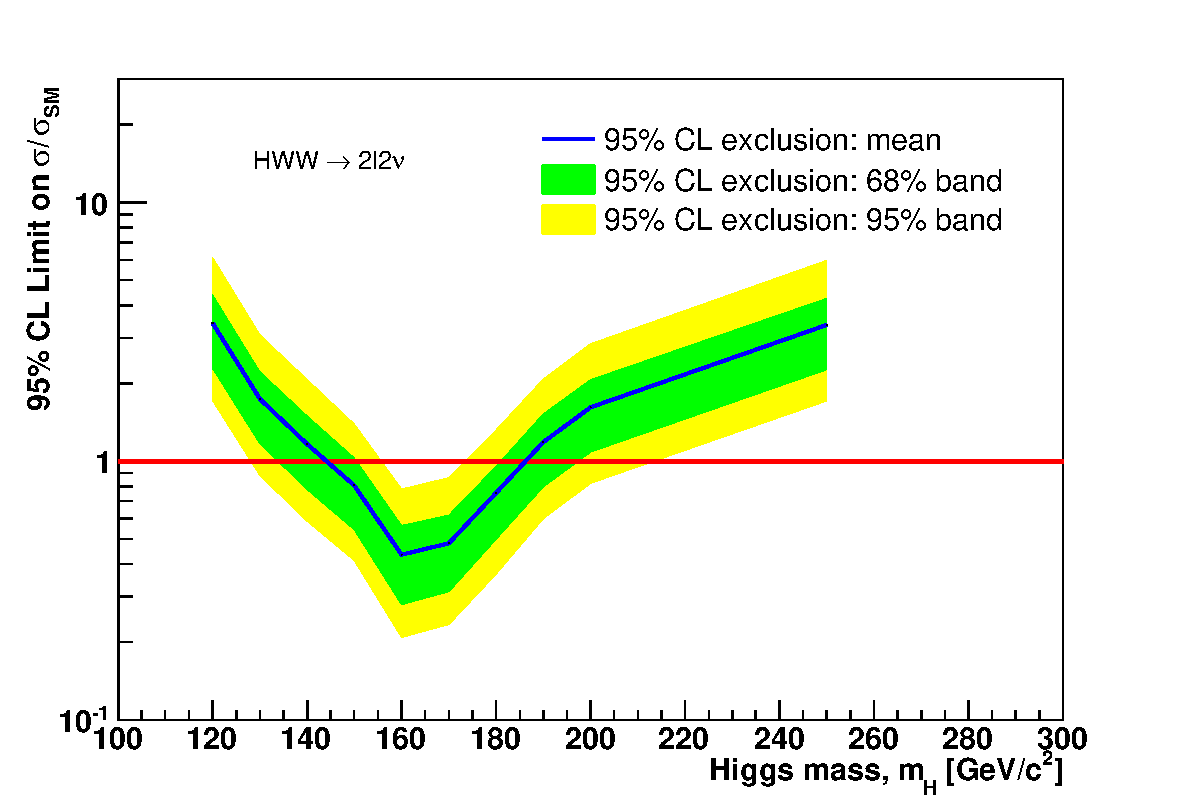
\includegraphics[width=0.9\textwidth]{figures/cut_based_limits.pdf}
   \caption{Cut based analysis expected upper limits at 95\%C.L. for 1\ifb\ of data.}
   \label{fig:cutbase_uls}
\end{center}
\end{figure}


\section{Summary}
     \label{sec:summary}
     In summary, we described an analysis to study the spin of a single narrow 
resonance at 125 GeV by the gluon fusion through the decays into $WW\to 2\ell2\nu$.  
The analysis is based on a two-dimensional templates $m_T-m_{\ell\ell}$. 
The expected sensitivity to distinguish between between SM Higgs hypothesis and 
spin 2 Graviton like resonance with minimal coupling 
$2_\text{min}^+$ is $1.7\sigma$ for \intlumiEightTeV. 
Scaling by luminosity the projected separation is about $2.0\sigma$ for 25~$\ifb$. 


%===================================================================================================
\clearpage

\vspace*{-0.2cm}
\thebibliography{12}

\bibitem{pdg}
 K. Nakamura et al. (Particle Data Group), "Review of particle physics", J. Phys.G37 , 2010.

\bibitem{Higgs1}
F. Englert and R. Brout, "Broken symmetries and the masses of gauge bosons", Phys. Rev. Lett. 13,  1964.

\bibitem{Higgs2}
P. W. Higgs, "Broken symmetry and the mass of gauge vector mesons", Phys. Rev. Lett. 13, 1964.

\bibitem{Higgs3}
Guralnik, G.S. and Hagen, C.R. and Kibble, T.W.B., "Global Conservation Laws and Massless Particles", 
Phys.Rev.Lett. 13, 1964.

\bibitem{HWW2010}
CMS Collaboration, "Title: Measurement of WW Production and Search for the Higgs Boson in 
pp Collisions at $\sqrt{s}$ = 7 TeV", arXiv:1102.5429

\bibitem{VBTFCrossSectionNote}
J. Alcaraz Maestre, \textit{et al.}, "Updated Measurements of Inclusive W and Z Cross Sections 
at $\sqrt{s}=7$ TeV", CMS AN-2010/264.

\bibitem{ggWWError}
F.~ Stoeckli, "http://indico.cern.ch/getFile.py/access?contribId=0\&resId=1\&materialId=slides\&confId=49009", 
EWK Diboson meeting of March 12 2009.

\bibitem{json}
{\small
/afs/cern.ch/cms/CAF/CMSCOMM/COMM\_DQM/certification/Collisions11/7TeV/Prompt/Cert\_160404-163869\_7TeV\_PromptReco\_Collisions11\_JSON.txt
}

\bibitem{ElIso}
A. Vartak, M. LeBourgeois, V. Sharma, "Lepton Isolation in the CMS Tracker, ECAL and HCAL", CMS AN-2010/106.

\bibitem{PVDA}
W. Erdmann, M. LeBourgeois, B. Mangano, 
https://indico.cern.ch/getFile.py/access?contribId=5\&sessionId=3\&resId=1\&materialId=slides\&confId=127127, 
note in preparation.

\bibitem{NExpHits}
B. Mangano \textit{et al.}, "Improvement in Photon Conversion Rejection Performance Using 
Advanced Tracking Tools", AN-10-283.

\bibitem{fakeLeptonNote1}
S.~Xie, \textit{et al.}", "Study of Data-Driven Methods for Estimation of Fake Lepton Backgrounds", 
CMS AN-2009/120.

\bibitem{fakeLeptonNote2}
W.~Andrews, \textit{et al.}, "Fake Rates for dilepton Analyses", CMS AN-2010/257.

\bibitem{fakeLeptonBkgSpillage1}
 F. Golf, D. Evans, J. Mulmenstadt  \textit{et al.}, ``Expectations for observation of top quark pair production in the dilepton final state with the early CMS data'', CMS AN-2009/050.

\bibitem{dyestnote}
W. Andrews, et al., “A Method to Measure the Contribution of $\dyll$ to a di-lepton+ MET Selection”, CMS AN-2009/023 (2009).

\bibitem{jes}
CMS Collaboration, "Jet Energy Calibration with Photon+Jet Events", PAS JME-09-004.

\bibitem{jetpas}
CMS Collaboration, "Jet Performance in pp Collisions at $\sqrt{s}=7 \rm\ TeV$", PAS JME-10-003.

\bibitem{btag}
CMS collaboration, "Commissioning of b-jet identification with pp collisions at $\sqrt{s}=7~\TeV$, BTV-10-001.

\bibitem{antikt}
Cacciari, Matteo and Salam, Gavin P. and Soyez, Gregory, "The anti-$k_t$ jet clustering 
algorithm", JHEP 04,  2008.

\bibitem{ConversionNote}
W.~Andrews, \textit{et al.}, "Study of photon conversion rejection at CMS", CMS AN-2009/159.

\bibitem{tmva}
A. Hoecker, \textit{et al.}, "TMVA - Toolkit for Multivariate Data Analysis", arXiv:physics/0703039, 2007.

\bibitem{XS}
CMS Generator group, Standard Model Cross Sections for CMS at 7 TeV, 2010.

\bibitem{PDF4LHC}
PDF4LHC Working Group, 
{\tt http://www.hep.ucl.ac.uk/pdf4lhc/PDF4LHCrecom.pdf}

\bibitem{Nadolsky:2008zw}
Nadolsky, Pavel M. and others, "Implications of CTEQ global analysis for 
collider observables", Phys. Rev. D78 2008.

\bibitem{Martin:2009iq}
Martin, A. D. and Stirling, W. J. and Thorne, R. S. and Watt, G., "Parton 
distributions for the LHC, Eur. Phys. J. C63 2009.

\bibitem{Ball:2010de}
Ball, Richard D. and others, "A first unbiased global NLO determination 
of parton distributions and their uncertainties", arXiv 1002.4407.

\bibitem{bayesian}
A. O'Hagan and J.J. Forster, "Bayesian Inference", Kendall's Advanced Theory of Statistics, 
Arnold, London, 2B, 2004.

\bibitem{ref:tagprobe_mit_w}
G. Bauer {\it et. al.}, "Lepton ef?iencies for the inclusive W cross section measurement with 36.1pb$^{-1}$", AN2011/097

\bibitem{ref:tagprobe_snt_top}
W. Andrews {\it et. al.}, "Uncertainties on the Lepton Selection Efficiency for t$t\bar{t}$ Cross Section Analysis", AN2010/274

\bibitem{LHCHiggsCrossSectionWorkingGroup:2011ti}
LHC Higgs Cross Section Working Group, "Handbook of LHC Higgs Cross Sections: 
Inclusive Observables", CERN-2011-002, 2011.

\bibitem{PFMET} 
CMS Collaboration, ``CMS MET Performance in Events Containing Electroweak Bosons from pp Collisions at $\sqrt{s}=7$ TeV'', CMS PAS JME-2010-005 (2010)


\bibitem{trkMET} 
Marco Zanetti, ``MET with PU in $\hww\to2\ell$'', https://indico.cern.ch/conferenceDisplay.py?confId=131580
Benjamin Hooberman, ``MET with PU in MC and First 2011 Data'', https://indico.cern.ch/contributionDisplay.py?contribId=5\&confId=132579. 


\bibitem{lands}
Mingshui Chen and Andrey Korytov, https://mschen.web.cern.ch/mschen/lands/

\bibitem{MCFMHiggsProduction}
J. Campbell, R.K. Ellis, G. Zanderighi, ``Next-to-Leading order Higgs + 2 jet production via gluon fusion.'', JHEP 0610:028 (2006), hep-ph/0608194
%===================================================================================================

\clearpage 
\appendix
\appendixpage

\section{ Details on $R_{out/in}$ for $\dyll$ Background Estimation}
     \label{app:appendix_dyr}
%     In this seciton, we document the details of estimation of the $R_{out/in}$, 
in support of Section~\ref{sec:bkg_dy}. 
Figure~\ref{fig:dyr_hww} shows the $R_{out/in}$ in the $ee$, $\mu\mu$ 
and $ee$/$\mu\mu$ final states at the WW preselection level in 
the 0/1/2 jet bins. 
Figure~\ref{fig:routin_0jet}-\ref{fig:routin_1jet} shows the $R_{out/in}$ in the 
$ee$/$\mu\mu$ final states at the Higgs selection level in the 
0 and 1 jet bins respectively. 

\begin{figure}[!hbtp]

\centering
\subfigure[ee 0-Jet]{
\centering
\label{subfig:dyr_ee_mh0_0j}
\includegraphics[width=.3\textwidth]{figures/Routin_ee_0Jet_mH0_5098pb_dy.pdf}}
\subfigure[$\mu\mu$ 0-Jet]{
\centering
\label{subfig:dyr_mm_mh0_0j}
\includegraphics[width=.3\textwidth]{figures/Routin_mm_0Jet_mH0_5098pb_dy.pdf}}
\subfigure[ee and $\mu\mu$ 0-Jet]{
\centering
\label{subfig:dyr_mh0_0j}
\includegraphics[width=.3\textwidth]{figures/Routin_0Jet_mH0_5098pb_dy.pdf}}
\centering
\subfigure[ee 1-Jet]{
\centering
\label{subfig:dyr_ee_mh0_1j}
\includegraphics[width=.3\textwidth]{figures/Routin_ee_1Jet_mH0_5098pb_dy.pdf}}
\subfigure[$\mu\mu$ 1-Jet]{
\centering
\label{subfig:dyr_mm_mh0_1j}
\includegraphics[width=.3\textwidth]{figures/Routin_mm_1Jet_mH0_5098pb_dy.pdf}}
\subfigure[ee and$\mu\mu$ 1-Jet]{
\centering
\label{subfig:dyr_mh0_1j}
\includegraphics[width=.3\textwidth]{figures/Routin_1Jet_mH0_5098pb_dy.pdf}}
\subfigure[ee 2-Jet]{
\centering
\label{subfig:dyr_ee_mh0_2j}
\includegraphics[width=.3\textwidth]{figures/Routin_ee_2Jet_mH0_5098pb_dy.pdf}}
\subfigure[$\mu\mu$ 2-Jet]{
\centering
\label{subfig:dyr_mm_mh0_2j}
\includegraphics[width=.3\textwidth]{figures/Routin_mm_2Jet_mH0_5098pb_dy.pdf}}
\subfigure[ee and $\mu\mu$ 2-Jet]{
\centering
\label{subfig:dyr_mh0_2j}
\includegraphics[width=.3\textwidth]{figures/Routin_2Jet_mH0_5098pb_dy.pdf}}
\caption{
 The \routin\, as a function of MET measured from data (black solid dots) 
and MC (red open circles) for the Drell-Yan processes after the WW preselections. 
The measurements in data are done using the opposite flavor subtraction method. }
\label{fig:dyr_hww}
\end{figure}

\begin{figure}[!htbp]
\begin{center}$
\begin{array}{cccc}
\includegraphics[width=.29\textwidth]{figures/Routin_0Jet_mH120_5098pb_dy.pdf} & 
\includegraphics[width=.29\textwidth]{figures/Routin_0Jet_mH125_5098pb_dy.pdf} & 
\includegraphics[width=.29\textwidth]{figures/Routin_0Jet_mH130_5098pb_dy.pdf} \\
\includegraphics[width=.29\textwidth]{figures/Routin_0Jet_mH135_5098pb_dy.pdf} & 
\includegraphics[width=.29\textwidth]{figures/Routin_0Jet_mH140_5098pb_dy.pdf} & 
\includegraphics[width=.29\textwidth]{figures/Routin_0Jet_mH150_5098pb_dy.pdf} \\
\includegraphics[width=.29\textwidth]{figures/Routin_0Jet_mH160_5098pb_dy.pdf} &
\includegraphics[width=.29\textwidth]{figures/Routin_0Jet_mH170_5098pb_dy.pdf} &
\includegraphics[width=.29\textwidth]{figures/Routin_0Jet_mH180_5098pb_dy.pdf} \\
\end{array}$
\caption{ The \routin\, (ee and $\mu\mu$ combined) as a function of MET measured from data (black solid dots) 
and MC (red open circles) for the Drell-Yan processes in the 0-Jet bin at the 
Higgs selection level in the cut-based analysis. 
The measurements in data are performed using the opposite flavor subtraction method. 
The difference in the \routin measurements in different higg selections are due to the 
different kinematic cuts applied. 
}
\label{fig:routin_0jet}
\end{center}
\end{figure}


\begin{figure}[!htbp]
\begin{center}$
\begin{array}{cccc}
\includegraphics[width=.29\textwidth]{figures/Routin_1Jet_mH120_5098pb_dy.pdf} & 
\includegraphics[width=.29\textwidth]{figures/Routin_1Jet_mH125_5098pb_dy.pdf} & 
\includegraphics[width=.29\textwidth]{figures/Routin_1Jet_mH130_5098pb_dy.pdf} \\
\includegraphics[width=.29\textwidth]{figures/Routin_1Jet_mH135_5098pb_dy.pdf} & 
\includegraphics[width=.29\textwidth]{figures/Routin_1Jet_mH140_5098pb_dy.pdf} & 
\includegraphics[width=.29\textwidth]{figures/Routin_1Jet_mH150_5098pb_dy.pdf} \\
\includegraphics[width=.29\textwidth]{figures/Routin_1Jet_mH160_5098pb_dy.pdf} &
\includegraphics[width=.29\textwidth]{figures/Routin_1Jet_mH170_5098pb_dy.pdf} &
\includegraphics[width=.29\textwidth]{figures/Routin_1Jet_mH180_5098pb_dy.pdf} \\
\end{array}$
\caption{ The \routin\, (ee and $\mu\mu$ combined) as a function of MET measured from data (black solid dots) 
and MC (red open circles) for the Drell-Yan processes in the 1-Jet bin at the 
Higgs selection level in the cut-based analysis. 
The measurements in data are performed using the opposite flavor subtraction method. 
The difference in the \routin measurements in different higg selections are due to the 
different kinematic cuts applied. 
}
\label{fig:routin_1jet}
\end{center}
\end{figure}

\clearpage

\section{\fixme Yield after Cut-based Selections with $\intlumiEightTeV$}
  \label{app:appendix_cutresults}
%  In this section, we document the details of the event yield after the Higgs 
selections in the cut-based analysis. 

\begin{table}
{%\footnotesize
 \tiny
 \begin{center}
 \begin{tabular}{l c c c c c c c c c c c }
 \hline
 process & ggH & qqWW & ggWW & VV & Top & Zjets & Wjets & Wgamma & Ztt & $\sum$Bkg & Data \\
 \hline
110 & $3.0\pm0.7$ & $44.5\pm5.6$ & $2.1\pm0.7$ & $1.1\pm0.1$ & $3.5\pm0.8$ & $0.1\pm0.0$ & $10.3\pm4.0$ & $9.3\pm4.3$ & $0.0\pm0.0$ & $71.1\pm8.3$ & 66 \\
115 & $6.2\pm1.4$ & $44.5\pm5.6$ & $2.1\pm0.7$ & $1.1\pm0.1$ & $3.5\pm0.8$ & $0.1\pm0.0$ & $10.3\pm4.0$ & $9.3\pm4.3$ & $0.0\pm0.0$ & $71.1\pm8.3$ & 66 \\
120 & $12.5\pm2.9$ & $62.8\pm7.9$ & $3.3\pm1.1$ & $1.4\pm0.1$ & $4.7\pm1.1$ & $0.1\pm0.0$ & $12.9\pm5.0$ & $9.4\pm4.3$ & $0.0\pm0.0$ & $94.5\pm10.4$ & 92 \\
130 & $30.9\pm7.0$ & $83.6\pm10.5$ & $4.5\pm1.5$ & $1.7\pm0.2$ & $5.9\pm1.3$ & $0.2\pm0.1$ & $14.7\pm5.6$ & $7.1\pm3.4$ & $0.1\pm0.0$ & $117.8\pm12.6$ & 117 \\
140 & $45.7\pm10.3$ & $83.4\pm10.4$ & $4.4\pm1.4$ & $1.4\pm0.2$ & $5.6\pm1.3$ & $0.2\pm0.0$ & $10.3\pm4.0$ & $6.0\pm3.2$ & $0.0\pm0.0$ & $111.4\pm11.8$ & 105 \\
150 & $48.2\pm11.1$ & $61.2\pm7.8$ & $4.5\pm1.5$ & $0.8\pm0.1$ & $5.2\pm1.2$ & $0.1\pm0.0$ & $4.8\pm2.0$ & $0.9\pm0.6$ & $0.0\pm0.0$ & $77.6\pm8.3$ & 83 \\
160 & $71.3\pm16.3$ & $41.9\pm5.4$ & $4.2\pm1.4$ & $0.6\pm0.1$ & $4.3\pm1.0$ & $0.0\pm0.0$ & $2.9\pm1.4$ & $0.7\pm0.5$ & $0.0\pm0.0$ & $54.6\pm5.9$ & 59 \\
170 & $55.5\pm12.9$ & $31.5\pm4.1$ & $4.1\pm1.4$ & $0.4\pm0.1$ & $3.9\pm0.9$ & $0.0\pm0.0$ & $2.8\pm1.4$ & $0.6\pm0.5$ & $0.0\pm0.0$ & $43.3\pm4.6$ & 46 \\
180 & $40.1\pm9.3$ & $36.5\pm4.7$ & $4.9\pm1.6$ & $0.5\pm0.1$ & $5.2\pm1.2$ & $0.0\pm0.0$ & $2.0\pm1.1$ & $0.6\pm0.5$ & $0.0\pm0.0$ & $49.7\pm5.3$ & 53 \\
190 & $34.5\pm8.2$ & $57.5\pm7.4$ & $6.9\pm2.2$ & $0.9\pm0.1$ & $9.6\pm2.1$ & $0.1\pm0.0$ & $2.3\pm1.1$ & $0.3\pm0.3$ & $0.0\pm0.0$ & $77.6\pm8.1$ & 72 \\
200 & $26.4\pm6.3$ & $56.8\pm10.6$ & $6.3\pm2.2$ & $1.0\pm0.1$ & $11.2\pm2.5$ & $0.1\pm0.0$ & $2.4\pm1.2$ & $0.2\pm0.2$ & $0.0\pm0.0$ & $78.0\pm11.1$ & 87 \\
250 & $15.0\pm3.8$ & $59.3\pm11.0$ & $5.3\pm1.9$ & $1.1\pm0.1$ & $19.3\pm4.2$ & $0.1\pm0.0$ & $4.3\pm1.8$ & $0.5\pm0.3$ & $0.0\pm0.0$ & $89.9\pm12.1$ & 93 \\
300 & $11.8\pm3.2$ & $50.9\pm9.5$ & $3.9\pm1.4$ & $1.0\pm0.1$ & $21.8\pm4.7$ & $0.1\pm0.0$ & $3.9\pm1.7$ & $1.2\pm0.6$ & $0.0\pm0.0$ & $82.7\pm10.8$ & 78 \\
350 & $12.4\pm3.7$ & $43.5\pm8.1$ & $3.1\pm1.1$ & $0.9\pm0.1$ & $21.3\pm4.6$ & $0.1\pm0.0$ & $4.0\pm1.8$ & $1.0\pm0.5$ & $0.0\pm0.0$ & $73.9\pm9.6$ & 72 \\
400 & $9.8\pm2.9$ & $34.2\pm6.4$ & $2.4\pm0.9$ & $0.7\pm0.1$ & $18.7\pm4.0$ & $0.1\pm0.0$ & $3.3\pm1.5$ & $0.9\pm0.5$ & $0.0\pm0.0$ & $60.3\pm7.8$ & 61 \\
450 & $5.7\pm1.9$ & $19.6\pm3.7$ & $1.5\pm0.5$ & $0.5\pm0.1$ & $11.8\pm2.6$ & $0.0\pm0.0$ & $1.7\pm0.8$ & $0.7\pm0.4$ & $0.0\pm0.0$ & $35.9\pm4.6$ & 37 \\
500 & $3.5\pm1.3$ & $14.8\pm2.8$ & $1.3\pm0.4$ & $0.4\pm0.1$ & $9.0\pm2.0$ & $0.0\pm0.0$ & $1.6\pm0.8$ & $0.6\pm0.4$ & $0.0\pm0.0$ & $27.6\pm3.6$ & 24 \\
550 & $2.2\pm1.0$ & $11.7\pm2.2$ & $1.1\pm0.4$ & $0.3\pm0.0$ & $6.8\pm1.5$ & $0.0\pm0.0$ & $1.4\pm0.7$ & $0.6\pm0.4$ & $0.0\pm0.0$ & $22.0\pm2.9$ & 20 \\
600 & $1.4\pm0.7$ & $9.6\pm1.8$ & $0.8\pm0.3$ & $0.2\pm0.0$ & $5.0\pm1.1$ & $0.0\pm0.0$ & $0.9\pm0.5$ & $0.5\pm0.4$ & $0.0\pm0.0$ & $17.1\pm2.3$ & 18 \\
\hline
\end{tabular}
\end{center}
}
\caption{Summary of the cut-based yields in the 0-Jet bin opposite flavor ($e\mu$) final states corresponding to \intlumi\ data.}
\end{table}
\begin{table}
{\tiny
 \tiny
 \begin{center}
 \begin{tabular}{l c c c c c c c c c c c }
 \hline
 process & ggH & qqWW & ggWW & VV & Top & Zjets & Wjets & Wgamma & Ztt & $\sum$Bkg & Data \\
 \hline
110 & $0.8\pm0.2$ & $21.4\pm2.8$ & $0.8\pm0.3$ & $0.4\pm0.1$ & $1.0\pm0.3$ & $8.5\pm6.4$ & $2.4\pm1.2$ & $0.2\pm0.2$ & $0.0\pm0.0$ & $34.8\pm7.1$ & 29 \\
115 & $1.9\pm0.5$ & $21.4\pm2.8$ & $0.8\pm0.3$ & $0.4\pm0.1$ & $1.0\pm0.3$ & $8.5\pm6.4$ & $2.4\pm1.2$ & $0.2\pm0.2$ & $0.0\pm0.0$ & $34.8\pm7.1$ & 29 \\
120 & $4.9\pm1.1$ & $35.9\pm4.6$ & $1.5\pm0.5$ & $0.6\pm0.1$ & $2.1\pm0.6$ & $10.4\pm7.7$ & $3.3\pm1.5$ & $0.3\pm0.2$ & $0.0\pm0.0$ & $54.1\pm9.1$ & 49 \\
130 & $16.0\pm3.6$ & $54.4\pm6.9$ & $2.5\pm0.8$ & $0.9\pm0.1$ & $3.1\pm0.8$ & $13.2\pm9.2$ & $4.5\pm1.9$ & $0.3\pm0.2$ & $0.0\pm0.0$ & $78.9\pm11.7$ & 80 \\
140 & $29.1\pm6.6$ & $62.6\pm7.9$ & $3.0\pm1.0$ & $1.0\pm0.1$ & $3.6\pm0.9$ & $14.6\pm10.1$ & $4.9\pm2.1$ & $0.3\pm0.2$ & $0.0\pm0.0$ & $89.9\pm13.0$ & 89 \\
150 & $36.7\pm8.4$ & $49.9\pm6.4$ & $3.3\pm1.1$ & $0.7\pm0.1$ & $4.1\pm1.0$ & $7.1\pm6.8$ & $1.8\pm1.0$ & $0.8\pm0.7$ & $0.0\pm0.0$ & $67.8\pm9.5$ & 82 \\
160 & $55.0\pm12.6$ & $35.3\pm4.6$ & $3.1\pm1.0$ & $0.4\pm0.1$ & $4.0\pm1.0$ & $4.2\pm7.0$ & $0.6\pm0.6$ & $0.0\pm0.0$ & $0.0\pm0.0$ & $47.7\pm8.5$ & 50 \\
170 & $45.9\pm10.7$ & $29.0\pm3.8$ & $3.0\pm1.0$ & $0.4\pm0.1$ & $3.9\pm1.0$ & $2.0\pm3.1$ & $0.5\pm0.5$ & $0.1\pm0.1$ & $0.0\pm0.0$ & $38.9\pm5.1$ & 41 \\
180 & $37.2\pm8.7$ & $34.4\pm4.4$ & $3.9\pm1.3$ & $0.5\pm0.1$ & $4.6\pm1.1$ & $1.4\pm1.6$ & $0.3\pm0.5$ & $0.4\pm0.3$ & $0.0\pm0.0$ & $45.5\pm5.0$ & 43 \\
190 & $32.4\pm7.7$ & $53.3\pm6.9$ & $5.5\pm1.8$ & $0.8\pm0.1$ & $6.9\pm1.5$ & $3.6\pm3.5$ & $1.1\pm0.9$ & $0.4\pm0.3$ & $0.0\pm0.0$ & $71.6\pm8.1$ & 73 \\
200 & $21.5\pm5.1$ & $45.2\pm8.4$ & $4.8\pm1.7$ & $0.8\pm0.1$ & $7.1\pm1.6$ & $3.8\pm2.6$ & $1.6\pm1.0$ & $0.4\pm0.3$ & $0.0\pm0.0$ & $63.6\pm9.2$ & 71 \\
250 & $8.3\pm2.1$ & $36.2\pm6.8$ & $3.2\pm1.1$ & $0.6\pm0.1$ & $11.0\pm2.4$ & $3.7\pm0.5$ & $2.4\pm1.2$ & $0.2\pm0.2$ & $0.0\pm0.0$ & $57.3\pm7.4$ & 61 \\
300 & $8.2\pm2.2$ & $35.0\pm6.5$ & $2.4\pm0.9$ & $0.6\pm0.1$ & $13.7\pm3.0$ & $3.8\pm0.8$ & $2.0\pm0.9$ & $0.6\pm0.4$ & $0.0\pm0.0$ & $58.0\pm7.3$ & 70 \\
350 & $9.5\pm2.9$ & $31.1\pm5.8$ & $2.2\pm0.8$ & $0.6\pm0.1$ & $13.8\pm3.0$ & $4.6\pm1.4$ & $2.6\pm1.2$ & $2.1\pm0.9$ & $0.0\pm0.0$ & $56.9\pm6.9$ & 63 \\
400 & $7.6\pm2.2$ & $25.6\pm4.8$ & $1.9\pm0.7$ & $0.5\pm0.1$ & $11.7\pm2.5$ & $2.9\pm0.3$ & $2.5\pm1.1$ & $2.1\pm0.9$ & $0.0\pm0.0$ & $47.2\pm5.7$ & 49 \\
450 & $4.3\pm1.4$ & $13.7\pm2.6$ & $1.4\pm0.5$ & $0.3\pm0.0$ & $8.0\pm1.8$ & $1.8\pm0.2$ & $1.9\pm0.9$ & $1.1\pm0.6$ & $0.0\pm0.0$ & $28.3\pm3.4$ & 29 \\
500 & $2.6\pm1.0$ & $9.8\pm1.9$ & $1.2\pm0.4$ & $0.2\pm0.0$ & $6.2\pm1.4$ & $1.5\pm0.2$ & $1.5\pm0.8$ & $0.6\pm0.4$ & $0.0\pm0.0$ & $21.1\pm2.5$ & 24 \\
550 & $1.6\pm0.7$ & $7.2\pm1.4$ & $0.8\pm0.3$ & $0.2\pm0.0$ & $4.5\pm1.0$ & $1.2\pm0.2$ & $1.4\pm0.7$ & $0.4\pm0.3$ & $0.0\pm0.0$ & $15.6\pm1.9$ & 22 \\
600 & $1.0\pm0.5$ & $5.9\pm1.2$ & $0.7\pm0.3$ & $0.1\pm0.0$ & $3.5\pm0.8$ & $0.9\pm0.1$ & $1.1\pm0.6$ & $0.0\pm0.0$ & $0.0\pm0.0$ & $12.2\pm1.6$ & 15 \\
\hline
\end{tabular}
\end{center}
}
\caption{Summary of the cut-based yields in the 0-Jet bin same flavor (ee and $\mu\mu$) final states corresponding to \intlumi\ data.}
\end{table}
\begin{table}
{%\footnotesize
 \tiny
 \begin{center}
 \begin{tabular}{l c c c c c c c c c c c }
 \hline
 process & ggH & qqWW & ggWW & VV & Top & Zjets & Wjets & Wgamma & Ztt & $\sum$Bkg & Data \\
 \hline
110 & $1.4\pm0.5$ & $14.5\pm2.5$ & $0.7\pm0.3$ & $1.6\pm0.2$ & $9.3\pm0.8$ & $0.1\pm0.0$ & $7.4\pm3.0$ & $1.6\pm0.7$ & $0.1\pm0.0$ & $35.3\pm4.1$ & 48 \\
115 & $2.6\pm0.9$ & $14.5\pm2.5$ & $0.7\pm0.3$ & $1.6\pm0.2$ & $9.3\pm0.8$ & $0.1\pm0.0$ & $7.4\pm3.0$ & $1.6\pm0.7$ & $0.1\pm0.0$ & $35.3\pm4.1$ & 48 \\
120 & $5.0\pm1.7$ & $19.6\pm3.4$ & $1.1\pm0.4$ & $1.9\pm0.2$ & $12.7\pm1.0$ & $0.2\pm0.0$ & $8.7\pm3.5$ & $1.8\pm0.8$ & $0.1\pm0.0$ & $46.0\pm5.1$ & 57 \\
130 & $12.2\pm4.2$ & $26.0\pm4.5$ & $1.5\pm0.5$ & $2.3\pm0.3$ & $17.1\pm1.2$ & $0.3\pm0.1$ & $8.9\pm3.5$ & $1.5\pm0.7$ & $0.1\pm0.0$ & $57.7\pm5.9$ & 73 \\
140 & $18.1\pm6.0$ & $25.8\pm4.4$ & $1.5\pm0.5$ & $2.0\pm0.2$ & $16.0\pm1.2$ & $0.3\pm0.1$ & $5.6\pm2.3$ & $1.3\pm0.7$ & $0.0\pm0.0$ & $52.4\pm5.2$ & 58 \\
150 & $20.5\pm6.7$ & $23.6\pm4.1$ & $1.8\pm0.6$ & $1.4\pm0.2$ & $16.8\pm1.2$ & $0.1\pm0.0$ & $2.2\pm1.1$ & $0.8\pm0.5$ & $0.0\pm0.0$ & $46.8\pm4.5$ & 44 \\
160 & $31.5\pm10.3$ & $19.9\pm3.5$ & $1.6\pm0.6$ & $1.1\pm0.1$ & $14.0\pm1.1$ & $0.1\pm0.0$ & $1.9\pm1.0$ & $0.2\pm0.2$ & $0.0\pm0.0$ & $38.8\pm3.8$ & 32 \\
170 & $24.8\pm8.0$ & $15.9\pm2.8$ & $1.5\pm0.5$ & $0.6\pm0.1$ & $11.5\pm0.9$ & $0.1\pm0.0$ & $1.1\pm0.7$ & $0.2\pm0.2$ & $0.0\pm0.0$ & $30.8\pm3.0$ & 21 \\
180 & $19.1\pm6.1$ & $18.7\pm3.3$ & $1.9\pm0.7$ & $0.5\pm0.1$ & $14.6\pm1.1$ & $0.1\pm0.0$ & $0.9\pm0.7$ & $0.0\pm0.0$ & $0.0\pm0.0$ & $36.7\pm3.6$ & 26 \\
190 & $17.3\pm5.6$ & $30.7\pm5.3$ & $2.7\pm1.0$ & $0.9\pm0.1$ & $25.8\pm1.8$ & $0.2\pm0.0$ & $1.5\pm1.0$ & $0.0\pm0.0$ & $0.0\pm0.0$ & $61.9\pm5.7$ & 39 \\
200 & $13.2\pm4.1$ & $29.0\pm6.4$ & $2.5\pm0.9$ & $1.1\pm0.1$ & $30.9\pm2.1$ & $0.2\pm0.0$ & $2.2\pm1.2$ & $0.0\pm0.0$ & $0.0\pm0.0$ & $65.9\pm6.9$ & 48 \\
250 & $8.7\pm2.7$ & $37.4\pm8.3$ & $2.5\pm0.9$ & $1.6\pm0.2$ & $48.9\pm3.2$ & $0.2\pm0.0$ & $3.6\pm1.6$ & $0.0\pm0.0$ & $0.1\pm0.0$ & $94.2\pm9.1$ & 84 \\
300 & $7.1\pm2.2$ & $35.7\pm7.9$ & $2.0\pm0.7$ & $1.5\pm0.2$ & $47.5\pm3.1$ & $0.2\pm0.0$ & $4.7\pm2.0$ & $0.3\pm0.2$ & $0.1\pm0.0$ & $91.9\pm8.7$ & 87 \\
350 & $8.0\pm2.6$ & $32.3\pm7.2$ & $1.6\pm0.6$ & $1.3\pm0.2$ & $42.4\pm2.8$ & $0.1\pm0.0$ & $4.2\pm1.8$ & $0.5\pm0.4$ & $0.1\pm0.0$ & $82.6\pm7.9$ & 75 \\
400 & $6.8\pm2.2$ & $27.6\pm6.1$ & $1.5\pm0.5$ & $1.1\pm0.1$ & $35.3\pm2.4$ & $0.1\pm0.0$ & $4.4\pm1.9$ & $0.5\pm0.4$ & $0.1\pm0.0$ & $70.5\pm6.9$ & 62 \\
450 & $4.1\pm1.4$ & $18.5\pm4.1$ & $1.0\pm0.4$ & $0.7\pm0.1$ & $21.5\pm1.5$ & $0.1\pm0.0$ & $3.1\pm1.4$ & $0.5\pm0.4$ & $0.0\pm0.0$ & $45.5\pm4.6$ & 35 \\
500 & $2.8\pm1.0$ & $15.4\pm3.4$ & $0.8\pm0.3$ & $0.6\pm0.1$ & $17.2\pm1.3$ & $0.1\pm0.0$ & $2.7\pm1.2$ & $0.5\pm0.4$ & $0.0\pm0.0$ & $37.3\pm3.9$ & 30 \\
550 & $1.9\pm0.8$ & $12.5\pm2.8$ & $0.7\pm0.2$ & $0.5\pm0.1$ & $13.7\pm1.0$ & $0.1\pm0.0$ & $2.6\pm1.2$ & $0.5\pm0.4$ & $0.0\pm0.0$ & $30.5\pm3.3$ & 24 \\
600 & $1.2\pm0.5$ & $10.6\pm2.4$ & $0.5\pm0.2$ & $0.4\pm0.1$ & $10.6\pm0.8$ & $0.1\pm0.0$ & $2.1\pm1.0$ & $0.2\pm0.3$ & $0.0\pm0.0$ & $24.6\pm2.8$ & 20 \\
\hline
\end{tabular}
\end{center}
}
\caption{Summary of the cut-based yields in the 1-Jet bin opposite flavor ($e\mu$) final states corresponding to \intlumi\ data.}
\end{table}
\begin{table}
{%\footnotesize
 \tiny
 \begin{center}
 \begin{tabular}{l c c c c c c c c c c c }
 \hline
 process & ggH & qqWW & ggWW & VV & Top & Zjets & Wjets & Wgamma & Ztt & $\sum$Bkg & Data \\
 \hline
110 & $0.3\pm0.1$ & $4.9\pm0.9$ & $0.2\pm0.1$ & $0.3\pm0.1$ & $3.1\pm0.3$ & $5.8\pm3.1$ & $0.6\pm0.4$ & $0.0\pm0.0$ & $0.0\pm0.0$ & $14.9\pm3.3$ & 15 \\
115 & $0.7\pm0.2$ & $4.9\pm0.9$ & $0.2\pm0.1$ & $0.3\pm0.1$ & $3.1\pm0.3$ & $5.8\pm3.1$ & $0.6\pm0.4$ & $0.0\pm0.0$ & $0.0\pm0.0$ & $14.9\pm3.3$ & 15 \\
120 & $1.4\pm0.5$ & $7.7\pm1.4$ & $0.4\pm0.1$ & $0.5\pm0.1$ & $5.2\pm0.5$ & $9.9\pm5.4$ & $0.9\pm0.5$ & $0.0\pm0.0$ & $0.0\pm0.0$ & $24.6\pm5.6$ & 27 \\
130 & $4.9\pm1.7$ & $12.6\pm2.2$ & $0.8\pm0.3$ & $0.7\pm0.1$ & $7.8\pm0.7$ & $9.0\pm5.1$ & $2.3\pm1.1$ & $0.8\pm0.8$ & $0.0\pm0.0$ & $33.9\pm5.8$ & 41 \\
140 & $9.4\pm3.1$ & $14.9\pm2.6$ & $0.9\pm0.3$ & $0.8\pm0.1$ & $9.2\pm0.7$ & $12.4\pm6.8$ & $2.4\pm1.2$ & $0.8\pm0.8$ & $0.0\pm0.0$ & $41.4\pm7.5$ & 47 \\
150 & $13.5\pm4.4$ & $15.8\pm2.8$ & $1.3\pm0.5$ & $0.6\pm0.1$ & $10.8\pm0.8$ & $12.6\pm6.2$ & $2.5\pm1.3$ & $0.8\pm0.8$ & $0.0\pm0.0$ & $44.3\pm7.0$ & 51 \\
160 & $22.4\pm7.3$ & $13.1\pm2.3$ & $1.2\pm0.4$ & $0.5\pm0.1$ & $10.0\pm0.8$ & $10.8\pm5.7$ & $1.8\pm1.1$ & $0.0\pm0.0$ & $0.0\pm0.0$ & $37.4\pm6.3$ & 52 \\
170 & $18.4\pm6.0$ & $11.8\pm2.1$ & $1.2\pm0.4$ & $0.4\pm0.1$ & $9.3\pm0.8$ & $10.8\pm6.7$ & $1.8\pm1.1$ & $0.0\pm0.0$ & $0.0\pm0.0$ & $35.3\pm7.2$ & 44 \\
180 & $15.6\pm5.0$ & $14.7\pm2.6$ & $1.4\pm0.5$ & $0.4\pm0.1$ & $12.6\pm1.0$ & $8.9\pm5.7$ & $2.4\pm1.3$ & $0.9\pm1.0$ & $0.0\pm0.0$ & $41.3\pm6.6$ & 40 \\
190 & $12.4\pm4.0$ & $22.4\pm3.9$ & $2.0\pm0.7$ & $0.6\pm0.1$ & $19.8\pm1.4$ & $12.7\pm6.9$ & $2.4\pm1.3$ & $1.8\pm1.4$ & $0.0\pm0.0$ & $61.5\pm8.3$ & 54 \\
200 & $9.4\pm2.9$ & $18.6\pm4.1$ & $1.6\pm0.6$ & $0.6\pm0.1$ & $21.0\pm1.5$ & $12.3\pm6.3$ & $2.5\pm1.4$ & $1.8\pm1.4$ & $0.0\pm0.0$ & $58.5\pm8.0$ & 61 \\
250 & $4.2\pm1.3$ & $21.4\pm4.8$ & $1.1\pm0.4$ & $0.8\pm0.1$ & $25.8\pm1.8$ & $8.8\pm3.1$ & $2.1\pm1.2$ & $1.0\pm1.0$ & $0.0\pm0.0$ & $60.9\pm6.2$ & 71 \\
300 & $4.6\pm1.5$ & $20.2\pm4.5$ & $1.1\pm0.4$ & $0.8\pm0.1$ & $26.4\pm1.8$ & $7.6\pm3.1$ & $2.1\pm1.1$ & $1.7\pm1.7$ & $0.0\pm0.0$ & $59.9\pm6.1$ & 80 \\
350 & $5.2\pm1.7$ & $19.4\pm4.3$ & $1.0\pm0.3$ & $0.8\pm0.1$ & $23.4\pm1.6$ & $5.7\pm2.1$ & $1.9\pm0.9$ & $2.0\pm1.7$ & $0.0\pm0.0$ & $54.1\pm5.4$ & 74 \\
400 & $4.8\pm1.6$ & $16.5\pm3.7$ & $0.8\pm0.3$ & $0.6\pm0.1$ & $20.1\pm1.4$ & $4.3\pm1.6$ & $2.0\pm0.9$ & $2.0\pm1.7$ & $0.0\pm0.0$ & $46.2\pm4.7$ & 66 \\
450 & $2.8\pm1.0$ & $10.8\pm2.4$ & $0.6\pm0.2$ & $0.4\pm0.1$ & $12.5\pm0.9$ & $1.1\pm0.2$ & $1.8\pm0.8$ & $0.2\pm0.2$ & $0.0\pm0.0$ & $27.4\pm2.8$ & 40 \\
500 & $1.9\pm0.7$ & $8.6\pm2.0$ & $0.4\pm0.2$ & $0.3\pm0.0$ & $9.9\pm0.8$ & $1.0\pm0.2$ & $1.5\pm0.7$ & $0.2\pm0.2$ & $0.0\pm0.0$ & $21.9\pm2.3$ & 32 \\
550 & $1.2\pm0.5$ & $6.7\pm1.5$ & $0.4\pm0.1$ & $0.2\pm0.0$ & $7.3\pm0.6$ & $0.8\pm0.2$ & $1.5\pm0.7$ & $0.2\pm0.2$ & $0.0\pm0.0$ & $17.1\pm1.8$ & 22 \\
600 & $0.8\pm0.3$ & $5.3\pm1.2$ & $0.3\pm0.1$ & $0.2\pm0.0$ & $5.5\pm0.5$ & $0.7\pm0.2$ & $1.2\pm0.6$ & $0.2\pm0.2$ & $0.0\pm0.0$ & $13.4\pm1.5$ & 16 \\
\hline
\end{tabular}
\end{center}
}
\caption{Summary of the cut-based yields in the 1-Jet bin same flavor (ee and $\mu\mu$) final states corresponding to \intlumi\ data.}
\end{table}
\begin{table}
{%\footnotesize
 \tiny
 \begin{center}
 \begin{tabular}{l c c c c c c c c c c c }
 \hline
 process & ggH & qqWW & ggWW & VV & Top & Zjets & Wjets & Wgamma & Ztt & $\sum$Bkg & Data \\
 \hline
110 & $0.0\pm0.0$ & $1.7\pm0.8$ & $0.3\pm0.1$ & $0.1\pm0.0$ & $3.4\pm0.9$ & $4.0\pm4.2$ & $0.6\pm0.5$ & $0.4\pm0.3$ & $0.2\pm0.1$ & $10.7\pm4.4$ & 7 \\
115 & $0.1\pm0.0$ & $1.7\pm0.8$ & $0.3\pm0.1$ & $0.1\pm0.0$ & $3.4\pm0.9$ & $4.0\pm4.2$ & $0.6\pm0.5$ & $0.4\pm0.3$ & $0.2\pm0.1$ & $10.7\pm4.4$ & 7 \\
120 & $0.2\pm0.1$ & $1.7\pm0.8$ & $0.3\pm0.1$ & $0.1\pm0.0$ & $3.4\pm0.9$ & $4.0\pm4.2$ & $0.6\pm0.5$ & $0.4\pm0.3$ & $0.2\pm0.1$ & $10.7\pm4.4$ & 7 \\
130 & $0.6\pm0.2$ & $2.0\pm1.0$ & $0.3\pm0.1$ & $0.1\pm0.0$ & $4.1\pm1.1$ & $4.0\pm4.2$ & $0.6\pm0.5$ & $0.4\pm0.3$ & $0.2\pm0.1$ & $11.8\pm4.5$ & 9 \\
140 & $1.0\pm0.3$ & $2.2\pm1.1$ & $0.4\pm0.1$ & $0.1\pm0.0$ & $4.6\pm1.2$ & $4.0\pm4.2$ & $0.8\pm0.6$ & $0.4\pm0.3$ & $0.2\pm0.1$ & $12.8\pm4.5$ & 10 \\
150 & $1.6\pm0.4$ & $2.4\pm1.1$ & $0.4\pm0.2$ & $0.1\pm0.0$ & $4.9\pm1.3$ & $4.0\pm4.4$ & $0.8\pm0.6$ & $0.4\pm0.3$ & $0.2\pm0.1$ & $13.4\pm4.8$ & 11 \\
160 & $2.0\pm0.6$ & $2.4\pm1.1$ & $0.4\pm0.2$ & $0.1\pm0.0$ & $4.9\pm1.3$ & $4.0\pm4.4$ & $0.8\pm0.6$ & $0.4\pm0.3$ & $0.2\pm0.1$ & $13.4\pm4.8$ & 11 \\
170 & $2.7\pm0.8$ & $2.4\pm1.2$ & $0.4\pm0.2$ & $0.1\pm0.0$ & $4.9\pm1.3$ & $4.0\pm4.4$ & $0.8\pm0.6$ & $0.4\pm0.3$ & $0.2\pm0.1$ & $13.4\pm4.8$ & 11 \\
180 & $2.4\pm0.6$ & $2.4\pm1.1$ & $0.4\pm0.2$ & $0.1\pm0.0$ & $4.9\pm1.3$ & $4.0\pm4.4$ & $0.8\pm0.6$ & $0.4\pm0.3$ & $0.2\pm0.1$ & $13.4\pm4.7$ & 11 \\
190 & $1.7\pm0.4$ & $2.4\pm1.1$ & $0.4\pm0.2$ & $0.1\pm0.0$ & $4.9\pm1.3$ & $4.0\pm4.3$ & $0.8\pm0.6$ & $0.4\pm0.3$ & $0.2\pm0.1$ & $13.4\pm4.6$ & 11 \\
200 & $1.3\pm0.4$ & $1.9\pm0.9$ & $0.3\pm0.1$ & $0.1\pm0.0$ & $4.9\pm1.3$ & $4.0\pm4.2$ & $0.8\pm0.6$ & $0.4\pm0.3$ & $0.2\pm0.1$ & $12.8\pm4.6$ & 11 \\
250 & $1.0\pm0.2$ & $3.1\pm1.5$ & $0.5\pm0.2$ & $0.2\pm0.0$ & $8.9\pm2.3$ & $5.7\pm6.0$ & $0.8\pm0.6$ & $0.4\pm0.3$ & $0.2\pm0.1$ & $19.8\pm6.7$ & 17 \\
300 & $0.8\pm0.2$ & $3.2\pm1.5$ & $0.5\pm0.2$ & $0.2\pm0.0$ & $9.1\pm2.3$ & $5.7\pm5.0$ & $0.8\pm0.6$ & $0.4\pm0.3$ & $0.2\pm0.1$ & $20.1\pm5.8$ & 18 \\
350 & $0.9\pm0.3$ & $3.2\pm1.5$ & $0.5\pm0.2$ & $0.2\pm0.0$ & $9.3\pm2.4$ & $5.7\pm4.4$ & $0.8\pm0.6$ & $0.4\pm0.3$ & $0.2\pm0.1$ & $20.3\pm5.3$ & 18 \\
400 & $0.8\pm0.2$ & $3.2\pm1.5$ & $0.5\pm0.2$ & $0.2\pm0.0$ & $9.3\pm2.4$ & $5.7\pm4.4$ & $0.8\pm0.6$ & $0.4\pm0.3$ & $0.2\pm0.1$ & $20.4\pm5.3$ & 18 \\
450 & $0.6\pm0.2$ & $3.2\pm1.5$ & $0.5\pm0.2$ & $0.2\pm0.0$ & $9.4\pm2.4$ & $5.7\pm4.5$ & $0.8\pm0.6$ & $0.4\pm0.3$ & $0.2\pm0.1$ & $20.5\pm5.3$ & 18 \\
500 & $0.4\pm0.1$ & $3.2\pm1.5$ & $0.5\pm0.2$ & $0.2\pm0.0$ & $9.4\pm2.4$ & $5.7\pm4.5$ & $0.8\pm0.6$ & $0.4\pm0.3$ & $0.2\pm0.1$ & $20.5\pm5.3$ & 18 \\
550 & $0.2\pm0.1$ & $3.2\pm1.5$ & $0.5\pm0.2$ & $0.2\pm0.0$ & $9.4\pm2.4$ & $5.7\pm4.4$ & $0.8\pm0.6$ & $0.4\pm0.3$ & $0.2\pm0.1$ & $20.5\pm5.3$ & 18 \\
600 & $0.2\pm0.1$ & $3.2\pm1.5$ & $0.5\pm0.2$ & $0.2\pm0.0$ & $9.5\pm2.4$ & $5.7\pm4.4$ & $0.8\pm0.6$ & $0.4\pm0.3$ & $0.2\pm0.1$ & $20.5\pm5.3$ & 18 \\
\hline
\end{tabular}
\end{center}
}
\caption{Summary of the cut-based yields in the 2-Jet bin final state corresponding to \intlumi\ data.}
\end{table}
\clearpage

\section{\fixme Yields after MVA Selections with $\intlumiEightTeV$}
   \label{app:appendix_bdtresults}
%   In this section, we document the details of the event yield in 
the multivariate based analysis.

\begin{table}
{%\footnotesize
 \tiny
 \begin{center}
 \begin{tabular}{l | c c | c c c c c c c c  | c c}
 \hline
 process & qqH & ggH & qqWW & ggWW & VV & Top & Zjets & Wjets & Wgamma & Ztt & $\sum$Bkg & Data \\
 \hline
110 & $0.0\pm0.0$ & $1.9\pm0.4$ & $58.4\pm7.3$ & $3.3\pm1.1$ & $1.7\pm0.1$ & $5.8\pm1.3$ & $0.2\pm0.0$ & $15.9\pm5.7$ & $3.4\pm1.3$ & $0.0\pm0.0$ & $88.7\pm9.5$ & N/A \\
115 & $0.0\pm0.0$ & $4.4\pm0.9$ & $73.3\pm9.1$ & $4.1\pm1.3$ & $2.0\pm0.1$ & $6.4\pm1.5$ & $0.2\pm0.0$ & $16.8\pm6.0$ & $3.6\pm1.3$ & $0.0\pm0.0$ & $106.3\pm11.2$ & N/A \\
120 & $0.0\pm0.0$ & $8.9\pm1.8$ & $87.0\pm10.8$ & $5.0\pm1.6$ & $2.3\pm0.1$ & $7.1\pm1.6$ & $0.2\pm0.0$ & $18.7\pm6.7$ & $3.8\pm1.4$ & $0.0\pm0.0$ & $124.1\pm13.0$ & N/A \\
125 & $0.2\pm0.0$ & $16.4\pm3.3$ & $116.5\pm14.5$ & $6.5\pm2.1$ & $3.0\pm0.2$ & $9.3\pm2.1$ & $0.4\pm0.0$ & $23.0\pm8.3$ & $3.9\pm1.4$ & $0.0\pm0.0$ & $162.6\pm17.0$ & N/A \\
130 & $0.3\pm0.0$ & $25.5\pm5.1$ & $131.1\pm16.3$ & $7.9\pm2.5$ & $3.2\pm0.2$ & $10.0\pm2.3$ & $0.4\pm0.0$ & $23.5\pm8.4$ & $3.9\pm1.4$ & $0.0\pm0.0$ & $179.9\pm18.7$ & N/A \\
135 & $0.0\pm0.0$ & $36.6\pm7.3$ & $163.7\pm20.3$ & $9.7\pm3.1$ & $3.9\pm0.2$ & $13.4\pm3.1$ & $0.4\pm0.0$ & $26.2\pm9.4$ & $4.6\pm1.7$ & $0.0\pm0.0$ & $221.9\pm22.9$ & N/A \\
140 & $0.8\pm0.0$ & $48.8\pm9.8$ & $176.4\pm21.9$ & $10.8\pm3.4$ & $4.1\pm0.2$ & $14.7\pm3.4$ & $0.5\pm0.0$ & $27.5\pm9.9$ & $4.7\pm1.7$ & $0.0\pm0.0$ & $238.6\pm24.6$ & N/A \\
145 & $0.9\pm0.1$ & $62.1\pm12.4$ & $167.4\pm21.1$ & $10.6\pm3.4$ & $4.3\pm0.3$ & $16.1\pm3.7$ & $0.5\pm0.0$ & $26.9\pm9.7$ & $4.7\pm1.7$ & $0.0\pm0.0$ & $230.7\pm23.8$ & N/A \\
150 & $1.2\pm0.1$ & $78.3\pm16.0$ & $193.1\pm24.3$ & $12.4\pm4.0$ & $5.0\pm0.3$ & $20.4\pm4.6$ & $0.5\pm0.0$ & $30.1\pm10.8$ & $4.8\pm1.7$ & $0.0\pm0.0$ & $266.3\pm27.3$ & N/A \\
160 & $1.9\pm0.1$ & $111.9\pm22.9$ & $206.5\pm26.0$ & $14.1\pm4.5$ & $5.2\pm0.3$ & $23.5\pm5.4$ & $0.5\pm0.1$ & $30.7\pm11.1$ & $5.2\pm1.9$ & $0.0\pm0.0$ & $285.7\pm29.1$ & N/A \\
170 & $2.1\pm0.1$ & $109.7\pm23.0$ & $214.5\pm27.0$ & $15.2\pm4.9$ & $5.4\pm0.3$ & $26.3\pm6.0$ & $0.5\pm0.1$ & $31.7\pm11.4$ & $5.4\pm1.9$ & $0.0\pm0.0$ & $299.1\pm30.4$ & N/A \\
180 & $0.0\pm0.0$ & $94.6\pm19.8$ & $245.2\pm31.2$ & $17.4\pm5.6$ & $5.9\pm0.4$ & $29.3\pm6.7$ & $0.5\pm0.1$ & $32.8\pm11.8$ & $5.6\pm2.0$ & $0.0\pm0.0$ & $336.8\pm34.6$ & N/A \\
190 & $1.5\pm0.1$ & $68.0\pm14.6$ & $257.4\pm34.7$ & $18.2\pm5.9$ & $6.4\pm0.4$ & $32.7\pm7.5$ & $0.6\pm0.1$ & $33.1\pm11.9$ & $5.8\pm2.0$ & $0.0\pm0.0$ & $354.2\pm38.0$ & N/A \\
200 & $1.2\pm0.1$ & $57.1\pm12.2$ & $240.5\pm20.8$ & $16.9\pm5.1$ & $6.8\pm0.4$ & $37.6\pm8.6$ & $0.6\pm0.1$ & $33.9\pm12.2$ & $6.1\pm2.1$ & $0.0\pm0.0$ & $342.3\pm26.1$ & N/A \\
250 & $0.0\pm0.0$ & $32.5\pm7.6$ & $301.9\pm26.1$ & $19.9\pm6.0$ & $8.5\pm0.5$ & $56.4\pm12.9$ & $1.0\pm0.1$ & $42.3\pm15.2$ & $6.9\pm2.4$ & $0.0\pm0.0$ & $436.9\pm33.4$ & N/A \\
300 & $0.0\pm0.0$ & $22.3\pm5.7$ & $309.1\pm26.7$ & $20.5\pm6.2$ & $8.7\pm0.5$ & $60.1\pm13.7$ & $1.1\pm0.1$ & $43.1\pm15.5$ & $7.2\pm2.5$ & $0.0\pm0.0$ & $449.6\pm34.4$ & N/A \\
350 & $0.4\pm0.0$ & $20.5\pm5.9$ & $312.3\pm27.0$ & $20.8\pm6.3$ & $8.8\pm0.5$ & $60.4\pm13.8$ & $1.1\pm0.1$ & $43.2\pm15.6$ & $7.3\pm2.5$ & $0.0\pm0.0$ & $454.0\pm34.7$ & N/A \\
400 & $0.3\pm0.0$ & $16.4\pm4.6$ & $314.2\pm27.1$ & $20.9\pm6.3$ & $8.8\pm0.5$ & $61.5\pm14.0$ & $1.1\pm0.1$ & $43.3\pm15.6$ & $7.3\pm2.5$ & $0.0\pm0.0$ & $457.1\pm35.0$ & N/A \\
450 & $0.2\pm0.0$ & $10.1\pm3.2$ & $315.2\pm27.2$ & $21.0\pm6.3$ & $8.9\pm0.5$ & $61.5\pm14.0$ & $1.1\pm0.1$ & $43.4\pm15.6$ & $7.4\pm2.5$ & $0.0\pm0.0$ & $458.4\pm35.0$ & N/A \\
500 & $0.0\pm0.0$ & $6.2\pm2.3$ & $315.8\pm27.3$ & $21.0\pm6.4$ & $8.9\pm0.5$ & $61.6\pm14.0$ & $1.1\pm0.1$ & $43.6\pm15.7$ & $7.4\pm2.5$ & $0.0\pm0.0$ & $459.3\pm35.1$ & N/A \\
550 & $0.0\pm0.0$ & $4.0\pm1.7$ & $316.3\pm27.3$ & $21.0\pm6.4$ & $8.9\pm0.5$ & $61.7\pm14.1$ & $1.1\pm0.1$ & $43.6\pm15.7$ & $7.5\pm2.6$ & $0.0\pm0.0$ & $459.9\pm35.2$ & N/A \\
600 & $0.1\pm0.0$ & $2.4\pm1.2$ & $316.4\pm27.3$ & $21.0\pm6.4$ & $8.9\pm0.5$ & $61.7\pm14.1$ & $1.1\pm0.1$ & $43.6\pm15.7$ & $7.5\pm2.6$ & $0.0\pm0.0$ & $460.1\pm35.2$ & N/A \\
\hline
\end{tabular}
\end{center}
}
\caption{Summary of card bdt-based OF 0-jet bin.}
\end{table}
\begin{table}
{%\footnotesize
 \tiny
 \begin{center}
 \begin{tabular}{l | c c | c c c c c c c c  | c c}
 \hline
 process & qqH & ggH & qqWW & ggWW & VV & Top & Zjets & Wjets & Wgamma & Ztt & $\sum$Bkg & Data \\
 \hline
110 & $0.0\pm0.0$ & $1.0\pm0.2$ & $37.4\pm4.6$ & $1.8\pm0.6$ & $0.7\pm0.0$ & $1.3\pm0.3$ & $15.7\pm2.8$ & $7.7\pm2.8$ & $2.8\pm1.4$ & $0.0\pm0.0$ & $67.3\pm6.3$ & N/A \\
115 & $0.0\pm0.0$ & $2.5\pm0.5$ & $48.4\pm6.0$ & $2.3\pm0.7$ & $1.0\pm0.1$ & $2.0\pm0.5$ & $16.5\pm2.9$ & $9.1\pm3.3$ & $2.8\pm1.4$ & $0.0\pm0.0$ & $82.0\pm7.6$ & N/A \\
120 & $0.0\pm0.0$ & $5.6\pm1.1$ & $58.9\pm7.3$ & $2.8\pm0.9$ & $1.1\pm0.1$ & $2.7\pm0.6$ & $16.8\pm2.9$ & $10.3\pm3.7$ & $2.9\pm1.4$ & $0.0\pm0.0$ & $95.4\pm8.9$ & N/A \\
125 & $0.1\pm0.0$ & $10.4\pm2.1$ & $74.5\pm9.3$ & $3.7\pm1.2$ & $1.4\pm0.1$ & $3.1\pm0.7$ & $17.6\pm2.9$ & $14.0\pm5.0$ & $3.0\pm1.4$ & $0.0\pm0.0$ & $117.3\pm11.1$ & N/A \\
130 & $0.2\pm0.0$ & $17.0\pm3.4$ & $82.3\pm10.2$ & $4.3\pm1.4$ & $1.5\pm0.1$ & $3.4\pm0.8$ & $17.8\pm2.9$ & $16.7\pm6.0$ & $3.0\pm1.4$ & $0.0\pm0.0$ & $129.0\pm12.4$ & N/A \\
135 & $0.0\pm0.0$ & $22.9\pm4.6$ & $85.6\pm10.6$ & $4.7\pm1.5$ & $1.6\pm0.1$ & $3.6\pm0.8$ & $17.9\pm2.9$ & $17.1\pm6.1$ & $3.1\pm1.5$ & $0.0\pm0.0$ & $133.4\pm12.8$ & N/A \\
140 & $0.4\pm0.0$ & $29.7\pm5.9$ & $85.6\pm10.6$ & $4.7\pm1.5$ & $1.6\pm0.1$ & $3.6\pm0.8$ & $17.9\pm2.9$ & $17.1\pm6.1$ & $3.1\pm1.5$ & $0.0\pm0.0$ & $133.4\pm12.8$ & N/A \\
145 & $0.6\pm0.0$ & $44.7\pm8.9$ & $101.2\pm12.7$ & $7.3\pm2.3$ & $2.3\pm0.1$ & $9.4\pm2.2$ & $39.0\pm6.7$ & $17.5\pm6.3$ & $1.9\pm0.9$ & $0.0\pm0.0$ & $178.5\pm16.0$ & N/A \\
150 & $0.9\pm0.1$ & $57.1\pm11.7$ & $107.9\pm13.6$ & $8.0\pm2.6$ & $2.4\pm0.1$ & $10.2\pm2.3$ & $39.8\pm6.8$ & $17.9\pm6.4$ & $1.9\pm0.9$ & $0.0\pm0.0$ & $188.0\pm16.9$ & N/A \\
160 & $1.4\pm0.1$ & $89.2\pm18.3$ & $116.8\pm14.7$ & $9.1\pm2.9$ & $2.7\pm0.2$ & $12.9\pm2.9$ & $41.0\pm7.0$ & $17.9\pm6.4$ & $1.9\pm0.9$ & $0.0\pm0.0$ & $202.2\pm18.0$ & N/A \\
170 & $1.6\pm0.1$ & $90.7\pm19.0$ & $123.4\pm15.5$ & $10.3\pm3.3$ & $2.9\pm0.2$ & $15.5\pm3.5$ & $41.4\pm7.0$ & $17.7\pm6.4$ & $1.9\pm0.9$ & $0.0\pm0.0$ & $213.0\pm18.8$ & N/A \\
180 & $0.0\pm0.0$ & $71.0\pm14.9$ & $135.8\pm17.3$ & $11.3\pm3.6$ & $3.0\pm0.2$ & $16.9\pm3.9$ & $44.8\pm7.5$ & $17.7\pm6.4$ & $1.9\pm0.9$ & $0.0\pm0.0$ & $231.5\pm20.6$ & N/A \\
190 & $1.0\pm0.1$ & $49.1\pm10.5$ & $144.7\pm19.5$ & $12.1\pm3.9$ & $3.2\pm0.2$ & $19.2\pm4.4$ & $47.0\pm7.8$ & $18.9\pm6.8$ & $1.9\pm0.9$ & $0.0\pm0.0$ & $247.1\pm22.9$ & N/A \\
200 & $0.8\pm0.0$ & $37.1\pm8.0$ & $137.6\pm11.9$ & $11.5\pm3.5$ & $3.5\pm0.2$ & $22.1\pm5.0$ & $47.7\pm7.8$ & $18.9\pm6.8$ & $1.9\pm0.9$ & $0.0\pm0.0$ & $243.2\pm16.9$ & N/A \\
250 & $0.0\pm0.0$ & $17.8\pm4.1$ & $177.7\pm15.3$ & $13.5\pm4.1$ & $4.3\pm0.3$ & $33.9\pm7.7$ & $50.7\pm8.1$ & $20.0\pm7.2$ & $2.0\pm0.9$ & $0.0\pm0.0$ & $302.2\pm20.7$ & N/A \\
300 & $0.0\pm0.0$ & $13.0\pm3.3$ & $182.8\pm15.8$ & $13.8\pm4.2$ & $4.4\pm0.3$ & $36.4\pm8.3$ & $51.3\pm8.1$ & $21.7\pm7.8$ & $3.8\pm2.1$ & $0.0\pm0.0$ & $314.3\pm21.6$ & N/A \\
350 & $0.3\pm0.0$ & $12.2\pm3.5$ & $184.7\pm15.9$ & $14.0\pm4.2$ & $4.5\pm0.3$ & $37.3\pm8.5$ & $51.6\pm8.1$ & $21.4\pm7.7$ & $8.8\pm3.3$ & $0.0\pm0.0$ & $322.3\pm21.9$ & N/A \\
400 & $0.2\pm0.0$ & $10.0\pm2.8$ & $185.8\pm16.0$ & $14.1\pm4.3$ & $4.5\pm0.3$ & $37.9\pm8.6$ & $51.9\pm8.0$ & $21.4\pm7.7$ & $11.1\pm4.0$ & $0.0\pm0.0$ & $326.8\pm22.1$ & N/A \\
450 & $0.2\pm0.0$ & $6.4\pm2.1$ & $186.4\pm16.1$ & $14.2\pm4.3$ & $4.5\pm0.3$ & $38.0\pm8.7$ & $52.0\pm8.1$ & $21.3\pm7.7$ & $11.2\pm4.0$ & $0.0\pm0.0$ & $327.6\pm22.2$ & N/A \\
500 & $0.0\pm0.0$ & $3.8\pm1.4$ & $186.8\pm16.1$ & $14.3\pm4.3$ & $4.5\pm0.3$ & $38.0\pm8.7$ & $52.1\pm8.1$ & $21.7\pm7.8$ & $11.2\pm4.0$ & $0.0\pm0.0$ & $328.5\pm22.3$ & N/A \\
550 & $0.0\pm0.0$ & $2.5\pm1.1$ & $187.0\pm16.1$ & $14.3\pm4.3$ & $4.5\pm0.3$ & $38.0\pm8.7$ & $52.1\pm8.1$ & $21.7\pm7.8$ & $11.2\pm4.0$ & $0.0\pm0.0$ & $328.7\pm22.3$ & N/A \\
600 & $0.1\pm0.0$ & $1.5\pm0.7$ & $187.2\pm16.2$ & $14.3\pm4.3$ & $4.5\pm0.3$ & $38.0\pm8.7$ & $52.1\pm8.1$ & $21.7\pm7.8$ & $11.2\pm4.0$ & $0.0\pm0.0$ & $328.9\pm22.3$ & N/A \\
\hline
\end{tabular}
\end{center}
}
\caption{Summary of card bdt-based SF 0-jet bin.}
\end{table}
\begin{table}
{%\footnotesize
 \tiny
 \begin{center}
 \begin{tabular}{l | c c | c c c c c c c c  | c c}
 \hline
 process & qqH & ggH & qqWW & ggWW & VV & Top & Zjets & Wjets & Wgamma & Ztt & $\sum$Bkg & Data \\
 \hline
110 & $0.1\pm0.0$ & $0.9\pm0.3$ & $13.0\pm3.6$ & $0.8\pm0.3$ & $1.6\pm0.1$ & $13.1\pm0.9$ & $1.7\pm0.2$ & $10.2\pm3.7$ & $3.1\pm1.7$ & $0.0\pm0.0$ & $43.4\pm5.5$ & N/A \\
115 & $0.0\pm0.0$ & $1.8\pm0.6$ & $15.6\pm4.3$ & $0.9\pm0.4$ & $1.8\pm0.1$ & $16.9\pm1.2$ & $1.7\pm0.2$ & $12.3\pm4.4$ & $3.1\pm1.7$ & $0.0\pm0.0$ & $52.3\pm6.5$ & N/A \\
120 & $0.0\pm0.0$ & $3.6\pm1.1$ & $17.8\pm4.9$ & $1.0\pm0.4$ & $2.1\pm0.1$ & $20.7\pm1.5$ & $1.7\pm0.2$ & $13.8\pm5.0$ & $3.2\pm1.7$ & $0.0\pm0.0$ & $60.3\pm7.4$ & N/A \\
125 & $0.8\pm0.1$ & $6.6\pm2.0$ & $24.0\pm6.6$ & $1.4\pm0.5$ & $2.7\pm0.2$ & $32.5\pm2.3$ & $2.0\pm0.2$ & $16.9\pm6.1$ & $3.8\pm1.9$ & $0.0\pm0.0$ & $83.3\pm9.5$ & N/A \\
130 & $1.3\pm0.1$ & $10.2\pm3.3$ & $26.7\pm7.4$ & $1.6\pm0.6$ & $2.9\pm0.2$ & $36.7\pm2.6$ & $2.0\pm0.2$ & $18.0\pm6.5$ & $3.8\pm1.9$ & $0.0\pm0.0$ & $91.7\pm10.4$ & N/A \\
135 & $0.0\pm0.0$ & $14.9\pm4.6$ & $34.1\pm9.4$ & $2.0\pm0.8$ & $3.5\pm0.2$ & $44.7\pm3.2$ & $2.6\pm0.3$ & $19.6\pm7.0$ & $3.9\pm1.9$ & $0.0\pm0.0$ & $110.4\pm12.4$ & N/A \\
140 & $2.5\pm0.2$ & $19.9\pm6.2$ & $36.8\pm10.2$ & $2.3\pm0.9$ & $3.7\pm0.2$ & $48.5\pm3.5$ & $2.6\pm0.3$ & $20.1\pm7.3$ & $3.9\pm1.9$ & $0.0\pm0.0$ & $117.9\pm13.2$ & N/A \\
145 & $3.1\pm0.2$ & $26.2\pm8.1$ & $44.0\pm11.7$ & $2.8\pm1.1$ & $3.9\pm0.2$ & $53.2\pm3.8$ & $2.6\pm0.3$ & $21.4\pm7.7$ & $4.0\pm1.9$ & $0.0\pm0.0$ & $131.8\pm14.7$ & N/A \\
150 & $4.0\pm0.2$ & $31.3\pm9.6$ & $51.5\pm13.6$ & $3.3\pm1.3$ & $4.5\pm0.3$ & $65.4\pm4.7$ & $2.6\pm0.3$ & $25.0\pm9.0$ & $4.2\pm2.0$ & $0.0\pm0.0$ & $156.4\pm17.2$ & N/A \\
160 & $6.2\pm0.4$ & $48.4\pm14.8$ & $56.7\pm15.0$ & $3.7\pm1.5$ & $4.8\pm0.3$ & $74.2\pm5.3$ & $2.6\pm0.3$ & $25.9\pm9.3$ & $4.2\pm2.0$ & $0.0\pm0.0$ & $172.2\pm18.6$ & N/A \\
170 & $6.8\pm0.4$ & $49.7\pm15.1$ & $60.4\pm16.0$ & $4.0\pm1.6$ & $4.9\pm0.3$ & $82.7\pm6.0$ & $2.6\pm0.3$ & $25.7\pm9.2$ & $4.2\pm2.0$ & $0.0\pm0.0$ & $184.6\pm19.6$ & N/A \\
180 & $0.0\pm0.0$ & $43.5\pm13.1$ & $65.8\pm18.6$ & $4.1\pm1.7$ & $5.4\pm0.3$ & $97.5\pm7.0$ & $2.7\pm0.3$ & $27.7\pm10.0$ & $4.5\pm2.1$ & $0.0\pm0.0$ & $207.6\pm22.4$ & N/A \\
190 & $5.2\pm0.3$ & $32.7\pm9.9$ & $69.0\pm22.0$ & $4.3\pm1.9$ & $5.8\pm0.4$ & $107.3\pm7.7$ & $2.7\pm0.3$ & $29.5\pm10.6$ & $4.5\pm2.1$ & $0.0\pm0.0$ & $223.1\pm25.7$ & N/A \\
200 & $4.4\pm0.3$ & $28.0\pm8.1$ & $86.3\pm11.7$ & $5.4\pm1.6$ & $6.2\pm0.4$ & $117.6\pm8.5$ & $2.7\pm0.3$ & $29.4\pm10.6$ & $4.5\pm2.1$ & $0.0\pm0.0$ & $252.0\pm18.1$ & N/A \\
250 & $0.0\pm0.0$ & $17.4\pm5.1$ & $114.5\pm15.5$ & $6.6\pm2.0$ & $8.0\pm0.5$ & $165.6\pm11.9$ & $2.7\pm0.3$ & $35.7\pm12.8$ & $4.6\pm2.1$ & $0.0\pm0.0$ & $337.7\pm23.6$ & N/A \\
300 & $0.0\pm0.0$ & $13.2\pm3.9$ & $119.0\pm16.1$ & $6.8\pm2.1$ & $8.3\pm0.5$ & $172.9\pm12.4$ & $2.7\pm0.3$ & $36.4\pm13.1$ & $4.6\pm2.1$ & $0.0\pm0.0$ & $350.7\pm24.4$ & N/A \\
350 & $1.5\pm0.1$ & $13.2\pm4.0$ & $121.1\pm16.4$ & $6.9\pm2.1$ & $8.3\pm0.5$ & $177.4\pm12.8$ & $2.7\pm0.3$ & $36.7\pm13.2$ & $5.0\pm2.2$ & $0.0\pm0.0$ & $358.0\pm24.8$ & N/A \\
400 & $1.0\pm0.1$ & $10.8\pm3.3$ & $122.2\pm16.6$ & $6.9\pm2.1$ & $8.4\pm0.5$ & $178.6\pm12.9$ & $2.7\pm0.3$ & $36.8\pm13.3$ & $5.0\pm2.2$ & $0.0\pm0.0$ & $360.7\pm25.0$ & N/A \\
450 & $0.8\pm0.1$ & $7.1\pm2.3$ & $123.0\pm16.7$ & $6.9\pm2.1$ & $8.4\pm0.5$ & $179.2\pm12.9$ & $2.7\pm0.3$ & $36.8\pm13.3$ & $5.0\pm2.2$ & $0.0\pm0.0$ & $362.1\pm25.1$ & N/A \\
500 & $0.0\pm0.0$ & $4.6\pm1.6$ & $123.3\pm16.7$ & $6.9\pm2.1$ & $8.5\pm0.5$ & $179.4\pm12.9$ & $2.7\pm0.3$ & $36.9\pm13.3$ & $5.0\pm2.2$ & $0.0\pm0.0$ & $362.7\pm25.1$ & N/A \\
550 & $0.0\pm0.0$ & $3.2\pm1.2$ & $123.4\pm16.7$ & $6.9\pm2.1$ & $8.5\pm0.5$ & $179.7\pm12.9$ & $2.7\pm0.3$ & $36.9\pm13.3$ & $5.0\pm2.2$ & $0.0\pm0.0$ & $363.1\pm25.2$ & N/A \\
600 & $0.4\pm0.1$ & $2.0\pm0.9$ & $123.5\pm16.7$ & $6.9\pm2.1$ & $8.5\pm0.5$ & $179.9\pm13.0$ & $2.7\pm0.3$ & $36.8\pm13.3$ & $5.0\pm2.2$ & $0.0\pm0.0$ & $363.4\pm25.2$ & N/A \\
\hline
\end{tabular}
\end{center}
}
\caption{Summary of card bdt-based OF 1-jet bin.}
\end{table}
\begin{table}
{%\footnotesize
 \tiny
 \begin{center}
 \begin{tabular}{l | c c | c c c c c c c c  | c c}
 \hline
 process & qqH & ggH & qqWW & ggWW & VV & Top & Zjets & Wjets & Wgamma & Ztt & $\sum$Bkg & Data \\
 \hline
110 & $0.0\pm0.0$ & $0.3\pm0.1$ & $5.7\pm1.6$ & $0.3\pm0.1$ & $0.5\pm0.0$ & $8.7\pm0.6$ & $0.3\pm0.0$ & $1.4\pm0.5$ & $0.7\pm0.6$ & $0.0\pm0.0$ & $17.5\pm1.9$ & N/A \\
115 & $0.0\pm0.0$ & $0.6\pm0.2$ & $7.0\pm1.9$ & $0.4\pm0.2$ & $0.6\pm0.0$ & $10.6\pm0.8$ & $0.4\pm0.0$ & $1.7\pm0.6$ & $0.7\pm0.6$ & $0.0\pm0.0$ & $21.3\pm2.2$ & N/A \\
120 & $0.0\pm0.0$ & $1.5\pm0.5$ & $8.8\pm2.4$ & $0.5\pm0.2$ & $0.6\pm0.0$ & $13.8\pm1.0$ & $0.5\pm0.0$ & $2.4\pm0.9$ & $0.7\pm0.6$ & $0.0\pm0.0$ & $27.2\pm2.8$ & N/A \\
125 & $0.3\pm0.0$ & $2.7\pm0.8$ & $11.2\pm3.1$ & $0.7\pm0.3$ & $0.8\pm0.0$ & $18.5\pm1.3$ & $1.9\pm0.4$ & $2.0\pm0.7$ & $0.8\pm0.6$ & $0.0\pm0.0$ & $35.8\pm3.5$ & N/A \\
130 & $0.6\pm0.0$ & $4.5\pm1.5$ & $13.1\pm3.6$ & $0.8\pm0.3$ & $0.9\pm0.1$ & $19.6\pm1.4$ & $2.0\pm0.4$ & $3.0\pm1.1$ & $0.8\pm0.6$ & $0.0\pm0.0$ & $40.2\pm4.1$ & N/A \\
135 & $0.0\pm0.0$ & $6.7\pm2.1$ & $14.9\pm4.1$ & $1.1\pm0.4$ & $1.0\pm0.1$ & $21.8\pm1.6$ & $2.1\pm0.4$ & $3.5\pm1.3$ & $0.8\pm0.6$ & $0.0\pm0.0$ & $45.1\pm4.7$ & N/A \\
140 & $1.2\pm0.1$ & $8.5\pm2.6$ & $16.8\pm4.6$ & $1.2\pm0.5$ & $1.1\pm0.1$ & $23.3\pm1.7$ & $2.2\pm0.4$ & $4.1\pm1.5$ & $0.8\pm0.6$ & $0.0\pm0.0$ & $49.5\pm5.2$ & N/A \\
145 & $1.8\pm0.1$ & $13.1\pm4.0$ & $22.3\pm5.9$ & $1.7\pm0.7$ & $1.3\pm0.1$ & $26.3\pm1.9$ & $33.0\pm8.8$ & $6.4\pm2.3$ & $0.4\pm0.2$ & $0.0\pm0.0$ & $91.3\pm11.1$ & N/A \\
150 & $2.4\pm0.1$ & $17.7\pm5.4$ & $24.5\pm6.5$ & $1.9\pm0.7$ & $1.4\pm0.1$ & $30.0\pm2.2$ & $35.5\pm9.5$ & $7.3\pm2.6$ & $0.4\pm0.2$ & $0.0\pm0.0$ & $100.9\pm12.0$ & N/A \\
160 & $3.9\pm0.2$ & $31.6\pm9.6$ & $28.4\pm7.5$ & $2.3\pm0.9$ & $1.5\pm0.1$ & $34.3\pm2.5$ & $36.6\pm9.8$ & $6.4\pm2.3$ & $0.4\pm0.2$ & $0.0\pm0.0$ & $109.9\pm12.8$ & N/A \\
170 & $4.6\pm0.3$ & $32.4\pm9.8$ & $30.5\pm8.1$ & $2.5\pm1.0$ & $1.6\pm0.1$ & $38.9\pm2.8$ & $36.8\pm9.8$ & $6.4\pm2.3$ & $0.4\pm0.2$ & $0.0\pm0.0$ & $117.1\pm13.2$ & N/A \\
180 & $0.0\pm0.0$ & $27.0\pm8.1$ & $31.6\pm8.9$ & $2.6\pm1.0$ & $1.7\pm0.1$ & $44.0\pm3.2$ & $44.6\pm11.9$ & $6.4\pm2.3$ & $0.4\pm0.2$ & $0.0\pm0.0$ & $131.4\pm15.4$ & N/A \\
190 & $3.1\pm0.2$ & $19.5\pm5.9$ & $34.5\pm11.0$ & $2.8\pm1.2$ & $1.9\pm0.1$ & $49.5\pm3.6$ & $45.3\pm12.0$ & $6.6\pm2.4$ & $0.4\pm0.2$ & $0.0\pm0.0$ & $140.9\pm16.9$ & N/A \\
200 & $2.5\pm0.1$ & $15.7\pm4.6$ & $43.5\pm5.9$ & $3.5\pm1.1$ & $2.1\pm0.1$ & $57.4\pm4.1$ & $45.9\pm12.1$ & $7.0\pm2.5$ & $0.7\pm0.4$ & $0.0\pm0.0$ & $159.9\pm14.4$ & N/A \\
250 & $0.0\pm0.0$ & $8.3\pm2.4$ & $57.3\pm7.8$ & $4.1\pm1.2$ & $2.7\pm0.2$ & $82.2\pm5.9$ & $54.5\pm14.3$ & $8.7\pm3.1$ & $0.7\pm0.4$ & $0.0\pm0.0$ & $210.2\pm17.6$ & N/A \\
300 & $0.0\pm0.0$ & $6.5\pm1.9$ & $59.5\pm8.1$ & $4.1\pm1.3$ & $2.8\pm0.2$ & $86.5\pm6.2$ & $54.9\pm14.3$ & $8.6\pm3.1$ & $1.1\pm0.5$ & $0.0\pm0.0$ & $217.6\pm17.9$ & N/A \\
350 & $0.7\pm0.1$ & $6.7\pm2.0$ & $60.5\pm8.2$ & $4.2\pm1.3$ & $2.9\pm0.2$ & $88.7\pm6.4$ & $55.1\pm14.3$ & $8.4\pm3.0$ & $2.1\pm0.9$ & $0.0\pm0.0$ & $221.8\pm18.0$ & N/A \\
400 & $0.5\pm0.1$ & $5.8\pm1.8$ & $61.1\pm8.3$ & $4.3\pm1.3$ & $2.9\pm0.2$ & $89.1\pm6.4$ & $55.2\pm14.3$ & $8.1\pm2.9$ & $3.0\pm1.1$ & $0.0\pm0.0$ & $223.7\pm18.1$ & N/A \\
450 & $0.4\pm0.1$ & $3.9\pm1.3$ & $61.5\pm8.3$ & $4.3\pm1.3$ & $2.9\pm0.2$ & $89.2\pm6.4$ & $55.3\pm14.3$ & $8.1\pm2.9$ & $3.0\pm1.1$ & $0.0\pm0.0$ & $224.3\pm18.1$ & N/A \\
500 & $0.0\pm0.0$ & $2.6\pm0.9$ & $61.6\pm8.3$ & $4.3\pm1.3$ & $2.9\pm0.2$ & $89.2\pm6.4$ & $55.3\pm14.3$ & $8.1\pm2.9$ & $3.0\pm1.1$ & $0.0\pm0.0$ & $224.5\pm18.1$ & N/A \\
550 & $0.0\pm0.0$ & $1.8\pm0.7$ & $61.7\pm8.4$ & $4.3\pm1.3$ & $3.0\pm0.2$ & $89.2\pm6.4$ & $55.4\pm14.3$ & $8.2\pm2.9$ & $3.0\pm1.1$ & $0.0\pm0.0$ & $224.7\pm18.1$ & N/A \\
600 & $0.2\pm0.1$ & $1.1\pm0.5$ & $61.8\pm8.4$ & $4.3\pm1.3$ & $3.0\pm0.2$ & $89.2\pm6.4$ & $55.4\pm14.3$ & $8.2\pm2.9$ & $3.0\pm1.1$ & $0.0\pm0.0$ & $224.8\pm18.1$ & N/A \\
\hline
\end{tabular}
\end{center}
}
\caption{Summary of card bdt-based SF 1-jet bin.}
\end{table}


\clearpage

\section{\fixme WW cross-section measurements by channel}
     \label{app:appendix_wwxsec}
%     In this section we report the results of $\WW$ cross-section measurements in 
different jet bin or final states. The measurements are performed in the 
dataset corresponding to an integrated luminosity of  $\intlumiEightTeV$.
The data driven background estimates are evaluated consistently for each jet bin.

\subsection{Measurements in the 0-Jet bin}

Table~\ref{tab:datayields_wwxsec_0j} shows the expected number of signal and background events,
as well as the signal acceptance and measured cross section in each lepton channel.
Table ~\ref{tab:datayields_wwxsec_0j_incl} shows the results including all lepton channels.

\begin{table}[!ht]
{\small
\begin{center}
\begin{tabular}{|l|c|c|c|c|}
\hline
Sample  & mm    & me    & em    & ee    \\ \hline
$qqWW$  & $139.43 \pm 2.28 \pm 10.09 $  & $188.02 \pm 2.63 \pm 13.25 $  & $227.65 \pm 2.95 \pm 16.04 $  & $89.98 \pm 1.85 \pm 6.94 $    \\
$qqWW$  & $10.00 \pm 0.45 \pm 3.08 $    & $11.74 \pm 0.48 \pm 3.60 $    & $14.77 \pm 0.57 \pm 4.53 $    & $7.03 \pm 0.39 \pm 2.17 $ \\
$t\bar{t} + tW$ & $27.05 \pm 3.15 \pm 5.84 $    & $36.70 \pm 3.73 \pm 7.93 $    & $47.65 \pm 4.22 \pm 10.29 $   & $19.49 \pm 2.81 \pm 4.21 $    \\
$W+jets$    & $9.87 \pm 3.02 \pm 3.55 $ & $10.97 \pm 2.19 \pm 3.95 $    & $26.67 \pm 3.33 \pm 9.60 $    & $8.76 \pm 1.03 \pm 3.15 $ \\
$WZ$    & $5.54 \pm 0.19 \pm 0.63 $ & $4.51 \pm 0.18 \pm 0.50 $ & $6.99 \pm 0.21 \pm 0.78 $ & $3.05 \pm 0.14 \pm 0.35 $ \\
$ZZ$    & $4.47 \pm 0.14 \pm 0.44 $ & $0.18 \pm 0.02 \pm 0.02 $ & $0.26 \pm 0.02 \pm 0.03 $ & $2.93 \pm 0.12 \pm 0.30 $ \\
$Z/\gamma*$ & $24.78 \pm 5.19 \pm 6.06 $    & $0.11 \pm 0.11 \pm 0.01 $ & $0.69 \pm 0.29 \pm 0.07 $ & $15.53 \pm 4.93 \pm 3.80 $    \\
$W\gamma*/W+\gamma$ & $0.37 \pm 0.14 \pm 0.11 $ & $2.61 \pm 1.08 \pm 0.78 $ & $4.65 \pm 1.27 \pm 1.40 $ & $13.06 \pm 2.91 \pm 3.92 $    \\
\hline \hline
Total B.    & $72.07 \pm 6.79 \pm 9.17 $    & $55.08 \pm 6.45 \pm 7.59 $    & $86.92 \pm 5.54 \pm 14.17 $   & $62.82 \pm 6.45 \pm 7.59 $    \\ \hline \hline
Total B.+S. & $221.50 \pm 7.17 \pm 13.98 $  & $254.84 \pm 6.99 \pm 15.69 $  & $329.34 \pm 6.30 \pm 21.88 $  & $159.83 \pm 6.72 \pm 10.51 $  \\ \hline \hline
Data    & $241$     & $308$     & $396$     & $158$     \\ \hline \hline
Acceptance ( \% )   & $0.70 \pm 0.06    $& $0.94 \pm 0.07   $& $1.14 \pm 0.09   $& $0.46 \pm 0.04   $\\
Cross Section ( pb )    & $64.56 \pm 5.93 \pm 6.73$     & $72.31 \pm 5.02 \pm 6.29$     & $72.81 \pm 4.69 \pm 6.69$     & $56.03 \pm 7.40 \pm 7.52$     \\ \hline
\end{tabular}
\caption{Summary of yields for 0-jet channel.Uncertainties on yields and cross sections are $\mathrm{(stat.)} \pm \mathrm{(syst.)}$. The systematic uncertainty on the cross section does not include the luminosity}
\label{tab:datayields_wwxsec_0j}
\end{center}}
\end{table}

\begin{table}[!ht]
{\small
\begin{center}
\begin{tabular}{|l|c|c|c|c|}
\hline
Sample  & incl  \\ \hline
$qqWW$  & $645.07 \pm 4.92 \pm 46.33 $  \\
$qqWW$  & $43.54 \pm 0.96 \pm 13.38 $   \\
$t\bar{t} + tW$ & $130.89 \pm 7.04 \pm 28.27 $  \\
$W+jets$    & $56.27 \pm 5.11 \pm 20.26 $   \\
$WZ$    & $20.09 \pm 0.36 \pm 2.27 $    \\
$ZZ$    & $7.84 \pm 0.19 \pm 0.78 $ \\
$Z/\gamma*$ & $41.11 \pm 7.16 \pm 9.86 $    \\
$W\gamma*/W+\gamma$ & $20.70 \pm 3.35 \pm 6.21 $    \\
\hline \hline
Total B.    & $276.90 \pm 11.76 \pm 36.76 $ \\ \hline \hline
Total B.+S. & $965.51 \pm 12.78 \pm 60.63 $ \\ \hline \hline
Data    & $1103$    \\ \hline \hline
Acceptance ( \% )   & $3.23 \pm 0.26    $\\
Cross Section ( pb )    & $68.51 \pm 2.75 \pm 6.28$     \\ \hline
\end{tabular}
\caption{Summary of yields for 0-jet channel.Uncertainties on yields and cross sections are $\mathrm{(stat.)} \pm \mathrm{(syst.)}$. The systematic uncertainty on the cross section does not include the luminosity}
\label{tab:datayields_wwxsec_0j_incl}
\end{center}}
\end{table}

\clearpage
\subsection{Measurements in the 1-Jet bin}

Table~\ref{tab:datayields_wwxsec_1j} shows the expected number of signal and background events,
as well as the signal acceptance and measured cross section in each lepton channel.
Table ~\ref{tab:datayields_wwxsec_1j_incl} shows the results including all lepton channels.

\begin{table}[!ht]
{\small
\begin{center}
\begin{tabular}{|l|c|c|c|c|}
\hline
Sample  & mm    & me    & em    & ee    \\ \hline
$qqWW$  & $45.06 \pm 1.26 \pm 3.26 $    & $81.96 \pm 1.78 \pm 5.78 $    & $96.61 \pm 1.91 \pm 6.81 $    & $29.38 \pm 1.03 \pm 2.27 $    \\
$qqWW$  & $2.89 \pm 0.24 \pm 0.89 $ & $4.53 \pm 0.31 \pm 1.39 $ & $4.67 \pm 0.29 \pm 1.44 $ & $2.45 \pm 0.25 \pm 0.75 $ \\
$t\bar{t} + tW$ & $65.46 \pm 5.15 \pm 4.29 $    & $104.14 \pm 6.38 \pm 6.82 $   & $127.45 \pm 7.14 \pm 8.35 $   & $35.37 \pm 3.54 \pm 2.32 $    \\
$W+jets$    & $4.52 \pm 2.71 \pm 1.63 $ & $10.54 \pm 2.86 \pm 3.79 $    & $24.01 \pm 3.45 \pm 8.64 $    & $4.08 \pm 0.76 \pm 1.47 $ \\
$WZ$    & $2.85 \pm 0.13 \pm 0.32 $ & $5.10 \pm 0.18 \pm 0.57 $ & $7.97 \pm 0.23 \pm 0.89 $ & $2.75 \pm 0.13 \pm 0.32 $ \\
$ZZ$    & $1.52 \pm 0.08 \pm 0.15 $ & $0.17 \pm 0.02 \pm 0.02 $ & $0.28 \pm 0.02 \pm 0.03 $ & $0.86 \pm 0.06 \pm 0.09 $ \\
$Z/\gamma*$ & $29.67 \pm 6.23 \pm 5.01 $    & $10.62 \pm 4.04 \pm 1.06 $    & $6.55 \pm 2.06 \pm 0.65 $ & $24.62 \pm 6.58 \pm 4.15 $    \\
$W\gamma*/W+\gamma$ & $0.02 \pm 0.02 \pm 0.01 $ & $1.70 \pm 0.95 \pm 0.51 $ & $6.19 \pm 2.23 \pm 1.86 $ & $4.06 \pm 0.95 \pm 1.22 $ \\
\hline \hline
Total B.    & $104.04 \pm 8.53 \pm 6.80 $   & $132.27 \pm 7.57 \pm 5.14 $   & $172.45 \pm 8.49 \pm 12.21 $  & $71.75 \pm 7.57 \pm 5.14 $    \\ \hline \hline
Total B.+S. & $151.99 \pm 8.63 \pm 7.59 $   & $218.77 \pm 7.78 \pm 7.85 $   & $273.74 \pm 8.71 \pm 14.05 $  & $103.58 \pm 7.64 \pm 5.66 $   \\ \hline \hline
Data    & $155$     & $213$     & $267$     & $115$     \\ \hline \hline
Acceptance ( \% )   & $0.23 \pm 0.02    $& $0.41 \pm 0.03   $& $0.48 \pm 0.04   $& $0.15 \pm 0.01   $\\
Cross Section ( pb )    & $60.70 \pm 14.83 \pm 13.86$   & $53.30 \pm 9.64 \pm 7.32$     & $53.31 \pm 9.21 \pm 9.35$     & $77.60 \pm 19.24 \pm 17.66$   \\ \hline
\end{tabular}
\caption{Summary of yields for 1-jet channel.Uncertainties on yields and cross sections are $\mathrm{(stat.)} \pm \mathrm{(syst.)}$. The systematic uncertainty on the cross section does not include the luminosity}
\label{tab:datayields_wwxsec_1j}
\end{center}}
\end{table}
\begin{table}[!ht]
{\small
\begin{center}
\begin{tabular}{|l|c|c|c|c|}
\hline
Sample  & incl  \\ \hline
$qqWW$  & $253.02 \pm 3.08 \pm 18.11 $  \\
$qqWW$  & $14.54 \pm 0.55 \pm 4.47 $    \\
$t\bar{t} + tW$ & $332.43 \pm 11.43 \pm 21.77 $ \\
$W+jets$    & $43.15 \pm 5.29 \pm 15.53 $   \\
$WZ$    & $18.67 \pm 0.34 \pm 2.10 $    \\
$ZZ$    & $2.83 \pm 0.11 \pm 0.28 $ \\
$Z/\gamma*$ & $71.46 \pm 10.13 \pm 9.32 $   \\
$W\gamma*/W+\gamma$ & $11.97 \pm 2.61 \pm 3.59 $    \\
\hline \hline
Total B.    & $480.51 \pm 16.38 \pm 28.63 $ \\ \hline \hline
Total B.+S. & $748.07 \pm 16.68 \pm 34.17 $ \\ \hline \hline
Data    & $750$     \\ \hline \hline
Acceptance ( \% )   & $1.26 \pm 0.10    $\\
Cross Section ( pb )    & $57.52 \pm 5.85 \pm 8.37$     \\ \hline
\end{tabular}
\caption{Summary of yields for 1-jet channel.Uncertainties on yields and cross sections are $\mathrm{(stat.)} \pm \mathrm{(syst.)}$. The systematic uncertainty on the cross section does not include the luminosity}
\label{tab:datayields_wwxsec_1j_incl}
\end{center}}
\end{table}

\clearpage
\subsection{Measurements in the 2-Jet bin}

Table~\ref{tab:datayields_wwxsec_2j} shows the expected number of signal and background events,
as well as the signal acceptance and measured cross section in each lepton channel.
Table ~\ref{tab:datayields_wwxsec_2j_incl} shows the results including all lepton channels.

\begin{table}[!ht]
{\small
\begin{center}
\begin{tabular}{|l|c|c|c|c|}
\hline
Sample  & mm    & me    & em    & ee    \\ \hline
$qqWW$  & $20.94 \pm 0.86 \pm 1.52 $    & $31.47 \pm 1.07 \pm 2.22 $    & $37.46 \pm 1.21 \pm 2.64 $    & $13.86 \pm 0.71 \pm 1.07 $    \\
$qqWW$  & $0.39 \pm 0.07 \pm 0.12 $ & $0.92 \pm 0.14 \pm 0.28 $ & $0.95 \pm 0.15 \pm 0.29 $ & $0.52 \pm 0.11 \pm 0.16 $ \\
$t\bar{t} + tW$ & $100.94 \pm 6.69 \pm 6.26 $   & $120.38 \pm 6.81 \pm 7.46 $   & $138.82 \pm 7.33 \pm 8.61 $   & $56.99 \pm 4.83 \pm 3.53 $    \\
$W+jets$    & $2.31 \pm 2.81 \pm 0.83 $ & $8.24 \pm 2.35 \pm 2.97 $ & $7.06 \pm 2.92 \pm 2.54 $ & $1.52 \pm 0.74 \pm 0.55 $ \\
$WZ$    & $1.98 \pm 0.11 \pm 0.22 $ & $2.60 \pm 0.13 \pm 0.29 $ & $3.70 \pm 0.15 \pm 0.41 $ & $1.97 \pm 0.11 \pm 0.23 $ \\
$ZZ$    & $0.76 \pm 0.07 \pm 0.07 $ & $0.08 \pm 0.01 \pm 0.01 $ & $0.19 \pm 0.03 \pm 0.02 $ & $0.41 \pm 0.04 \pm 0.04 $ \\
$Z/\gamma*$ & $54.75 \pm 7.65 \pm 9.64 $    & $9.11 \pm 3.74 \pm 0.91 $ & $6.48 \pm 2.69 \pm 0.65 $ & $43.18 \pm 9.65 \pm 7.60 $    \\
$W\gamma*/W+\gamma$ & $0.00 \pm 0.00 \pm 0.00 $ & $0.40 \pm 0.33 \pm 0.12 $ & $0.90 \pm 0.72 \pm 0.27 $ & $0.87 \pm 0.50 \pm 0.26 $ \\
\hline \hline
Total B.    & $160.74 \pm 10.55 \pm 11.52 $ & $140.81 \pm 10.83 \pm 8.41 $  & $157.16 \pm 8.37 \pm 9.01 $   & $104.94 \pm 10.83 \pm 8.41 $  \\ \hline \hline
Total B.+S. & $182.08 \pm 10.58 \pm 11.62 $ & $173.20 \pm 10.88 \pm 8.70 $  & $195.57 \pm 8.46 \pm 9.40 $   & $119.31 \pm 10.85 \pm 8.48 $  \\ \hline \hline
Data    & $196$     & $179$     & $216$     & $110$     \\ \hline \hline
Acceptance ( \% )   & $0.10 \pm 0.01    $& $0.15 \pm 0.01   $& $0.18 \pm 0.01   $& $0.07 \pm 0.01   $\\
Cross Section ( pb )    & $94.37 \pm 37.47 \pm 42.48$   & $67.34 \pm 23.59 \pm 24.74$   & $87.50 \pm 21.85 \pm 19.51$   & $20.11 \pm 41.66 \pm 54.49$   \\ \hline
\end{tabular}
\caption{Summary of yields for 2-jet channel.Uncertainties on yields and cross sections are $\mathrm{(stat.)} \pm \mathrm{(syst.)}$. The systematic uncertainty on the cross section does not include the luminosity}
\label{tab:datayields_wwxsec_2j}
\end{center}}
\end{table}
\begin{table}[!ht]
{\small
\begin{center}
\begin{tabular}{|l|c|c|c|c|}
\hline
Sample  & incl  \\ \hline
$qqWW$  & $103.73 \pm 1.96 \pm 7.44 $   \\
$qqWW$  & $2.78 \pm 0.24 \pm 0.85 $ \\
$t\bar{t} + tW$ & $417.14 \pm 12.97 \pm 25.86 $ \\
$W+jets$    & $19.14 \pm 4.74 \pm 6.89 $    \\
$WZ$    & $10.24 \pm 0.25 \pm 1.16 $    \\
$ZZ$    & $1.44 \pm 0.08 \pm 0.14 $ \\
$Z/\gamma*$ & $113.51 \pm 13.15 \pm 17.31 $ \\
$W\gamma*/W+\gamma$ & $2.18 \pm 0.94 \pm 0.65 $ \\
\hline \hline
Total B.    & $563.65 \pm 19.09 \pm 31.90 $ \\ \hline \hline
Total B.+S. & $670.15 \pm 19.20 \pm 32.77 $ \\ \hline \hline
Data    & $701$     \\ \hline \hline
Acceptance ( \% )   & $0.50 \pm 0.04    $\\
Cross Section ( pb )    & $73.65 \pm 14.20 \pm 20.76$   \\ \hline
\end{tabular}
\caption{Summary of yields for 2-jet channel.Uncertainties on yields and cross sections are $\mathrm{(stat.)} \pm \mathrm{(syst.)}$. The systematic uncertainty on the cross section does not include the luminosity}
\label{tab:datayields_wwxsec_2j_incl}
\end{center}}
\end{table}

\clearpage
\subsection{Summary}

The measurements in each jet bin and lepton channel are sumamrised in
Table \ref{tab:xs_summary}.  These are shown graphically 
in Figure \ref{fig:xs_summary_figure}.

\begin{table}[!ht]
\begin{center}
\begin{tabular}{|l|c|c|c|}
\hline
Channel              & 0-jet & 1-jet & 2-jet \\ \hline
$\sigma_{\mu\mu}$   &  $64.56\pm5.93\pm6.73\pm3.23$  & $60.70\pm14.83\pm13.86\pm3.03$ & $94.37\pm37.47\pm42.48\pm4.72$ \\
$\sigma_{\mu e}$   &  $72.31\pm5.02\pm6.29\pm3.62$  & $53.30\pm9.64\pm7.32\pm2.67$ & $67.34\pm23.59\pm24.74\pm3.37$ \\
$\sigma_{e \mu}$   &  $72.81\pm4.69\pm6.69\pm3.64$  & $53.31\pm9.21\pm9.35\pm2.67$ & $87.50\pm21.85\pm19.51\pm4.37$ \\
$\sigma_{ee}$   &  $56.03\pm7.40\pm7.52\pm2.80$  & $77.60\pm19.24\pm17.66\pm3.88$ & $20.11\pm41.66\pm54.49\pm1.01$ \\
\hline \hline
$\sigma_{tot.}$   &  $68.51\pm2.75\pm6.28\pm3.43$  & $57.52\pm5.85\pm8.37\pm2.88$ & $73.65\pm14.20\pm20.76\pm3.68$ \\
\hline
\end{tabular}
\caption{Summary of cross section results.  Uncertainties are $\mathrm{(stat.)} \pm \mathrm{(syst.)} \pm\mathrm{(lumi.)~pb}$.}
\label{tab:xs_summary}
\end{center}
\end{table}
\vspace{30pt}
\begin{figure}[!hbtp]
\centering
\includegraphics[width=.8\textwidth]{figures/ww_analysis20_0_summary.pdf}
\caption{Summary of all channels. Total uncertainty is shown.}
\label{fig:xs_summary_figure}
\end{figure}





\clearpage

\section{\fixme Higgs search results in different final states}
     \label{app:appendix_limits_bychannel}
%     In this section we document the Higgs search results in individual final states for the cut-based analysis.  

\subsection{Cut-based Analysis}

Figure~\ref{fig:uls_cut_0j}-\ref{fig:uls_cut_2j} show the expected and observed limits in the cut-based analysis 
for all contributing final states with the numbers tablulated in Table~\ref{tab:cutbase_uls_0jof}-\ref{tab:cutbase_uls_2jsf}. 

%%%%%%%%%%%%%%%%%%%%%%%%%%%%%%
\begin{figure}[!hbtp]
\centering
\subfigure[cut-based 0-Jet OF]{
\centering
\label{subfig:0jof_cut}
\includegraphics[width=.45\textwidth]{figures/limits_0jof_cut_8TeV-CLs-asymptotic_log.pdf}}
\subfigure[cut-based 0-Jet SF]{
\centering
\label{subfig:0jsf_cut}
\includegraphics[width=.45\textwidth]{figures/limits_0jsf_cut_8TeV-CLs-asymptotic_log.pdf}}
\caption{The expected and observed limits for the Cut-based analysis for \intlumiEightTeV\ in the {\bf 0-Jet bin} 
using the {\bf CLs-asymptotic} approach. }
\label{fig:uls_cut_0j}
\end{figure}
%%%%%%%%%%%%%%%%%%%%%%%%%%%%%%


%%%%%%%%%%%%%%%%%%%%%%%%%%%%%%
\begin{figure}[!hbtp]
\centering
\subfigure[cut-based 1-Jet OF]{
\centering
\label{subfig:1jof_cut}
\includegraphics[width=.45\textwidth]{figures/limits_1jof_cut_8TeV-CLs-asymptotic_log.pdf}}
\subfigure[cut-based 1-Jet SF]{
\centering
\label{subfig:1jsf_cut}
\includegraphics[width=.45\textwidth]{figures/limits_1jsf_cut_8TeV-CLs-asymptotic_log.pdf}}
\caption{The expected and observed limits for the Cut-based analysis for \intlumiEightTeV\  in the {\bf 1-Jet bin} 
using the {\bf CLs-asymptotic} approach. }
\label{fig:uls_cut_1j}
\end{figure}
%%%%%%%%%%%%%%%%%%%%%%%%%%%%%%

%%%%%%%%%%%%%%%%%%%%%%%%%%%%%%
\begin{figure}[!hbtp]
\centering
\subfigure[cut-based 2-Jet OF]{
\centering
\label{subfig:2jof_cut}
\includegraphics[width=.45\textwidth]{figures/limits_2jof_cut_8TeV-CLs-asymptotic_log.pdf}}
\subfigure[cut-based 2-Jet SF]{
\centering
\label{subfig:2jsf_cut}
\includegraphics[width=.45\textwidth]{figures/limits_2jsf_cut_8TeV-CLs-asymptotic_log.pdf}}
\caption{The expected and observed limits for the Cut-based analysis for \intlumiEightTeV\ in the {\bf 2-Jet bin} 
using the {\bf CLs-asymptotic} approach. }
\label{fig:uls_cut_2j}
\end{figure}
%%%%%%%%%%%%%%%%%%%%%%%%%%%%%%

%%%%%%%%%%%%%%%%%%%%%%%%%%%%%%
\begin{table}[hbp!]
\begin{center}
\begin{tabular}{c c c c c}
\hline
\vspace{-3mm} && \\
 Higgs Mass & Observed  & Median expected & Expected range for 68\% & Expected range for 95\%   \\
\vspace{-3mm} && \\
\hline
110 & 16.54 & 8.28 & [5.96, 11.52] & [4.44, 15.44] \\
115 & 8.33 & 4.17 & [3.01, 5.81] & [2.24, 7.79] \\
120 & 5.07 & 2.50 & [1.80, 3.48] & [1.34, 4.67] \\
125 & 2.92 & 1.56 & [1.13, 2.18] & [0.84, 2.92] \\
130 & 2.01 & 1.14 & [0.82, 1.58] & [0.61, 2.12] \\
135 & 1.47 & 0.84 & [0.61, 1.17] & [0.45, 1.57] \\
140 & 1.04 & 0.70 & [0.50, 0.97] & [0.37, 1.30] \\
145 & 0.99 & 0.59 & [0.43, 0.83] & [0.32, 1.11] \\
150 & 0.70 & 0.46 & [0.33, 0.64] & [0.25, 0.86] \\
160 & 0.39 & 0.26 & [0.19, 0.37] & [0.14, 0.49] \\
170 & 0.29 & 0.29 & [0.21, 0.40] & [0.15, 0.54] \\
180 & 0.35 & 0.39 & [0.28, 0.55] & [0.21, 0.74] \\
190 & 0.65 & 0.63 & [0.45, 0.87] & [0.34, 1.17] \\
200 & 0.83 & 0.78 & [0.56, 1.08] & [0.42, 1.45] \\
250 & 2.50 & 1.48 & [1.06, 2.05] & [0.79, 2.75] \\
300 & 3.06 & 1.77 & [1.27, 2.46] & [0.95, 3.30] \\
350 & 2.01 & 1.59 & [1.15, 2.22] & [0.86, 2.97] \\
400 & 2.31 & 1.77 & [1.27, 2.46] & [0.95, 3.29] \\
450 & 2.21 & 2.36 & [1.70, 3.28] & [1.27, 4.40] \\
500 & 2.59 & 3.17 & [2.28, 4.41] & [1.70, 5.91] \\
550 & 3.89 & 4.58 & [3.30, 6.37] & [2.46, 8.54] \\
600 & 5.53 & 6.86 & [4.95, 9.55] & [3.68, 12.81] \\
\hline
\end{tabular}
\caption{Expected and observed upper limits for SM Higgs using the
  {\bf cut-based} analysis in the {\bf $e\mu$ OF 0-Jet bin} with \intlumiEightTeV\ of data.}
\label{tab:cutbase_uls_0jof}
\end{center}
\end{table}
%%%%%%%%%%%%%%%%%%%%%%%%%%%%%%



%%%%%%%%%%%%%%%%%%%%%%%%%%%%%%
\begin{table}[hbp!]
\begin{center}
\begin{tabular}{c c c c c}
\hline
\vspace{-3mm} && \\
 Higgs Mass & Observed  & Median expected & Expected range for 68\% & Expected range for 95\%   \\
\vspace{-3mm} && \\
\hline
110 & 17.93 & 14.28 & [10.29, 19.87] & [7.66, 26.64] \\
115 & 8.92 & 7.11 & [5.12, 9.89] & [3.82, 13.26] \\
120 & 4.85 & 3.45 & [2.48, 4.80] & [1.85, 6.43] \\
125 & 2.85 & 2.45 & [1.76, 3.40] & [1.31, 4.56] \\
130 & 1.93 & 1.71 & [1.23, 2.38] & [0.92, 3.19] \\
135 & 1.43 & 1.35 & [0.98, 1.88] & [0.73, 2.53] \\
140 & 1.03 & 1.01 & [0.73, 1.41] & [0.54, 1.89] \\
145 & 1.15 & 1.00 & [0.72, 1.40] & [0.54, 1.87] \\
150 & 1.28 & 0.70 & [0.50, 0.97] & [0.38, 1.31] \\
160 & 0.70 & 0.51 & [0.37, 0.71] & [0.28, 0.96] \\
170 & 0.64 & 0.41 & [0.29, 0.57] & [0.22, 0.76] \\
180 & 0.86 & 0.60 & [0.43, 0.84] & [0.32, 1.12] \\
190 & 1.10 & 0.67 & [0.48, 0.93] & [0.36, 1.25] \\
200 & 1.51 & 0.90 & [0.65, 1.25] & [0.48, 1.68] \\
250 & 1.63 & 2.02 & [1.45, 2.81] & [1.08, 3.77] \\
300 & 1.34 & 1.97 & [1.42, 2.74] & [1.06, 3.67] \\
350 & 1.20 & 1.81 & [1.30, 2.52] & [0.97, 3.38] \\
400 & 1.37 & 2.21 & [1.59, 3.07] & [1.18, 4.12] \\
450 & 1.84 & 2.97 & [2.14, 4.14] & [1.60, 5.55] \\
500 & 2.91 & 4.63 & [3.33, 6.44] & [2.48, 8.63] \\
550 & 4.37 & 6.37 & [4.59, 8.87] & [3.42, 11.89] \\
600 & 6.58 & 8.29 & [5.97, 11.54] & [4.45, 15.47] \\
\hline
\end{tabular}
\caption{Expected and observed upper limits for SM Higgs using the
  {\bf cut-based} analysis in the {\bf $ee/\mu\mu$ SF 0-Jet bin} with \intlumiEightTeV\ of data.}
\label{tab:cutbase_uls_0jsf}
\end{center}
\end{table}
%%%%%%%%%%%%%%%%%%%%%%%%%%%%%%
%%%%%%%%%%%%%%%%%%%%%%%%%%%%%%
\begin{table}[hbp!]
\begin{center}
\begin{tabular}{c c c c c}
\hline
\vspace{-3mm} && \\
 Higgs Mass & Observed  & Median expected & Expected range for 68\% & Expected range for 95\%   \\
\vspace{-3mm} && \\
\hline
110 & 6.22 & 9.50 & [6.85, 13.22] & [5.10, 17.73] \\
115 & 3.48 & 5.34 & [3.85, 7.44] & [2.87, 9.97] \\
120 & 2.33 & 3.04 & [2.19, 4.23] & [1.63, 5.68] \\
125 & 1.69 & 2.07 & [1.49, 2.89] & [1.11, 3.87] \\
130 & 1.32 & 1.47 & [1.06, 2.04] & [0.79, 2.73] \\
135 & 0.96 & 1.12 & [0.81, 1.56] & [0.60, 2.10] \\
140 & 0.90 & 0.90 & [0.65, 1.25] & [0.48, 1.68] \\
145 & 0.75 & 0.78 & [0.56, 1.08] & [0.42, 1.45] \\
150 & 0.79 & 0.66 & [0.47, 0.91] & [0.35, 1.22] \\
160 & 0.62 & 0.40 & [0.29, 0.55] & [0.21, 0.74] \\
170 & 0.87 & 0.46 & [0.33, 0.64] & [0.25, 0.86] \\
180 & 1.21 & 0.63 & [0.45, 0.87] & [0.34, 1.17] \\
190 & 1.48 & 0.94 & [0.67, 1.30] & [0.50, 1.74] \\
200 & 2.05 & 1.19 & [0.86, 1.65] & [0.64, 2.22] \\
250 & 3.20 & 2.17 & [1.57, 3.02] & [1.17, 4.05] \\
300 & 2.82 & 2.52 & [1.82, 3.51] & [1.35, 4.70] \\
350 & 2.07 & 2.22 & [1.60, 3.08] & [1.19, 4.14] \\
400 & 2.12 & 2.63 & [1.89, 3.66] & [1.41, 4.90] \\
450 & 2.77 & 3.15 & [2.27, 4.39] & [1.69, 5.88] \\
500 & 3.01 & 4.27 & [3.08, 5.94] & [2.29, 7.97] \\
550 & 3.60 & 5.42 & [3.90, 7.54] & [2.91, 10.11] \\
600 & 4.73 & 7.45 & [5.36, 10.36] & [4.00, 13.89] \\
\vspace{-3mm} && \\
\hline
\hline
\end{tabular}
\caption{Expected and observed upper limits for SM Higgs using the
  {\bf cut-based} analysis in the {\bf $e\mu$ OF 1-Jet bin} with \intlumiEightTeV\ of data.}
\label{tab:cutbase_uls_1jof}
\end{center}
\end{table}
%%%%%%%%%%%%%%%%%%%%%%%%%%%%%%


%%%%%%%%%%%%%%%%%%%%%%%%%%%%%%
\begin{table}[hbp!]
\begin{center}
\begin{tabular}{c c c c c}
\hline
\vspace{-3mm} && \\
 Higgs Mass & Observed  & Median expected & Expected range for 68\% & Expected range for 95\%   \\
\vspace{-3mm} && \\
\hline
110 & 18.15 & 20.66 & [14.88, 28.74] & [11.09, 38.53] \\
115 & 11.60 & 13.18 & [9.49, 18.34] & [7.07, 24.58] \\
120 & 8.76 & 6.90 & [4.97, 9.60] & [3.70, 12.87] \\
125 & 5.94 & 3.93 & [2.83, 5.47] & [2.11, 7.33] \\
130 & 5.00 & 2.90 & [2.09, 4.03] & [1.55, 5.40] \\
135 & 4.11 & 2.42 & [1.74, 3.37] & [1.30, 4.52] \\
140 & 3.31 & 1.80 & [1.30, 2.51] & [0.97, 3.36] \\
145 & 3.57 & 2.48 & [1.78, 3.44] & [1.33, 4.62] \\
150 & 2.17 & 1.63 & [1.18, 2.27] & [0.88, 3.05] \\
160 & 0.74 & 0.70 & [0.50, 0.97] & [0.37, 1.30] \\
170 & 1.00 & 0.85 & [0.61, 1.18] & [0.46, 1.58] \\
180 & 1.09 & 1.03 & [0.74, 1.43] & [0.55, 1.92] \\
190 & 2.05 & 1.65 & [1.19, 2.29] & [0.88, 3.07] \\
200 & 2.88 & 2.09 & [1.51, 2.91] & [1.12, 3.90] \\
250 & 4.46 & 3.59 & [2.59, 5.00] & [1.93, 6.70] \\
300 & 3.57 & 3.70 & [2.67, 5.15] & [1.99, 6.90] \\
350 & 3.06 & 2.69 & [1.94, 3.74] & [1.44, 5.01] \\
% 350 & 3.06 & 35.57 & [25.62, 49.49] & [19.09, 66.34] \\ rMax = 50 in the expected
400 & 3.13 & 3.09 & [2.23, 4.30] & [1.66, 5.77] \\
450 & 3.15 & 4.03 & [2.91, 5.61] & [2.16, 7.52] \\
500 & 4.00 & 5.50 & [3.96, 7.65] & [2.95, 10.25] \\
550 & 5.27 & 6.83 & [4.92, 9.50] & [3.66, 12.73] \\
600 & 7.64 & 9.95 & [7.16, 13.84] & [5.34, 18.55] \\
\hline
\end{tabular}
\caption{Expected and observed upper limits for SM Higgs using the
  {\bf cut-based} analysis in the {\bf $ee/\mu\mu$ SF 1-Jet bin} with \intlumiEightTeV\ of data.}
\label{tab:cutbase_uls_1jsf}
\end{center}
\end{table}
%%%%%%%%%%%%%%%%%%%%%%%%%%%%%%


%%%%%%%%%%%%%%%%%%%%%%%%%%%%%%
\begin{table}[hbp!]
\begin{center}
\begin{tabular}{c c c c c}
\hline
\vspace{-3mm} && \\
 Higgs Mass & observed  & Median expected & Expected range for 68\% & Expected range for 95\%   \\
\vspace{-3mm} && \\
\hline
110 & 31.60 & 17.83 & [12.85, 24.81] & [9.57, 33.27] \\
115 & 13.23 & 10.32 & [7.44, 14.36] & [5.54, 19.25] \\
120 & 10.49 & 6.78 & [4.89, 9.44] & [3.64, 12.65] \\
125 & 5.37 & 4.25 & [3.06, 5.92] & [2.28, 7.93] \\
130 & 3.42 & 2.60 & [1.88, 3.62] & [1.40, 4.86] \\
135 & 2.83 & 2.33 & [1.68, 3.25] & [1.25, 4.35] \\
140 & 1.91 & 1.58 & [1.14, 2.20] & [0.85, 2.95] \\
145 & 1.39 & 1.25 & [0.90, 1.74] & [0.67, 2.33] \\
150 & 1.54 & 1.08 & [0.78, 1.50] & [0.58, 2.01] \\
160 & 1.35 & 0.85 & [0.62, 1.19] & [0.46, 1.59] \\
170 & 1.38 & 0.82 & [0.59, 1.14] & [0.44, 1.52] \\
180 & 1.47 & 0.85 & [0.61, 1.18] & [0.45, 1.58] \\
190 & 1.84 & 1.04 & [0.75, 1.45] & [0.56, 1.95] \\
200 & 2.38 & 1.26 & [0.91, 1.75] & [0.67, 2.35] \\
250 & 5.33 & 2.48 & [1.79, 3.45] & [1.33, 4.62] \\
300 & 6.53 & 3.07 & [2.21, 4.26] & [1.64, 5.72] \\
350 & 7.81 & 3.63 & [2.62, 5.05] & [1.95, 6.77] \\
400 & 11.52 & 5.35 & [3.85, 7.44] & [2.87, 9.98] \\
450 & 15.50 & 6.95 & [5.01, 9.68] & [3.73, 12.97] \\
500 & 20.69 & 9.25 & [6.66, 12.87] & [4.96, 17.25] \\
550 & 27.39 & 12.09 & [8.71, 16.82] & [6.49, 22.55] \\
600 & 40.99 & 17.78 & [12.81, 24.73] & [9.54, 33.16] \\
\hline
\end{tabular}
\caption{Expected and observed upper limits for SM Higgs using the
  {\bf cut-based} analysis in the {\bf $e\mu$ OF 2-Jet bin} with \intlumiEightTeV\ of data
 for the masses that have VBF MC available. }
\label{tab:cutbase_uls_2jof}
\end{center}
\end{table}
%%%%%%%%%%%%%%%%%%%%%%%%%%%%%%
\begin{table}[hbp!]
\begin{center}
\begin{tabular}{c c c c c}
\hline
\vspace{-3mm} && \\
 Higgs Mass & observed  & Median expected & Expected range for 68\% & Expected range for 95\%   \\
\vspace{-3mm} && \\
\hline
110 & 45.07 & 45.69 & [32.92, 63.58] & [24.52, 85.23] \\
115 & 25.51 & 24.68 & [17.78, 34.34] & [13.24, 46.04] \\
120 & 15.68 & 14.05 & [10.12, 19.55] & [7.54, 26.21] \\
125 & 10.57 & 8.78 & [6.32, 12.21] & [4.71, 16.37] \\
130 & 6.08 & 5.58 & [4.02, 7.76] & [2.99, 10.40] \\
135 & 4.11 & 3.81 & [2.75, 5.31] & [2.05, 7.11] \\
140 & 3.55 & 3.23 & [2.33, 4.50] & [1.73, 6.03] \\
145 & 2.54 & 2.34 & [1.69, 3.26] & [1.26, 4.36] \\
150 & 2.42 & 2.06 & [1.48, 2.87] & [1.11, 3.84] \\
160 & 1.53 & 1.40 & [1.01, 1.95] & [0.75, 2.62] \\
170 & 1.27 & 1.19 & [0.85, 1.65] & [0.64, 2.21] \\
180 & 1.48 & 1.45 & [1.05, 2.02] & [0.78, 2.71] \\
190 & 1.99 & 2.03 & [1.46, 2.83] & [1.09, 3.79] \\

250 & 4.49 & 3.92 & [2.82, 5.45] & [2.10, 7.30] \\
300 & 4.87 & 4.41 & [3.17, 6.13] & [2.36, 8.22] \\
350 & 5.80 & 5.30 & [3.82, 7.38] & [2.85, 9.90] \\
400 & 7.51 & 6.85 & [4.94, 9.53] & [3.68, 12.78] \\
450 & 8.77 & 7.98 & [5.75, 11.10] & [4.28, 14.88] \\
500 & 12.34 & 11.19 & [8.06, 15.57] & [6.01, 20.88] \\
550 & 15.80 & 14.41 & [10.38, 20.05] & [7.73, 26.87] \\
600 & 21.09 & 19.16 & [13.80, 26.66] & [10.28, 35.73] \\
\hline
\end{tabular}
\caption{Expected and observed upper limits for SM Higgs using the
  {\bf cut-based} analysis in the {\bf $ee/\mu\mu$ SF 2-Jet bin} with \intlumiEightTeV\ of data
 for the masses that have VBF MC available. }
\label{tab:cutbase_uls_2jsf}
\end{center}
\end{table}
\clearpage


\subsection{Shape-based Analysis}
Figure~\ref{fig:uls_shape_0j}-\ref{fig:uls_shape_1j} show the expected and observed limits in the cut-based analysis 
for all contributing final states with the numbers tablulated in Table~\ref{tab:bdtbase_uls_0jof}-\ref{tab:bdtbase_uls_1jsf}. 


%%%%%%%%%%%%%%%%%%%%%%%%%%%%%%
\begin{figure}[!hbtp]
\centering
\subfigure[shape-based 0-Jet OF]{
\centering
\label{subfig:0jof_shape}
\includegraphics[width=.45\textwidth]{figures/limits_0jof_shape_8TeV-CLs-asymptotic_log.pdf}}
\subfigure[shape-based 0-Jet SF]{
\centering
\label{subfig:0jsf_shape}
\includegraphics[width=.45\textwidth]{figures/limits_0jsf_shape_8TeV-CLs-asymptotic_log.pdf}}
\caption{The expected and observed limits for the Shape-based analysis for \intlumiEightTeV\ in the {\bf 0-Jet bin} 
using the {\bf CLs-asymptotic} approach. }
\label{fig:uls_shape_0j}
\end{figure}
%%%%%%%%%%%%%%%%%%%%%%%%%%%%%%


%%%%%%%%%%%%%%%%%%%%%%%%%%%%%%
\begin{figure}[!hbtp]
\centering
\subfigure[shape-based 1-Jet OF]{
\centering
\label{subfig:1jof_shape}
\includegraphics[width=.45\textwidth]{figures/limits_1jof_shape_8TeV-CLs-asymptotic_log.pdf}}
\subfigure[shape-based 1-Jet SF]{
\centering
\label{subfig:1jsf_shape}
\includegraphics[width=.45\textwidth]{figures/limits_1jsf_shape_8TeV-CLs-asymptotic_log.pdf}}
\caption{The expected and observed limits for the Shape-based analysis for \intlumiEightTeV\  in the {\bf 1-Jet bin} 
using the {\bf CLs-asymptotic} approach. }
\label{fig:uls_shape_1j}
\end{figure}
%%%%%%%%%%%%%%%%%%%%%%%%%%%%%%

%%%%%%%%%%%%%%%%%%%%%%%%%%%%%%
\begin{table}[hbp!]
\begin{center}
\begin{tabular}{c c c c c}
\hline
\vspace{-3mm} && \\
 Higgs Mass & Observed  & Median expected & Expected range for 68\% & Expected range for 95\%   \\
\vspace{-3mm} && \\
\hline
110 & 11.65 & 7.38 & [5.32, 10.27] & [3.96, 13.77] \\
115 & 8.04 & 3.92 & [2.82, 5.45] & [2.10, 7.31] \\
120 & 5.06 & 2.42 & [1.74, 3.37] & [1.30, 4.51] \\
125 & 2.95 & 1.60 & [1.15, 2.22] & [0.86, 2.98] \\
130 & 1.74 & 1.12 & [0.80, 1.55] & [0.60, 2.08] \\
135 & 1.27 & 0.83 & [0.60, 1.16] & [0.45, 1.55] \\
140 & 1.21 & 0.65 & [0.47, 0.91] & [0.35, 1.22] \\
145 & 0.78 & 0.48 & [0.35, 0.67] & [0.26, 0.90] \\
150 & 0.71 & 0.41 & [0.29, 0.57] & [0.22, 0.76] \\
160 & 0.27 & 0.24 & [0.17, 0.33] & [0.13, 0.44] \\
170 & 0.31 & 0.29 & [0.21, 0.40] & [0.15, 0.53] \\
180 & 0.31 & 0.34 & [0.25, 0.48] & [0.18, 0.64] \\
190 & 0.52 & 0.54 & [0.39, 0.75] & [0.29, 1.01] \\
200 & 0.82 & 0.73 & [0.53, 1.02] & [0.39, 1.37] \\
250 & 1.87 & 1.16 & [0.84, 1.62] & [0.62, 2.17] \\
300 & 1.77 & 1.49 & [1.07, 2.07] & [0.80, 2.78] \\
350 & 1.09 & 1.38 & [0.99, 1.92] & [0.74, 2.57] \\
400 & 1.14 & 1.57 & [1.13, 2.18] & [0.84, 2.92] \\
450 & 1.41 & 2.11 & [1.52, 2.93] & [1.13, 3.93] \\
500 & 1.89 & 2.84 & [2.04, 3.95] & [1.52, 5.29] \\
550 & 2.79 & 3.61 & [2.60, 5.02] & [1.94, 6.73] \\
600 & 3.72 & 5.47 & [3.94, 7.61] & [2.93, 10.20] \\
\hline
\end{tabular}
\caption{Expected and observed upper limits for SM Higgs using the
  {\bf Shape-based} analysis in the {\bf $e\mu$ OF 0-Jet bin} with \intlumiEightTeV\ of data.}
\label{tab:bdtbase_uls_0jof}
\end{center}
\end{table}
%%%%%%%%%%%%%%%%%%%%%%%%%%%%%%

%%%%%%%%%%%%%%%%%%%%%%%%%%%%%%
\begin{table}[hbp!]
\begin{center}
\begin{tabular}{c c c c c}
\hline
\vspace{-3mm} && \\
 Higgs Mass & Observed  & Median expected & Expected range for 68\% & Expected range for 95\%   \\
\vspace{-3mm} && \\
\hline
110 & 16.34 & 15.52 & [11.18, 21.60] & [8.33, 28.96] \\
115 & 7.54 & 8.20 & [5.91, 11.41] & [4.40, 15.30] \\
120 & 4.35 & 4.01 & [2.89, 5.57] & [2.15, 7.47] \\
125 & 3.35 & 2.50 & [1.80, 3.48] & [1.34, 4.66] \\
130 & 2.02 & 1.55 & [1.12, 2.16] & [0.83, 2.89] \\
135 & 1.55 & 1.32 & [0.95, 1.83] & [0.71, 2.46] \\
140 & 1.32 & 1.03 & [0.74, 1.43] & [0.55, 1.91] \\
145 & 1.28 & 0.71 & [0.51, 0.99] & [0.38, 1.33] \\
150 & 1.36 & 0.55 & [0.40, 0.77] & [0.30, 1.03] \\
160 & 0.63 & 0.29 & [0.21, 0.41] & [0.16, 0.55] \\
170 & 0.74 & 0.31 & [0.22, 0.43] & [0.17, 0.58] \\
180 & 0.98 & 0.40 & [0.29, 0.56] & [0.22, 0.75] \\
190 & 1.25 & 0.66 & [0.47, 0.92] & [0.35, 1.23] \\
200 & 1.86 & 0.80 & [0.58, 1.11] & [0.43, 1.49] \\
250 & 1.26 & 1.72 & [1.24, 2.39] & [0.92, 3.20] \\
% 250 & 1.26 & 19.93 & [14.36, 27.73] & [10.69, 37.18] \\ rMax = 30 for exp
300 & 0.62 & 1.68 & [1.21, 2.34] & [0.90, 3.14] \\
350 & 1.04 & 1.48 & [1.07, 2.06] & [0.80, 2.77] \\
400 & 1.47 & 1.65 & [1.19, 2.30] & [0.89, 3.08] \\
% 400 & 1.47 & 18.95 & [13.65, 26.37] & [10.17, 35.35] \\ rMax = 30 for exp
450 & 1.54 & 2.30 & [1.66, 3.20] & [1.23, 4.29] \\
500 & 3.04 & 3.13 & [2.25, 4.35] & [1.68, 5.83] \\
550 & 4.28 & 4.16 & [2.99, 5.78] & [2.23, 7.75] \\
600 & 5.48 & 7.36 & [5.30, 10.24] & [3.95, 13.73] \\
\hline
\end{tabular}
\caption{Expected and observed upper limits for SM Higgs using the
  {\bf Shape-based} analysis in the {\bf $ee/\mu\mu$ SF 0-Jet bin} with \intlumiEightTeV\ of data.}
\label{tab:bdtbase_uls_0jsf}
\end{center}
\end{table}
%%%%%%%%%%%%%%%%%%%%%%%%%%%%%%
%%%%%%%%%%%%%%%%%%%%%%%%%%%%%%
\begin{table}[hbp!]
\begin{center}
\begin{tabular}{c c c c c}
\hline
\vspace{-3mm} && \\
 Higgs Mass & Observed  & Median expected & Expected range for 68\% & Expected range for 95\%   \\
\vspace{-3mm} && \\
\hline
110 & 7.86 & 10.47 & [7.54, 14.56] & [5.62, 19.52] \\
115 & 4.90 & 6.12 & [4.41, 8.51] & [3.28, 11.41] \\
120 & 3.21 & 3.37 & [2.42, 4.68] & [1.81, 6.28] \\
125 & 2.10 & 2.07 & [1.49, 2.88] & [1.11, 3.87] \\
130 & 1.92 & 1.51 & [1.09, 2.10] & [0.81, 2.81] \\
135 & 1.32 & 1.18 & [0.85, 1.64] & [0.63, 2.20] \\
140 & 1.08 & 0.84 & [0.61, 1.17] & [0.45, 1.57] \\
145 & 0.91 & 0.68 & [0.49, 0.95] & [0.37, 1.28] \\
150 & 0.89 & 0.54 & [0.39, 0.75] & [0.29, 1.01] \\
160 & 0.40 & 0.33 & [0.23, 0.45] & [0.17, 0.61] \\
170 & 0.62 & 0.37 & [0.26, 0.51] & [0.20, 0.68] \\
180 & 0.95 & 0.56 & [0.40, 0.78] & [0.30, 1.04] \\
190 & 1.64 & 0.84 & [0.60, 1.16] & [0.45, 1.56] \\
200 & 1.45 & 1.02 & [0.74, 1.42] & [0.55, 1.90] \\
250 & 1.72 & 1.76 & [1.27, 2.45] & [0.95, 3.29] \\
300 & 2.43 & 1.81 & [1.30, 2.52] & [0.97, 3.38] \\
350 & 1.40 & 1.72 & [1.24, 2.40] & [0.92, 3.21] \\
400 & 1.87 & 1.89 & [1.36, 2.63] & [1.02, 3.53] \\
%350 & 1.40 & 19.73 & [14.21, 27.45] & [10.59, 36.80] \\ rMax = 30 for exp
%400 & 1.87 & 20.45 & [14.73, 28.46] & [10.97, 38.15] \\ rMax = 30 for exp
450 & 2.88 & 2.54 & [1.83, 3.53] & [1.36, 4.74] \\
500 & 2.67 & 3.27 & [2.36, 4.55] & [1.76, 6.11] \\
550 & 4.25 & 3.54 & [2.55, 4.93] & [1.90, 6.60] \\
600 & 6.18 & 5.64 & [4.06, 7.85] & [3.03, 10.52] \\
\hline
\end{tabular}
\caption{Expected and observed upper limits for SM Higgs using the
  {\bf Shape-based} analysis in the {\bf $e\mu$ OF 1-Jet bin} with \intlumiEightTeV\ of data.}
\label{tab:bdtbase_uls_1jof}
\end{center}
\end{table}
%%%%%%%%%%%%%%%%%%%%%%%%%%%%%%

%%%%%%%%%%%%%%%%%%%%%%%%%%%%%%
\begin{table}[hbp!]
\begin{center}
\begin{tabular}{c c c c c}
\hline
\vspace{-3mm} && \\
 Higgs Mass & Observed  & Median expected & Expected range for 68\% & Expected range for 95\%   \\
\vspace{-3mm} && \\
\hline
110 & 20.96 & 22.26 & [16.04, 30.98] & [11.95, 41.53] \\
115 & 16.00 & 14.67 & [10.57, 20.41] & [7.87, 27.37] \\
120 & 8.87 & 6.53 & [4.70, 9.08] & [3.50, 12.18] \\
125 & 7.00 & 3.39 & [2.45, 4.72] & [1.82, 6.33] \\
130 & 4.29 & 2.29 & [1.65, 3.18] & [1.23, 4.26] \\
135 & 3.43 & 1.99 & [1.44, 2.78] & [1.07, 3.72] \\
140 & 2.66 & 1.68 & [1.21, 2.33] & [0.90, 3.12] \\
145 & 2.60 & 1.70 & [1.22, 2.36] & [0.91, 3.17] \\
150 & 2.18 & 1.46 & [1.05, 2.03] & [0.78, 2.73] \\
160 & 0.91 & 0.66 & [0.48, 0.93] & [0.36, 1.24] \\
170 & 1.34 & 0.61 & [0.44, 0.85] & [0.33, 1.14] \\
180 & 2.20 & 0.89 & [0.64, 1.24] & [0.48, 1.66] \\
190 & 1.88 & 1.29 & [0.93, 1.80] & [0.69, 2.41] \\
200 & 3.78 & 1.81 & [1.30, 2.52] & [0.97, 3.37] \\
250 & 3.56 & 3.49 & [2.52, 4.86] & [1.87, 6.51] \\
%250 & 3.56 & 27.33 & [19.69, 38.03] & [14.67, 50.98] \\ rMax = 30
300 & 2.32 & 2.84 & [2.05, 3.95] & [1.53, 5.30] \\
350 & 1.48 & 2.20 & [1.58, 3.06] & [1.18, 4.10] \\
400 & 1.52 & 2.26 & [1.63, 3.14] & [1.21, 4.22] \\
450 & 2.46 & 3.23 & [2.33, 4.50] & [1.74, 6.03] \\
500 & 3.01 & 4.26 & [3.07, 5.92] & [2.28, 7.94] \\
550 & 4.42 & 5.26 & [3.79, 7.32] & [2.82, 9.81] \\
600 & 6.59 & 6.88 & [4.96, 9.58] & [3.69, 12.84] \\
\hline
\end{tabular}
\caption{Expected and observed upper limits for SM Higgs using the
  {\bf Shape-based} analysis in the {\bf $ee/\mu\mu$ SF 1-Jet bin} with \intlumiEightTeV\ of data.}
\label{tab:bdtbase_uls_1jsf}
\end{center}
\end{table}
%%%%%%%%%%%%%%%%%%%%%%%%%%%%%%
\clearpage

\clearpage

\section{\fixme Higgs search results in combination of 7 TeV and 8 TeV}
     \label{app:appendix_limits_combination7and8}
%     \input{appendix_limits_combination7and8.tex}
\clearpage

\section{\fixme Higgs search distributions of selected events}
     \label{app:appendix_plots_bychannel_cut}
%     \subsection{Cut Based Analysis}

\subsubsection{\mHi=115 \GeVcc\ analysis}

%%%%%%%%
\begin{figure}[!hbtp]
\begin{center}
\subfigure[]{\label{subfig:mh115_0j_cut_of_mll}
\includegraphics[width=.38\textwidth]{figures/dilepmass_mh115_nj0_of.png}}
\subfigure[]{\label{subfig:mh115_0j_cut_of_dphi}
\includegraphics[width=.38\textwidth]{figures/dPhi_mh115_nj0_of.png}}\\
\subfigure[]{\label{subfig:mh115_0j_cut_of_mt}
\includegraphics[width=.38\textwidth]{figures/mt_mh115_nj0_of.png}}
\subfigure[]{\label{subfig:mh115_0j_cut_of_ptll}
\includegraphics[width=.38\textwidth]{figures/dileppt_mh115_nj0_of.png}}\\
\subfigure[]{\label{subfig:mh115_0j_cut_of_ptl1}
\includegraphics[width=.38\textwidth]{figures/lep1pt_mh115_nj0_of.png}}
\subfigure[]{\label{subfig:mh115_0j_cut_of_ptl2}
\includegraphics[width=.38\textwidth]{figures/lep2pt_mh115_nj0_of.png}}\\
\caption{Distribution of main kinematic variables after OF cut based analysis for \mHi=115 \GeVcc\ in the 0-jet bin.}
\label{fig:mh115_0j_cut_of}
\end{center}
\end{figure}
%%%%%%%%
\clearpage
%%%%%%%%
\begin{figure}[!hbtp]
\begin{center}
\subfigure[]{\label{subfig:mh115_0j_cut_sf_mll}
\includegraphics[width=.38\textwidth]{figures/dilepmass_mh115_nj0_sf.png}}
\subfigure[]{\label{subfig:mh115_0j_cut_sf_dphi}
\includegraphics[width=.38\textwidth]{figures/dPhi_mh115_nj0_sf.png}}\\
\subfigure[]{\label{subfig:mh115_0j_cut_sf_mt}
\includegraphics[width=.38\textwidth]{figures/mt_mh115_nj0_sf.png}}
\subfigure[]{\label{subfig:mh115_0j_cut_sf_ptll}
\includegraphics[width=.38\textwidth]{figures/dileppt_mh115_nj0_sf.png}}\\
\subfigure[]{\label{subfig:mh115_0j_cut_sf_ptl1}
\includegraphics[width=.38\textwidth]{figures/lep1pt_mh115_nj0_sf.png}}
\subfigure[]{\label{subfig:mh115_0j_cut_sf_ptl2}
\includegraphics[width=.38\textwidth]{figures/lep2pt_mh115_nj0_sf.png}}\\
\caption{Distribution sf main kinematic variables after SF cut based analysis for \mHi=115 \GeVcc\ in the 0-jet bin.}
\label{fig:mh115_0j_cut_sf}
\end{center}
\end{figure}
%%%%%%%%
\clearpage
%%%%%%%%
\begin{figure}[!hbtp]
\begin{center}
\subfigure[]{\label{subfig:mh115_1j_cut_of_mll}
\includegraphics[width=.38\textwidth]{figures/dilepmass_mh115_nj1_of.png}}
\subfigure[]{\label{subfig:mh115_1j_cut_of_dphi}
\includegraphics[width=.38\textwidth]{figures/dPhi_mh115_nj1_of.png}}\\
\subfigure[]{\label{subfig:mh115_1j_cut_of_mt}
\includegraphics[width=.38\textwidth]{figures/mt_mh115_nj1_of.png}}
\subfigure[]{\label{subfig:mh115_1j_cut_of_ptll}
\includegraphics[width=.38\textwidth]{figures/dileppt_mh115_nj1_of.png}}\\
\subfigure[]{\label{subfig:mh115_1j_cut_of_ptl1}
\includegraphics[width=.38\textwidth]{figures/lep1pt_mh115_nj1_of.png}}
\subfigure[]{\label{subfig:mh115_1j_cut_of_ptl2}
\includegraphics[width=.38\textwidth]{figures/lep2pt_mh115_nj1_of.png}}\\
\caption{Distribution of main kinematic variables after OF cut based analysis for \mHi=115 \GeVcc\ in the 1-jet bin.}
\label{fig:mh115_1j_cut_of}
\end{center}
\end{figure}
%%%%%%%%
\clearpage
%%%%%%%%
\begin{figure}[!hbtp]
\begin{center}
\subfigure[]{\label{subfig:mh115_1j_cut_sf_mll}
\includegraphics[width=.38\textwidth]{figures/dilepmass_mh115_nj1_sf.png}}
\subfigure[]{\label{subfig:mh115_1j_cut_sf_dphi}
\includegraphics[width=.38\textwidth]{figures/dPhi_mh115_nj1_sf.png}}\\
\subfigure[]{\label{subfig:mh115_1j_cut_sf_mt}
\includegraphics[width=.38\textwidth]{figures/mt_mh115_nj1_sf.png}}
\subfigure[]{\label{subfig:mh115_1j_cut_sf_ptll}
\includegraphics[width=.38\textwidth]{figures/dileppt_mh115_nj1_sf.png}}\\
\subfigure[]{\label{subfig:mh115_1j_cut_sf_ptl1}
\includegraphics[width=.38\textwidth]{figures/lep1pt_mh115_nj1_sf.png}}
\subfigure[]{\label{subfig:mh115_1j_cut_sf_ptl2}
\includegraphics[width=.38\textwidth]{figures/lep2pt_mh115_nj1_sf.png}}\\
\caption{Distribution sf main kinematic variables after SF cut based analysis for \mHi=115 \GeVcc\ in the 1-jet bin.
The Zjets contribution is missing since no MC events survive after full selection.}
\label{fig:mh115_1j_cut_sf}
\end{center}
\end{figure}
%%%%%%%%
\clearpage
%%%%%%%%
\begin{figure}[!hbtp]
\begin{center}
\subfigure[]{\label{subfig:mh115_2j_cut_of_mll}
\includegraphics[width=.38\textwidth]{figures/dilepmass_mh115_nj2_of.png}}
\subfigure[]{\label{subfig:mh115_2j_cut_of_dphi}
\includegraphics[width=.38\textwidth]{figures/dPhi_mh115_nj2_of.png}}\\
\subfigure[]{\label{subfig:mh115_2j_cut_of_mt}
\includegraphics[width=.38\textwidth]{figures/mt_mh115_nj2_of.png}}
\subfigure[]{\label{subfig:mh115_2j_cut_of_ptll}
\includegraphics[width=.38\textwidth]{figures/dileppt_mh115_nj2_of.png}}\\
\subfigure[]{\label{subfig:mh115_2j_cut_of_ptl1}
\includegraphics[width=.38\textwidth]{figures/lep1pt_mh115_nj2_of.png}}
\subfigure[]{\label{subfig:mh115_2j_cut_of_ptl2}
\includegraphics[width=.38\textwidth]{figures/lep2pt_mh115_nj2_of.png}}\\
\caption{Distribution of main kinematic variables after OF cut based analysis for \mHi=115 \GeVcc\ in the VBF channel.}
\label{fig:mh115_2j_cut_of}
\end{center}
\end{figure}
%%%%%%%%
\clearpage
%%%%%%%%
\begin{figure}[!hbtp]
\begin{center}
\subfigure[]{\label{subfig:mh115_2j_cut_sf_mll}
\includegraphics[width=.38\textwidth]{figures/dilepmass_mh115_nj2_sf.png}}
\subfigure[]{\label{subfig:mh115_2j_cut_sf_dphi}
\includegraphics[width=.38\textwidth]{figures/dPhi_mh115_nj2_sf.png}}\\
\subfigure[]{\label{subfig:mh115_2j_cut_sf_mt}
\includegraphics[width=.38\textwidth]{figures/mt_mh115_nj2_sf.png}}
\subfigure[]{\label{subfig:mh115_2j_cut_sf_ptll}
\includegraphics[width=.38\textwidth]{figures/dileppt_mh115_nj2_sf.png}}\\
\subfigure[]{\label{subfig:mh115_2j_cut_sf_ptl1}
\includegraphics[width=.38\textwidth]{figures/lep1pt_mh115_nj2_sf.png}}
\subfigure[]{\label{subfig:mh115_2j_cut_sf_ptl2}
\includegraphics[width=.38\textwidth]{figures/lep2pt_mh115_nj2_sf.png}}\\
\caption{Distribution sf main kinematic variables after SF cut based analysis for \mHi=115 \GeVcc\ in the VBF channel.}
\label{fig:mh115_2j_cut_sf}
\end{center}
\end{figure}
%%%%%%%%
\clearpage


\subsubsection{\mHi=120 \GeVcc\ analysis}

%%%%%%%%
\begin{figure}[!hbtp]
\begin{center}
\subfigure[]{\label{subfig:mh120_0j_cut_of_mll}
\includegraphics[width=.38\textwidth]{figures/dilepmass_mh120_nj0_of.png}}
\subfigure[]{\label{subfig:mh120_0j_cut_of_dphi}
\includegraphics[width=.38\textwidth]{figures/dPhi_mh120_nj0_of.png}}\\
\subfigure[]{\label{subfig:mh120_0j_cut_of_mt}
\includegraphics[width=.38\textwidth]{figures/mt_mh120_nj0_of.png}}
\subfigure[]{\label{subfig:mh120_0j_cut_of_ptll}
\includegraphics[width=.38\textwidth]{figures/dileppt_mh120_nj0_of.png}}\\
\subfigure[]{\label{subfig:mh120_0j_cut_of_ptl1}
\includegraphics[width=.38\textwidth]{figures/lep1pt_mh120_nj0_of.png}}
\subfigure[]{\label{subfig:mh120_0j_cut_of_ptl2}
\includegraphics[width=.38\textwidth]{figures/lep2pt_mh120_nj0_of.png}}\\
\caption{Distribution of main kinematic variables after OF cut based analysis for \mHi=120 \GeVcc\ in the 0-jet bin.}
\label{fig:mh120_0j_cut_of}
\end{center}
\end{figure}
%%%%%%%%
\clearpage
%%%%%%%%
\begin{figure}[!hbtp]
\begin{center}
\subfigure[]{\label{subfig:mh120_0j_cut_sf_mll}
\includegraphics[width=.38\textwidth]{figures/dilepmass_mh120_nj0_sf.png}}
\subfigure[]{\label{subfig:mh120_0j_cut_sf_dphi}
\includegraphics[width=.38\textwidth]{figures/dPhi_mh120_nj0_sf.png}}\\
\subfigure[]{\label{subfig:mh120_0j_cut_sf_mt}
\includegraphics[width=.38\textwidth]{figures/mt_mh120_nj0_sf.png}}
\subfigure[]{\label{subfig:mh120_0j_cut_sf_ptll}
\includegraphics[width=.38\textwidth]{figures/dileppt_mh120_nj0_sf.png}}\\
\subfigure[]{\label{subfig:mh120_0j_cut_sf_ptl1}
\includegraphics[width=.38\textwidth]{figures/lep1pt_mh120_nj0_sf.png}}
\subfigure[]{\label{subfig:mh120_0j_cut_sf_ptl2}
\includegraphics[width=.38\textwidth]{figures/lep2pt_mh120_nj0_sf.png}}\\
\caption{Distribution sf main kinematic variables after SF cut based analysis for \mHi=120 \GeVcc\ in the 0-jet bin.}
\label{fig:mh120_0j_cut_sf}
\end{center}
\end{figure}
%%%%%%%%
\clearpage
%%%%%%%%
\begin{figure}[!hbtp]
\begin{center}
\subfigure[]{\label{subfig:mh120_1j_cut_of_mll}
\includegraphics[width=.38\textwidth]{figures/dilepmass_mh120_nj1_of.png}}
\subfigure[]{\label{subfig:mh120_1j_cut_of_dphi}
\includegraphics[width=.38\textwidth]{figures/dPhi_mh120_nj1_of.png}}\\
\subfigure[]{\label{subfig:mh120_1j_cut_of_mt}
\includegraphics[width=.38\textwidth]{figures/mt_mh120_nj1_of.png}}
\subfigure[]{\label{subfig:mh120_1j_cut_of_ptll}
\includegraphics[width=.38\textwidth]{figures/dileppt_mh120_nj1_of.png}}\\
\subfigure[]{\label{subfig:mh120_1j_cut_of_ptl1}
\includegraphics[width=.38\textwidth]{figures/lep1pt_mh120_nj1_of.png}}
\subfigure[]{\label{subfig:mh120_1j_cut_of_ptl2}
\includegraphics[width=.38\textwidth]{figures/lep2pt_mh120_nj1_of.png}}\\
\caption{Distribution of main kinematic variables after OF cut based analysis for \mHi=120 \GeVcc\ in the 1-jet bin.}
\label{fig:mh120_1j_cut_of}
\end{center}
\end{figure}
%%%%%%%%
\clearpage
%%%%%%%%
\begin{figure}[!hbtp]
\begin{center}
\subfigure[]{\label{subfig:mh120_1j_cut_sf_mll}
\includegraphics[width=.38\textwidth]{figures/dilepmass_mh120_nj1_sf.png}}
\subfigure[]{\label{subfig:mh120_1j_cut_sf_dphi}
\includegraphics[width=.38\textwidth]{figures/dPhi_mh120_nj1_sf.png}}\\
\subfigure[]{\label{subfig:mh120_1j_cut_sf_mt}
\includegraphics[width=.38\textwidth]{figures/mt_mh120_nj1_sf.png}}
\subfigure[]{\label{subfig:mh120_1j_cut_sf_ptll}
\includegraphics[width=.38\textwidth]{figures/dileppt_mh120_nj1_sf.png}}\\
\subfigure[]{\label{subfig:mh120_1j_cut_sf_ptl1}
\includegraphics[width=.38\textwidth]{figures/lep1pt_mh120_nj1_sf.png}}
\subfigure[]{\label{subfig:mh120_1j_cut_sf_ptl2}
\includegraphics[width=.38\textwidth]{figures/lep2pt_mh120_nj1_sf.png}}\\
\caption{Distribution sf main kinematic variables after SF cut based analysis for \mHi=120 \GeVcc\ in the 1-jet bin.
The Zjets contribution is missing since no MC events survive after full selection.}
\label{fig:mh120_1j_cut_sf}
\end{center}
\end{figure}
%%%%%%%%
\clearpage
%%%%%%%%
\begin{figure}[!hbtp]
\begin{center}
\subfigure[]{\label{subfig:mh120_2j_cut_of_mll}
\includegraphics[width=.38\textwidth]{figures/dilepmass_mh120_nj2_of.png}}
\subfigure[]{\label{subfig:mh120_2j_cut_of_dphi}
\includegraphics[width=.38\textwidth]{figures/dPhi_mh120_nj2_of.png}}\\
\subfigure[]{\label{subfig:mh120_2j_cut_of_mt}
\includegraphics[width=.38\textwidth]{figures/mt_mh120_nj2_of.png}}
\subfigure[]{\label{subfig:mh120_2j_cut_of_ptll}
\includegraphics[width=.38\textwidth]{figures/dileppt_mh120_nj2_of.png}}\\
\subfigure[]{\label{subfig:mh120_2j_cut_of_ptl1}
\includegraphics[width=.38\textwidth]{figures/lep1pt_mh120_nj2_of.png}}
\subfigure[]{\label{subfig:mh120_2j_cut_of_ptl2}
\includegraphics[width=.38\textwidth]{figures/lep2pt_mh120_nj2_of.png}}\\
\caption{Distribution of main kinematic variables after OF cut based analysis for \mHi=120 \GeVcc\ in the VBF channel.}
\label{fig:mh120_2j_cut_of}
\end{center}
\end{figure}
%%%%%%%%
\clearpage
%%%%%%%%
\begin{figure}[!hbtp]
\begin{center}
\subfigure[]{\label{subfig:mh120_2j_cut_sf_mll}
\includegraphics[width=.38\textwidth]{figures/dilepmass_mh120_nj2_sf.png}}
\subfigure[]{\label{subfig:mh120_2j_cut_sf_dphi}
\includegraphics[width=.38\textwidth]{figures/dPhi_mh120_nj2_sf.png}}\\
\subfigure[]{\label{subfig:mh120_2j_cut_sf_mt}
\includegraphics[width=.38\textwidth]{figures/mt_mh120_nj2_sf.png}}
\subfigure[]{\label{subfig:mh120_2j_cut_sf_ptll}
\includegraphics[width=.38\textwidth]{figures/dileppt_mh120_nj2_sf.png}}\\
\subfigure[]{\label{subfig:mh120_2j_cut_sf_ptl1}
\includegraphics[width=.38\textwidth]{figures/lep1pt_mh120_nj2_sf.png}}
\subfigure[]{\label{subfig:mh120_2j_cut_sf_ptl2}
\includegraphics[width=.38\textwidth]{figures/lep2pt_mh120_nj2_sf.png}}\\
\caption{Distribution sf main kinematic variables after SF cut based analysis for \mHi=120 \GeVcc\ in the VBF channel.}
\label{fig:mh120_2j_cut_sf}
\end{center}
\end{figure}
%%%%%%%%
\clearpage


\subsubsection{\mHi=125 \GeVcc\ analysis}

%%%%%%%%
\begin{figure}[!hbtp]
\begin{center}
\subfigure[]{\label{subfig:mh125_0j_cut_of_mll}
\includegraphics[width=.38\textwidth]{figures/dilepmass_mh125_nj0_of.png}}
\subfigure[]{\label{subfig:mh125_0j_cut_of_dphi}
\includegraphics[width=.38\textwidth]{figures/dPhi_mh125_nj0_of.png}}\\
\subfigure[]{\label{subfig:mh125_0j_cut_of_mt}
\includegraphics[width=.38\textwidth]{figures/mt_mh125_nj0_of.png}}
\subfigure[]{\label{subfig:mh125_0j_cut_of_ptll}
\includegraphics[width=.38\textwidth]{figures/dileppt_mh125_nj0_of.png}}\\
\subfigure[]{\label{subfig:mh125_0j_cut_of_ptl1}
\includegraphics[width=.38\textwidth]{figures/lep1pt_mh125_nj0_of.png}}
\subfigure[]{\label{subfig:mh125_0j_cut_of_ptl2}
\includegraphics[width=.38\textwidth]{figures/lep2pt_mh125_nj0_of.png}}\\
\caption{Distribution of main kinematic variables after OF cut based analysis for \mHi=125 \GeVcc\ in the 0-jet bin.}
\label{fig:mh125_0j_cut_of}
\end{center}
\end{figure}
%%%%%%%%
\clearpage
%%%%%%%%
\begin{figure}[!hbtp]
\begin{center}
\subfigure[]{\label{subfig:mh125_0j_cut_sf_mll}
\includegraphics[width=.38\textwidth]{figures/dilepmass_mh125_nj0_sf.png}}
\subfigure[]{\label{subfig:mh125_0j_cut_sf_dphi}
\includegraphics[width=.38\textwidth]{figures/dPhi_mh125_nj0_sf.png}}\\
\subfigure[]{\label{subfig:mh125_0j_cut_sf_mt}
\includegraphics[width=.38\textwidth]{figures/mt_mh125_nj0_sf.png}}
\subfigure[]{\label{subfig:mh125_0j_cut_sf_ptll}
\includegraphics[width=.38\textwidth]{figures/dileppt_mh125_nj0_sf.png}}\\
\subfigure[]{\label{subfig:mh125_0j_cut_sf_ptl1}
\includegraphics[width=.38\textwidth]{figures/lep1pt_mh125_nj0_sf.png}}
\subfigure[]{\label{subfig:mh125_0j_cut_sf_ptl2}
\includegraphics[width=.38\textwidth]{figures/lep2pt_mh125_nj0_sf.png}}\\
\caption{Distribution sf main kinematic variables after SF cut based analysis for \mHi=125 \GeVcc\ in the 0-jet bin.}
\label{fig:mh125_0j_cut_sf}
\end{center}
\end{figure}
%%%%%%%%
\clearpage
%%%%%%%%
\begin{figure}[!hbtp]
\begin{center}
\subfigure[]{\label{subfig:mh125_1j_cut_of_mll}
\includegraphics[width=.38\textwidth]{figures/dilepmass_mh125_nj1_of.png}}
\subfigure[]{\label{subfig:mh125_1j_cut_of_dphi}
\includegraphics[width=.38\textwidth]{figures/dPhi_mh125_nj1_of.png}}\\
\subfigure[]{\label{subfig:mh125_1j_cut_of_mt}
\includegraphics[width=.38\textwidth]{figures/mt_mh125_nj1_of.png}}
\subfigure[]{\label{subfig:mh125_1j_cut_of_ptll}
\includegraphics[width=.38\textwidth]{figures/dileppt_mh125_nj1_of.png}}\\
\subfigure[]{\label{subfig:mh125_1j_cut_of_ptl1}
\includegraphics[width=.38\textwidth]{figures/lep1pt_mh125_nj1_of.png}}
\subfigure[]{\label{subfig:mh125_1j_cut_of_ptl2}
\includegraphics[width=.38\textwidth]{figures/lep2pt_mh125_nj1_of.png}}\\
\caption{Distribution of main kinematic variables after OF cut based analysis for \mHi=125 \GeVcc\ in the 1-jet bin.}
\label{fig:mh125_1j_cut_of}
\end{center}
\end{figure}
%%%%%%%%
\clearpage
%%%%%%%%
\begin{figure}[!hbtp]
\begin{center}
\subfigure[]{\label{subfig:mh125_1j_cut_sf_mll}
\includegraphics[width=.38\textwidth]{figures/dilepmass_mh125_nj1_sf.png}}
\subfigure[]{\label{subfig:mh125_1j_cut_sf_dphi}
\includegraphics[width=.38\textwidth]{figures/dPhi_mh125_nj1_sf.png}}\\
\subfigure[]{\label{subfig:mh125_1j_cut_sf_mt}
\includegraphics[width=.38\textwidth]{figures/mt_mh125_nj1_sf.png}}
\subfigure[]{\label{subfig:mh125_1j_cut_sf_ptll}
\includegraphics[width=.38\textwidth]{figures/dileppt_mh125_nj1_sf.png}}\\
\subfigure[]{\label{subfig:mh125_1j_cut_sf_ptl1}
\includegraphics[width=.38\textwidth]{figures/lep1pt_mh125_nj1_sf.png}}
\subfigure[]{\label{subfig:mh125_1j_cut_sf_ptl2}
\includegraphics[width=.38\textwidth]{figures/lep2pt_mh125_nj1_sf.png}}\\
\caption{Distribution sf main kinematic variables after SF cut based analysis for \mHi=125 \GeVcc\ in the 1-jet bin.
The Zjets contribution is missing since no MC events survive after full selection.}
\label{fig:mh125_1j_cut_sf}
\end{center}
\end{figure}
%%%%%%%%
\clearpage
%%%%%%%%
\begin{figure}[!hbtp]
\begin{center}
\subfigure[]{\label{subfig:mh125_2j_cut_of_mll}
\includegraphics[width=.38\textwidth]{figures/dilepmass_mh125_nj2_of.png}}
\subfigure[]{\label{subfig:mh125_2j_cut_of_dphi}
\includegraphics[width=.38\textwidth]{figures/dPhi_mh125_nj2_of.png}}\\
\subfigure[]{\label{subfig:mh125_2j_cut_of_mt}
\includegraphics[width=.38\textwidth]{figures/mt_mh125_nj2_of.png}}
\subfigure[]{\label{subfig:mh125_2j_cut_of_ptll}
\includegraphics[width=.38\textwidth]{figures/dileppt_mh125_nj2_of.png}}\\
\subfigure[]{\label{subfig:mh125_2j_cut_of_ptl1}
\includegraphics[width=.38\textwidth]{figures/lep1pt_mh125_nj2_of.png}}
\subfigure[]{\label{subfig:mh125_2j_cut_of_ptl2}
\includegraphics[width=.38\textwidth]{figures/lep2pt_mh125_nj2_of.png}}\\
\caption{Distribution of main kinematic variables after OF cut based analysis for \mHi=125 \GeVcc\ in the VBF channel.}
\label{fig:mh125_2j_cut_of}
\end{center}
\end{figure}
%%%%%%%%
\clearpage
%%%%%%%%
\begin{figure}[!hbtp]
\begin{center}
\subfigure[]{\label{subfig:mh125_2j_cut_sf_mll}
\includegraphics[width=.38\textwidth]{figures/dilepmass_mh125_nj2_sf.png}}
\subfigure[]{\label{subfig:mh125_2j_cut_sf_dphi}
\includegraphics[width=.38\textwidth]{figures/dPhi_mh125_nj2_sf.png}}\\
\subfigure[]{\label{subfig:mh125_2j_cut_sf_mt}
\includegraphics[width=.38\textwidth]{figures/mt_mh125_nj2_sf.png}}
\subfigure[]{\label{subfig:mh125_2j_cut_sf_ptll}
\includegraphics[width=.38\textwidth]{figures/dileppt_mh125_nj2_sf.png}}\\
\subfigure[]{\label{subfig:mh125_2j_cut_sf_ptl1}
\includegraphics[width=.38\textwidth]{figures/lep1pt_mh125_nj2_sf.png}}
\subfigure[]{\label{subfig:mh125_2j_cut_sf_ptl2}
\includegraphics[width=.38\textwidth]{figures/lep2pt_mh125_nj2_sf.png}}\\
\caption{Distribution sf main kinematic variables after SF cut based analysis for \mHi=125 \GeVcc\ in the VBF channel.}
\label{fig:mh125_2j_cut_sf}
\end{center}
\end{figure}
%%%%%%%%
\clearpage


\subsubsection{\mHi=130 \GeVcc\ analysis}

%%%%%%%%
\begin{figure}[!hbtp]
\begin{center}
\subfigure[]{\label{subfig:mh130_0j_cut_of_mll}
\includegraphics[width=.38\textwidth]{figures/dilepmass_mh130_nj0_of.png}}
\subfigure[]{\label{subfig:mh130_0j_cut_of_dphi}
\includegraphics[width=.38\textwidth]{figures/dPhi_mh130_nj0_of.png}}\\
\subfigure[]{\label{subfig:mh130_0j_cut_of_mt}
\includegraphics[width=.38\textwidth]{figures/mt_mh130_nj0_of.png}}
\subfigure[]{\label{subfig:mh130_0j_cut_of_ptll}
\includegraphics[width=.38\textwidth]{figures/dileppt_mh130_nj0_of.png}}\\
\subfigure[]{\label{subfig:mh130_0j_cut_of_ptl1}
\includegraphics[width=.38\textwidth]{figures/lep1pt_mh130_nj0_of.png}}
\subfigure[]{\label{subfig:mh130_0j_cut_of_ptl2}
\includegraphics[width=.38\textwidth]{figures/lep2pt_mh130_nj0_of.png}}\\
\caption{Distribution of main kinematic variables after OF cut based analysis for \mHi=130 \GeVcc\ in the 0-jet bin.}
\label{fig:mh130_0j_cut_of}
\end{center}
\end{figure}
%%%%%%%%
\clearpage
%%%%%%%%
\begin{figure}[!hbtp]
\begin{center}
\subfigure[]{\label{subfig:mh130_0j_cut_sf_mll}
\includegraphics[width=.38\textwidth]{figures/dilepmass_mh130_nj0_sf.png}}
\subfigure[]{\label{subfig:mh130_0j_cut_sf_dphi}
\includegraphics[width=.38\textwidth]{figures/dPhi_mh130_nj0_sf.png}}\\
\subfigure[]{\label{subfig:mh130_0j_cut_sf_mt}
\includegraphics[width=.38\textwidth]{figures/mt_mh130_nj0_sf.png}}
\subfigure[]{\label{subfig:mh130_0j_cut_sf_ptll}
\includegraphics[width=.38\textwidth]{figures/dileppt_mh130_nj0_sf.png}}\\
\subfigure[]{\label{subfig:mh130_0j_cut_sf_ptl1}
\includegraphics[width=.38\textwidth]{figures/lep1pt_mh130_nj0_sf.png}}
\subfigure[]{\label{subfig:mh130_0j_cut_sf_ptl2}
\includegraphics[width=.38\textwidth]{figures/lep2pt_mh130_nj0_sf.png}}\\
\caption{Distribution sf main kinematic variables after SF cut based analysis for \mHi=130 \GeVcc\ in the 0-jet bin.}
\label{fig:mh130_0j_cut_sf}
\end{center}
\end{figure}
%%%%%%%%
\clearpage
%%%%%%%%
\begin{figure}[!hbtp]
\begin{center}
\subfigure[]{\label{subfig:mh130_1j_cut_of_mll}
\includegraphics[width=.38\textwidth]{figures/dilepmass_mh130_nj1_of.png}}
\subfigure[]{\label{subfig:mh130_1j_cut_of_dphi}
\includegraphics[width=.38\textwidth]{figures/dPhi_mh130_nj1_of.png}}\\
\subfigure[]{\label{subfig:mh130_1j_cut_of_mt}
\includegraphics[width=.38\textwidth]{figures/mt_mh130_nj1_of.png}}
\subfigure[]{\label{subfig:mh130_1j_cut_of_ptll}
\includegraphics[width=.38\textwidth]{figures/dileppt_mh130_nj1_of.png}}\\
\subfigure[]{\label{subfig:mh130_1j_cut_of_ptl1}
\includegraphics[width=.38\textwidth]{figures/lep1pt_mh130_nj1_of.png}}
\subfigure[]{\label{subfig:mh130_1j_cut_of_ptl2}
\includegraphics[width=.38\textwidth]{figures/lep2pt_mh130_nj1_of.png}}\\
\caption{Distribution of main kinematic variables after OF cut based analysis for \mHi=130 \GeVcc\ in the 1-jet bin.}
\label{fig:mh130_1j_cut_of}
\end{center}
\end{figure}
%%%%%%%%
\clearpage
%%%%%%%%
\begin{figure}[!hbtp]
\begin{center}
\subfigure[]{\label{subfig:mh130_1j_cut_sf_mll}
\includegraphics[width=.38\textwidth]{figures/dilepmass_mh130_nj1_sf.png}}
\subfigure[]{\label{subfig:mh130_1j_cut_sf_dphi}
\includegraphics[width=.38\textwidth]{figures/dPhi_mh130_nj1_sf.png}}\\
\subfigure[]{\label{subfig:mh130_1j_cut_sf_mt}
\includegraphics[width=.38\textwidth]{figures/mt_mh130_nj1_sf.png}}
\subfigure[]{\label{subfig:mh130_1j_cut_sf_ptll}
\includegraphics[width=.38\textwidth]{figures/dileppt_mh130_nj1_sf.png}}\\
\subfigure[]{\label{subfig:mh130_1j_cut_sf_ptl1}
\includegraphics[width=.38\textwidth]{figures/lep1pt_mh130_nj1_sf.png}}
\subfigure[]{\label{subfig:mh130_1j_cut_sf_ptl2}
\includegraphics[width=.38\textwidth]{figures/lep2pt_mh130_nj1_sf.png}}\\
\caption{Distribution sf main kinematic variables after SF cut based analysis for \mHi=130 \GeVcc\ in the 1-jet bin.
The Zjets contribution is missing since no MC events survive after full selection.}
\label{fig:mh130_1j_cut_sf}
\end{center}
\end{figure}
%%%%%%%%
\clearpage
%%%%%%%%
\begin{figure}[!hbtp]
\begin{center}
\subfigure[]{\label{subfig:mh130_2j_cut_of_mll}
\includegraphics[width=.38\textwidth]{figures/dilepmass_mh130_nj2_of.png}}
\subfigure[]{\label{subfig:mh130_2j_cut_of_dphi}
\includegraphics[width=.38\textwidth]{figures/dPhi_mh130_nj2_of.png}}\\
\subfigure[]{\label{subfig:mh130_2j_cut_of_mt}
\includegraphics[width=.38\textwidth]{figures/mt_mh130_nj2_of.png}}
\subfigure[]{\label{subfig:mh130_2j_cut_of_ptll}
\includegraphics[width=.38\textwidth]{figures/dileppt_mh130_nj2_of.png}}\\
\subfigure[]{\label{subfig:mh130_2j_cut_of_ptl1}
\includegraphics[width=.38\textwidth]{figures/lep1pt_mh130_nj2_of.png}}
\subfigure[]{\label{subfig:mh130_2j_cut_of_ptl2}
\includegraphics[width=.38\textwidth]{figures/lep2pt_mh130_nj2_of.png}}\\
\caption{Distribution of main kinematic variables after OF cut based analysis for \mHi=130 \GeVcc\ in the VBF channel.}
\label{fig:mh130_2j_cut_of}
\end{center}
\end{figure}
%%%%%%%%
\clearpage
%%%%%%%%
\begin{figure}[!hbtp]
\begin{center}
\subfigure[]{\label{subfig:mh130_2j_cut_sf_mll}
\includegraphics[width=.38\textwidth]{figures/dilepmass_mh130_nj2_sf.png}}
\subfigure[]{\label{subfig:mh130_2j_cut_sf_dphi}
\includegraphics[width=.38\textwidth]{figures/dPhi_mh130_nj2_sf.png}}\\
\subfigure[]{\label{subfig:mh130_2j_cut_sf_mt}
\includegraphics[width=.38\textwidth]{figures/mt_mh130_nj2_sf.png}}
\subfigure[]{\label{subfig:mh130_2j_cut_sf_ptll}
\includegraphics[width=.38\textwidth]{figures/dileppt_mh130_nj2_sf.png}}\\
\subfigure[]{\label{subfig:mh130_2j_cut_sf_ptl1}
\includegraphics[width=.38\textwidth]{figures/lep1pt_mh130_nj2_sf.png}}
\subfigure[]{\label{subfig:mh130_2j_cut_sf_ptl2}
\includegraphics[width=.38\textwidth]{figures/lep2pt_mh130_nj2_sf.png}}\\
\caption{Distribution sf main kinematic variables after SF cut based analysis for \mHi=130 \GeVcc\ in the VBF channel.}
\label{fig:mh130_2j_cut_sf}
\end{center}
\end{figure}
%%%%%%%%
\clearpage


\subsubsection{\mHi=140 \GeVcc\ analysis}

%%%%%%%%
\begin{figure}[!hbtp]
\begin{center}
\subfigure[]{\label{subfig:mh140_0j_cut_of_mll}
\includegraphics[width=.38\textwidth]{figures/dilepmass_mh140_nj0_of.png}}
\subfigure[]{\label{subfig:mh140_0j_cut_of_dphi}
\includegraphics[width=.38\textwidth]{figures/dPhi_mh140_nj0_of.png}}\\
\subfigure[]{\label{subfig:mh140_0j_cut_of_mt}
\includegraphics[width=.38\textwidth]{figures/mt_mh140_nj0_of.png}}
\subfigure[]{\label{subfig:mh140_0j_cut_of_ptll}
\includegraphics[width=.38\textwidth]{figures/dileppt_mh140_nj0_of.png}}\\
\subfigure[]{\label{subfig:mh140_0j_cut_of_ptl1}
\includegraphics[width=.38\textwidth]{figures/lep1pt_mh140_nj0_of.png}}
\subfigure[]{\label{subfig:mh140_0j_cut_of_ptl2}
\includegraphics[width=.38\textwidth]{figures/lep2pt_mh140_nj0_of.png}}\\
\caption{Distribution of main kinematic variables after OF cut based analysis for \mHi=140 \GeVcc\ in the 0-jet bin.}
\label{fig:mh140_0j_cut_of}
\end{center}
\end{figure}
%%%%%%%%
\clearpage
%%%%%%%%
\begin{figure}[!hbtp]
\begin{center}
\subfigure[]{\label{subfig:mh140_0j_cut_sf_mll}
\includegraphics[width=.38\textwidth]{figures/dilepmass_mh140_nj0_sf.png}}
\subfigure[]{\label{subfig:mh140_0j_cut_sf_dphi}
\includegraphics[width=.38\textwidth]{figures/dPhi_mh140_nj0_sf.png}}\\
\subfigure[]{\label{subfig:mh140_0j_cut_sf_mt}
\includegraphics[width=.38\textwidth]{figures/mt_mh140_nj0_sf.png}}
\subfigure[]{\label{subfig:mh140_0j_cut_sf_ptll}
\includegraphics[width=.38\textwidth]{figures/dileppt_mh140_nj0_sf.png}}\\
\subfigure[]{\label{subfig:mh140_0j_cut_sf_ptl1}
\includegraphics[width=.38\textwidth]{figures/lep1pt_mh140_nj0_sf.png}}
\subfigure[]{\label{subfig:mh140_0j_cut_sf_ptl2}
\includegraphics[width=.38\textwidth]{figures/lep2pt_mh140_nj0_sf.png}}\\
\caption{Distribution sf main kinematic variables after SF cut based analysis for \mHi=140 \GeVcc\ in the 0-jet bin.}
\label{fig:mh140_0j_cut_sf}
\end{center}
\end{figure}
%%%%%%%%
\clearpage
%%%%%%%%
\begin{figure}[!hbtp]
\begin{center}
\subfigure[]{\label{subfig:mh140_1j_cut_of_mll}
\includegraphics[width=.38\textwidth]{figures/dilepmass_mh140_nj1_of.png}}
\subfigure[]{\label{subfig:mh140_1j_cut_of_dphi}
\includegraphics[width=.38\textwidth]{figures/dPhi_mh140_nj1_of.png}}\\
\subfigure[]{\label{subfig:mh140_1j_cut_of_mt}
\includegraphics[width=.38\textwidth]{figures/mt_mh140_nj1_of.png}}
\subfigure[]{\label{subfig:mh140_1j_cut_of_ptll}
\includegraphics[width=.38\textwidth]{figures/dileppt_mh140_nj1_of.png}}\\
\subfigure[]{\label{subfig:mh140_1j_cut_of_ptl1}
\includegraphics[width=.38\textwidth]{figures/lep1pt_mh140_nj1_of.png}}
\subfigure[]{\label{subfig:mh140_1j_cut_of_ptl2}
\includegraphics[width=.38\textwidth]{figures/lep2pt_mh140_nj1_of.png}}\\
\caption{Distribution of main kinematic variables after OF cut based analysis for \mHi=140 \GeVcc\ in the 1-jet bin.}
\label{fig:mh140_1j_cut_of}
\end{center}
\end{figure}
%%%%%%%%
\clearpage
%%%%%%%%
\begin{figure}[!hbtp]
\begin{center}
\subfigure[]{\label{subfig:mh140_1j_cut_sf_mll}
\includegraphics[width=.38\textwidth]{figures/dilepmass_mh140_nj1_sf.png}}
\subfigure[]{\label{subfig:mh140_1j_cut_sf_dphi}
\includegraphics[width=.38\textwidth]{figures/dPhi_mh140_nj1_sf.png}}\\
\subfigure[]{\label{subfig:mh140_1j_cut_sf_mt}
\includegraphics[width=.38\textwidth]{figures/mt_mh140_nj1_sf.png}}
\subfigure[]{\label{subfig:mh140_1j_cut_sf_ptll}
\includegraphics[width=.38\textwidth]{figures/dileppt_mh140_nj1_sf.png}}\\
\subfigure[]{\label{subfig:mh140_1j_cut_sf_ptl1}
\includegraphics[width=.38\textwidth]{figures/lep1pt_mh140_nj1_sf.png}}
\subfigure[]{\label{subfig:mh140_1j_cut_sf_ptl2}
\includegraphics[width=.38\textwidth]{figures/lep2pt_mh140_nj1_sf.png}}\\
\caption{Distribution sf main kinematic variables after SF cut based analysis for \mHi=140 \GeVcc\ in the 1-jet bin.
The Zjets contribution is missing since no MC events survive after full selection.}
\label{fig:mh140_1j_cut_sf}
\end{center}
\end{figure}
%%%%%%%%
\clearpage
%%%%%%%%
\begin{figure}[!hbtp]
\begin{center}
\subfigure[]{\label{subfig:mh140_2j_cut_of_mll}
\includegraphics[width=.38\textwidth]{figures/dilepmass_mh140_nj2_of.png}}
\subfigure[]{\label{subfig:mh140_2j_cut_of_dphi}
\includegraphics[width=.38\textwidth]{figures/dPhi_mh140_nj2_of.png}}\\
\subfigure[]{\label{subfig:mh140_2j_cut_of_mt}
\includegraphics[width=.38\textwidth]{figures/mt_mh140_nj2_of.png}}
\subfigure[]{\label{subfig:mh140_2j_cut_of_ptll}
\includegraphics[width=.38\textwidth]{figures/dileppt_mh140_nj2_of.png}}\\
\subfigure[]{\label{subfig:mh140_2j_cut_of_ptl1}
\includegraphics[width=.38\textwidth]{figures/lep1pt_mh140_nj2_of.png}}
\subfigure[]{\label{subfig:mh140_2j_cut_of_ptl2}
\includegraphics[width=.38\textwidth]{figures/lep2pt_mh140_nj2_of.png}}\\
\caption{Distribution of main kinematic variables after OF cut based analysis for \mHi=140 \GeVcc\ in the VBF channel.}
\label{fig:mh140_2j_cut_of}
\end{center}
\end{figure}
%%%%%%%%
\clearpage
%%%%%%%%
\begin{figure}[!hbtp]
\begin{center}
\subfigure[]{\label{subfig:mh140_2j_cut_sf_mll}
\includegraphics[width=.38\textwidth]{figures/dilepmass_mh140_nj2_sf.png}}
\subfigure[]{\label{subfig:mh140_2j_cut_sf_dphi}
\includegraphics[width=.38\textwidth]{figures/dPhi_mh140_nj2_sf.png}}\\
\subfigure[]{\label{subfig:mh140_2j_cut_sf_mt}
\includegraphics[width=.38\textwidth]{figures/mt_mh140_nj2_sf.png}}
\subfigure[]{\label{subfig:mh140_2j_cut_sf_ptll}
\includegraphics[width=.38\textwidth]{figures/dileppt_mh140_nj2_sf.png}}\\
\subfigure[]{\label{subfig:mh140_2j_cut_sf_ptl1}
\includegraphics[width=.38\textwidth]{figures/lep1pt_mh140_nj2_sf.png}}
\subfigure[]{\label{subfig:mh140_2j_cut_sf_ptl2}
\includegraphics[width=.38\textwidth]{figures/lep2pt_mh140_nj2_sf.png}}\\
\caption{Distribution sf main kinematic variables after SF cut based analysis for \mHi=140 \GeVcc\ in the VBF channel.}
\label{fig:mh140_2j_cut_sf}
\end{center}
\end{figure}
%%%%%%%%
\clearpage


\subsubsection{\mHi=150 \GeVcc\ analysis}

%%%%%%%%
\begin{figure}[!hbtp]
\begin{center}
\subfigure[]{\label{subfig:mh150_0j_cut_of_mll}
\includegraphics[width=.38\textwidth]{figures/dilepmass_mh150_nj0_of.png}}
\subfigure[]{\label{subfig:mh150_0j_cut_of_dphi}
\includegraphics[width=.38\textwidth]{figures/dPhi_mh150_nj0_of.png}}\\
\subfigure[]{\label{subfig:mh150_0j_cut_of_mt}
\includegraphics[width=.38\textwidth]{figures/mt_mh150_nj0_of.png}}
\subfigure[]{\label{subfig:mh150_0j_cut_of_ptll}
\includegraphics[width=.38\textwidth]{figures/dileppt_mh150_nj0_of.png}}\\
\subfigure[]{\label{subfig:mh150_0j_cut_of_ptl1}
\includegraphics[width=.38\textwidth]{figures/lep1pt_mh150_nj0_of.png}}
\subfigure[]{\label{subfig:mh150_0j_cut_of_ptl2}
\includegraphics[width=.38\textwidth]{figures/lep2pt_mh150_nj0_of.png}}\\
\caption{Distribution of main kinematic variables after OF cut based analysis for \mHi=150 \GeVcc\ in the 0-jet bin.}
\label{fig:mh150_0j_cut_of}
\end{center}
\end{figure}
%%%%%%%%
\clearpage
%%%%%%%%
\begin{figure}[!hbtp]
\begin{center}
\subfigure[]{\label{subfig:mh150_0j_cut_sf_mll}
\includegraphics[width=.38\textwidth]{figures/dilepmass_mh150_nj0_sf.png}}
\subfigure[]{\label{subfig:mh150_0j_cut_sf_dphi}
\includegraphics[width=.38\textwidth]{figures/dPhi_mh150_nj0_sf.png}}\\
\subfigure[]{\label{subfig:mh150_0j_cut_sf_mt}
\includegraphics[width=.38\textwidth]{figures/mt_mh150_nj0_sf.png}}
\subfigure[]{\label{subfig:mh150_0j_cut_sf_ptll}
\includegraphics[width=.38\textwidth]{figures/dileppt_mh150_nj0_sf.png}}\\
\subfigure[]{\label{subfig:mh150_0j_cut_sf_ptl1}
\includegraphics[width=.38\textwidth]{figures/lep1pt_mh150_nj0_sf.png}}
\subfigure[]{\label{subfig:mh150_0j_cut_sf_ptl2}
\includegraphics[width=.38\textwidth]{figures/lep2pt_mh150_nj0_sf.png}}\\
\caption{Distribution sf main kinematic variables after SF cut based analysis for \mHi=150 \GeVcc\ in the 0-jet bin.}
\label{fig:mh150_0j_cut_sf}
\end{center}
\end{figure}
%%%%%%%%
\clearpage
%%%%%%%%
\begin{figure}[!hbtp]
\begin{center}
\subfigure[]{\label{subfig:mh150_1j_cut_of_mll}
\includegraphics[width=.38\textwidth]{figures/dilepmass_mh150_nj1_of.png}}
\subfigure[]{\label{subfig:mh150_1j_cut_of_dphi}
\includegraphics[width=.38\textwidth]{figures/dPhi_mh150_nj1_of.png}}\\
\subfigure[]{\label{subfig:mh150_1j_cut_of_mt}
\includegraphics[width=.38\textwidth]{figures/mt_mh150_nj1_of.png}}
\subfigure[]{\label{subfig:mh150_1j_cut_of_ptll}
\includegraphics[width=.38\textwidth]{figures/dileppt_mh150_nj1_of.png}}\\
\subfigure[]{\label{subfig:mh150_1j_cut_of_ptl1}
\includegraphics[width=.38\textwidth]{figures/lep1pt_mh150_nj1_of.png}}
\subfigure[]{\label{subfig:mh150_1j_cut_of_ptl2}
\includegraphics[width=.38\textwidth]{figures/lep2pt_mh150_nj1_of.png}}\\
\caption{Distribution of main kinematic variables after OF cut based analysis for \mHi=150 \GeVcc\ in the 1-jet bin.}
\label{fig:mh150_1j_cut_of}
\end{center}
\end{figure}
%%%%%%%%
\clearpage
%%%%%%%%
\begin{figure}[!hbtp]
\begin{center}
\subfigure[]{\label{subfig:mh150_1j_cut_sf_mll}
\includegraphics[width=.38\textwidth]{figures/dilepmass_mh150_nj1_sf.png}}
\subfigure[]{\label{subfig:mh150_1j_cut_sf_dphi}
\includegraphics[width=.38\textwidth]{figures/dPhi_mh150_nj1_sf.png}}\\
\subfigure[]{\label{subfig:mh150_1j_cut_sf_mt}
\includegraphics[width=.38\textwidth]{figures/mt_mh150_nj1_sf.png}}
\subfigure[]{\label{subfig:mh150_1j_cut_sf_ptll}
\includegraphics[width=.38\textwidth]{figures/dileppt_mh150_nj1_sf.png}}\\
\subfigure[]{\label{subfig:mh150_1j_cut_sf_ptl1}
\includegraphics[width=.38\textwidth]{figures/lep1pt_mh150_nj1_sf.png}}
\subfigure[]{\label{subfig:mh150_1j_cut_sf_ptl2}
\includegraphics[width=.38\textwidth]{figures/lep2pt_mh150_nj1_sf.png}}\\
\caption{Distribution sf main kinematic variables after SF cut based analysis for \mHi=150 \GeVcc\ in the 1-jet bin.}
\label{fig:mh150_1j_cut_sf}
\end{center}
\end{figure}
%%%%%%%%
\clearpage
%%%%%%%%
\begin{figure}[!hbtp]
\begin{center}
\subfigure[]{\label{subfig:mh150_2j_cut_of_mll}
\includegraphics[width=.38\textwidth]{figures/dilepmass_mh150_nj2_of.png}}
\subfigure[]{\label{subfig:mh150_2j_cut_of_dphi}
\includegraphics[width=.38\textwidth]{figures/dPhi_mh150_nj2_of.png}}\\
\subfigure[]{\label{subfig:mh150_2j_cut_of_mt}
\includegraphics[width=.38\textwidth]{figures/mt_mh150_nj2_of.png}}
\subfigure[]{\label{subfig:mh150_2j_cut_of_ptll}
\includegraphics[width=.38\textwidth]{figures/dileppt_mh150_nj2_of.png}}\\
\subfigure[]{\label{subfig:mh150_2j_cut_of_ptl1}
\includegraphics[width=.38\textwidth]{figures/lep1pt_mh150_nj2_of.png}}
\subfigure[]{\label{subfig:mh150_2j_cut_of_ptl2}
\includegraphics[width=.38\textwidth]{figures/lep2pt_mh150_nj2_of.png}}\\
\caption{Distribution of main kinematic variables after OF cut based analysis for \mHi=150 \GeVcc\ in the VBF channel.}
\label{fig:mh150_2j_cut_of}
\end{center}
\end{figure}
%%%%%%%%
\clearpage
%%%%%%%%
\begin{figure}[!hbtp]
\begin{center}
\subfigure[]{\label{subfig:mh150_2j_cut_sf_mll}
\includegraphics[width=.38\textwidth]{figures/dilepmass_mh150_nj2_sf.png}}
\subfigure[]{\label{subfig:mh150_2j_cut_sf_dphi}
\includegraphics[width=.38\textwidth]{figures/dPhi_mh150_nj2_sf.png}}\\
\subfigure[]{\label{subfig:mh150_2j_cut_sf_mt}
\includegraphics[width=.38\textwidth]{figures/mt_mh150_nj2_sf.png}}
\subfigure[]{\label{subfig:mh150_2j_cut_sf_ptll}
\includegraphics[width=.38\textwidth]{figures/dileppt_mh150_nj2_sf.png}}\\
\subfigure[]{\label{subfig:mh150_2j_cut_sf_ptl1}
\includegraphics[width=.38\textwidth]{figures/lep1pt_mh150_nj2_sf.png}}
\subfigure[]{\label{subfig:mh150_2j_cut_sf_ptl2}
\includegraphics[width=.38\textwidth]{figures/lep2pt_mh150_nj2_sf.png}}\\
\caption{Distribution sf main kinematic variables after SF cut based analysis for \mHi=150 \GeVcc\ in the VBF channel.}
\label{fig:mh150_2j_cut_sf}
\end{center}
\end{figure}
%%%%%%%%
\clearpage


\subsubsection{\mHi=160 \GeVcc\ analysis}

%%%%%%%%
\begin{figure}[!hbtp]
\begin{center}
\subfigure[]{\label{subfig:mh160_0j_cut_of_mll}
\includegraphics[width=.38\textwidth]{figures/dilepmass_mh160_nj0_of.png}}
\subfigure[]{\label{subfig:mh160_0j_cut_of_dphi}
\includegraphics[width=.38\textwidth]{figures/dPhi_mh160_nj0_of.png}}\\
\subfigure[]{\label{subfig:mh160_0j_cut_of_mt}
\includegraphics[width=.38\textwidth]{figures/mt_mh160_nj0_of.png}}
\subfigure[]{\label{subfig:mh160_0j_cut_of_ptll}
\includegraphics[width=.38\textwidth]{figures/dileppt_mh160_nj0_of.png}}\\
\subfigure[]{\label{subfig:mh160_0j_cut_of_ptl1}
\includegraphics[width=.38\textwidth]{figures/lep1pt_mh160_nj0_of.png}}
\subfigure[]{\label{subfig:mh160_0j_cut_of_ptl2}
\includegraphics[width=.38\textwidth]{figures/lep2pt_mh160_nj0_of.png}}\\
\caption{Distribution of main kinematic variables after OF cut based analysis for \mHi=160 \GeVcc\ in the 0-jet bin.}
\label{fig:mh160_0j_cut_of}
\end{center}
\end{figure}
%%%%%%%%
\clearpage
%%%%%%%%
\begin{figure}[!hbtp]
\begin{center}
\subfigure[]{\label{subfig:mh160_0j_cut_sf_mll}
\includegraphics[width=.38\textwidth]{figures/dilepmass_mh160_nj0_sf.png}}
\subfigure[]{\label{subfig:mh160_0j_cut_sf_dphi}
\includegraphics[width=.38\textwidth]{figures/dPhi_mh160_nj0_sf.png}}\\
\subfigure[]{\label{subfig:mh160_0j_cut_sf_mt}
\includegraphics[width=.38\textwidth]{figures/mt_mh160_nj0_sf.png}}
\subfigure[]{\label{subfig:mh160_0j_cut_sf_ptll}
\includegraphics[width=.38\textwidth]{figures/dileppt_mh160_nj0_sf.png}}\\
\subfigure[]{\label{subfig:mh160_0j_cut_sf_ptl1}
\includegraphics[width=.38\textwidth]{figures/lep1pt_mh160_nj0_sf.png}}
\subfigure[]{\label{subfig:mh160_0j_cut_sf_ptl2}
\includegraphics[width=.38\textwidth]{figures/lep2pt_mh160_nj0_sf.png}}\\
\caption{Distribution sf main kinematic variables after SF cut based analysis for \mHi=160 \GeVcc\ in the 0-jet bin.}
\label{fig:mh160_0j_cut_sf}
\end{center}
\end{figure}
%%%%%%%%
\clearpage
%%%%%%%%
\begin{figure}[!hbtp]
\begin{center}
\subfigure[]{\label{subfig:mh160_1j_cut_of_mll}
\includegraphics[width=.38\textwidth]{figures/dilepmass_mh160_nj1_of.png}}
\subfigure[]{\label{subfig:mh160_1j_cut_of_dphi}
\includegraphics[width=.38\textwidth]{figures/dPhi_mh160_nj1_of.png}}\\
\subfigure[]{\label{subfig:mh160_1j_cut_of_mt}
\includegraphics[width=.38\textwidth]{figures/mt_mh160_nj1_of.png}}
\subfigure[]{\label{subfig:mh160_1j_cut_of_ptll}
\includegraphics[width=.38\textwidth]{figures/dileppt_mh160_nj1_of.png}}\\
\subfigure[]{\label{subfig:mh160_1j_cut_of_ptl1}
\includegraphics[width=.38\textwidth]{figures/lep1pt_mh160_nj1_of.png}}
\subfigure[]{\label{subfig:mh160_1j_cut_of_ptl2}
\includegraphics[width=.38\textwidth]{figures/lep2pt_mh160_nj1_of.png}}\\
\caption{Distribution of main kinematic variables after OF cut based analysis for \mHi=160 \GeVcc\ in the 1-jet bin.}
\label{fig:mh160_1j_cut_of}
\end{center}
\end{figure}
%%%%%%%%
\clearpage
%%%%%%%%
\begin{figure}[!hbtp]
\begin{center}
\subfigure[]{\label{subfig:mh160_1j_cut_sf_mll}
\includegraphics[width=.38\textwidth]{figures/dilepmass_mh160_nj1_sf.png}}
\subfigure[]{\label{subfig:mh160_1j_cut_sf_dphi}
\includegraphics[width=.38\textwidth]{figures/dPhi_mh160_nj1_sf.png}}\\
\subfigure[]{\label{subfig:mh160_1j_cut_sf_mt}
\includegraphics[width=.38\textwidth]{figures/mt_mh160_nj1_sf.png}}
\subfigure[]{\label{subfig:mh160_1j_cut_sf_ptll}
\includegraphics[width=.38\textwidth]{figures/dileppt_mh160_nj1_sf.png}}\\
\subfigure[]{\label{subfig:mh160_1j_cut_sf_ptl1}
\includegraphics[width=.38\textwidth]{figures/lep1pt_mh160_nj1_sf.png}}
\subfigure[]{\label{subfig:mh160_1j_cut_sf_ptl2}
\includegraphics[width=.38\textwidth]{figures/lep2pt_mh160_nj1_sf.png}}\\
\caption{Distribution sf main kinematic variables after SF cut based analysis for \mHi=160 \GeVcc\ in the 1-jet bin.}
\label{fig:mh160_1j_cut_sf}
\end{center}
\end{figure}
%%%%%%%%
\clearpage
%%%%%%%%
\begin{figure}[!hbtp]
\begin{center}
\subfigure[]{\label{subfig:mh160_2j_cut_of_mll}
\includegraphics[width=.38\textwidth]{figures/dilepmass_mh160_nj2_of.png}}
\subfigure[]{\label{subfig:mh160_2j_cut_of_dphi}
\includegraphics[width=.38\textwidth]{figures/dPhi_mh160_nj2_of.png}}\\
\subfigure[]{\label{subfig:mh160_2j_cut_of_mt}
\includegraphics[width=.38\textwidth]{figures/mt_mh160_nj2_of.png}}
\subfigure[]{\label{subfig:mh160_2j_cut_of_ptll}
\includegraphics[width=.38\textwidth]{figures/dileppt_mh160_nj2_of.png}}\\
\subfigure[]{\label{subfig:mh160_2j_cut_of_ptl1}
\includegraphics[width=.38\textwidth]{figures/lep1pt_mh160_nj2_of.png}}
\subfigure[]{\label{subfig:mh160_2j_cut_of_ptl2}
\includegraphics[width=.38\textwidth]{figures/lep2pt_mh160_nj2_of.png}}\\
\caption{Distribution of main kinematic variables after OF cut based analysis for \mHi=160 \GeVcc\ in the VBF channel.}
\label{fig:mh160_2j_cut_of}
\end{center}
\end{figure}
%%%%%%%%
\clearpage
%%%%%%%%
\begin{figure}[!hbtp]
\begin{center}
\subfigure[]{\label{subfig:mh160_2j_cut_sf_mll}
\includegraphics[width=.38\textwidth]{figures/dilepmass_mh160_nj2_sf.png}}
\subfigure[]{\label{subfig:mh160_2j_cut_sf_dphi}
\includegraphics[width=.38\textwidth]{figures/dPhi_mh160_nj2_sf.png}}\\
\subfigure[]{\label{subfig:mh160_2j_cut_sf_mt}
\includegraphics[width=.38\textwidth]{figures/mt_mh160_nj2_sf.png}}
\subfigure[]{\label{subfig:mh160_2j_cut_sf_ptll}
\includegraphics[width=.38\textwidth]{figures/dileppt_mh160_nj2_sf.png}}\\
\subfigure[]{\label{subfig:mh160_2j_cut_sf_ptl1}
\includegraphics[width=.38\textwidth]{figures/lep1pt_mh160_nj2_sf.png}}
\subfigure[]{\label{subfig:mh160_2j_cut_sf_ptl2}
\includegraphics[width=.38\textwidth]{figures/lep2pt_mh160_nj2_sf.png}}\\
\caption{Distribution sf main kinematic variables after SF cut based analysis for \mHi=160 \GeVcc\ in the VBF channel.}
\label{fig:mh160_2j_cut_sf}
\end{center}
\end{figure}
%%%%%%%%
\clearpage



     \label{app:appendix_plots_bychannel}
%     \subsection{Shape Analysis}

This appendix shows the kinematic variables and the BDT output
for the BDT analysis selection in the 0 and 1-jet bins in the opposite flavor final states.
The variables are shown inclusively of the BDT output,
as well as for low BDT score and high BDT score.
The mass hypothesis $125 ~\GeV$ is shown in Figures \ref{fig:hww_kinematics_125_0j} to \ref{fig:hww_bdthi_kinematics_125_1j}.
The mass hypothesis $150 ~\GeV$ is shown in Figures \ref{fig:hww_kinematics_150_0j} to \ref{fig:hww_bdthi_kinematics_150_1j}.
The mass hypothesis $160 ~\GeV$ is shown in Figures \ref{fig:hww_kinematics_160_0j} to \ref{fig:hww_bdthi_kinematics_160_1j}.
The mass hypothesis $190 ~\GeV$ is shown in Figures \ref{fig:hww_kinematics_190_0j} to \ref{fig:hww_bdthi_kinematics_190_1j}.
The mass hypothesis $200 ~\GeV$ is shown in Figures \ref{fig:hww_kinematics_200_0j} to \ref{fig:hww_bdthi_kinematics_200_1j}.

\clearpage
%%%%%%%%%%%%%%
\begin{figure}[!htp]
\centering
\includegraphics[width=1.0\textwidth]{figures/hww_analysis18_125_ALL_of_0j.pdf}
\caption{Kinematic distributions in the 0-jet bin in the opposite flavor final states for $m_{H}=125 ~\GeV$.}
\label{fig:hww_kinematics_125_0j}
\end{figure}
\begin{figure}[!htp]
\centering
\includegraphics[width=1.0\textwidth]{figures/hww_bdtlo_analysis18_125_ALL_of_0j.pdf}
\caption{Kinematic distributions in the 0-jet bin in the opposite flavor final states for $m_{H}=125 ~\GeV$ (BDT$< -0.4$).}
\label{fig:hww_bdtlo_kinematics_125_0j}
\end{figure}
\begin{figure}[!htp]
\centering
\includegraphics[width=1.0\textwidth]{figures/hww_bdthi_analysis18_125_ALL_of_0j.pdf}
\caption{Kinematic distributions in the 0-jet bin in the opposite flavor final states for $m_{H}=125 ~\GeV$ (BDT$> -0.4$).}
\label{fig:hww_bdthi_kinematics_125_0j}
\end{figure}
\begin{figure}[!htp]
\centering
\includegraphics[width=1.0\textwidth]{figures/hww_analysis18_125_ALL_of_1j.pdf}
\caption{Kinematic distributions in the 1-jet bin in the opposite flavor final states for $m_{H}=125 ~\GeV$.}
\label{fig:hww_kinematics_125_1j}
\end{figure}
\begin{figure}[!htp]
\centering
\includegraphics[width=1.0\textwidth]{figures/hww_bdtlo_analysis18_125_ALL_of_1j.pdf}
\caption{Kinematic distributions in the 1-jet bin in the opposite flavor final states for $m_{H}=125 ~\GeV$ (BDT$< -0.4$).}
\label{fig:hww_bdtlo_kinematics_125_1j}
\end{figure}
\begin{figure}[!htp]
\centering
\includegraphics[width=1.0\textwidth]{figures/hww_bdthi_analysis18_125_ALL_of_1j.pdf}
\caption{Kinematic distributions in the 1-jet bin in the opposite flavor final states for $m_{H}=125 ~\GeV$ (BDT$> -0.4$).}
\label{fig:hww_bdthi_kinematics_125_1j}
\end{figure}
%%%%%%%%%%%%%%

\clearpage
%%%%%%%%%%%%%%
\begin{figure}[!htp]
\centering
\includegraphics[width=1.0\textwidth]{figures/hww_analysis18_150_ALL_of_0j.pdf}
\caption{Kinematic distributions in the 0-jet bin in the opposite flavor final states for $m_{H}=150 ~\GeV$.}
\label{fig:hww_kinematics_150_0j}
\end{figure}
\begin{figure}[!htp]
\centering
\includegraphics[width=1.0\textwidth]{figures/hww_bdtlo_analysis18_150_ALL_of_0j.pdf}
\caption{Kinematic distributions in the 0-jet bin in the opposite flavor final states for $m_{H}=150 ~\GeV$ (BDT$< -0.4$).}
\label{fig:hww_bdtlo_kinematics_150_0j}
\end{figure}
\begin{figure}[!htp]
\centering
\includegraphics[width=1.0\textwidth]{figures/hww_bdthi_analysis18_150_ALL_of_0j.pdf}
\caption{Kinematic distributions in the 0-jet bin in the opposite flavor final states for $m_{H}=150 ~\GeV$ (BDT$> -0.4$).}
\label{fig:hww_bdthi_kinematics_150_0j}
\end{figure}
\begin{figure}[!htp]
\centering
\includegraphics[width=1.0\textwidth]{figures/hww_analysis18_150_ALL_of_1j.pdf}
\caption{Kinematic distributions in the 1-jet bin in the opposite flavor final states for $m_{H}=150 ~\GeV$.}
\label{fig:hww_kinematics_150_1j}
\end{figure}
\begin{figure}[!htp]
\centering
\includegraphics[width=1.0\textwidth]{figures/hww_bdtlo_analysis18_150_ALL_of_1j.pdf}
\caption{Kinematic distributions in the 1-jet bin in the opposite flavor final states for $m_{H}=150 ~\GeV$ (BDT$< -0.4$).}
\label{fig:hww_bdtlo_kinematics_150_1j}
\end{figure}
\begin{figure}[!htp]
\centering
\includegraphics[width=1.0\textwidth]{figures/hww_bdthi_analysis18_150_ALL_of_1j.pdf}
\caption{Kinematic distributions in the 1-jet bin in the opposite flavor final states for $m_{H}=150 ~\GeV$ (BDT$> -0.4$).}
\label{fig:hww_bdthi_kinematics_150_1j}
\end{figure}
%%%%%%%%%%%%%%

\clearpage
%%%%%%%%%%%%%%
\begin{figure}[!htp]
\centering
\includegraphics[width=1.0\textwidth]{figures/hww_analysis18_160_ALL_of_0j.pdf}
\caption{Kinematic distributions in the 0-jet bin in the opposite flavor final states for $m_{H}=160 ~\GeV$.}
\label{fig:hww_kinematics_160_0j}
\end{figure}
\begin{figure}[!htp]
\centering
\includegraphics[width=1.0\textwidth]{figures/hww_bdtlo_analysis18_160_ALL_of_0j.pdf}
\caption{Kinematic distributions in the 0-jet bin in the opposite flavor final states for $m_{H}=160 ~\GeV$ (BDT$< -0.4$).}
\label{fig:hww_bdtlo_kinematics_160_0j}
\end{figure}
\begin{figure}[!htp]
\centering
\includegraphics[width=1.0\textwidth]{figures/hww_bdthi_analysis18_160_ALL_of_0j.pdf}
\caption{Kinematic distributions in the 0-jet bin in the opposite flavor final states for $m_{H}=160 ~\GeV$ (BDT$> -0.4$).}
\label{fig:hww_bdthi_kinematics_160_0j}
\end{figure}
\begin{figure}[!htp]
\centering
\includegraphics[width=1.0\textwidth]{figures/hww_analysis18_160_ALL_of_1j.pdf}
\caption{Kinematic distributions in the 1-jet bin in the opposite flavor final states for $m_{H}=160 ~\GeV$.}
\label{fig:hww_kinematics_160_1j}
\end{figure}
\begin{figure}[!htp]
\centering
\includegraphics[width=1.0\textwidth]{figures/hww_bdtlo_analysis18_160_ALL_of_1j.pdf}
\caption{Kinematic distributions in the 1-jet bin in the opposite flavor final states for $m_{H}=160 ~\GeV$ (BDT$< -0.4$).}
\label{fig:hww_bdtlo_kinematics_160_1j}
\end{figure}
\begin{figure}[!htp]
\centering
\includegraphics[width=1.0\textwidth]{figures/hww_bdthi_analysis18_160_ALL_of_1j.pdf}
\caption{Kinematic distributions in the 1-jet bin in the opposite flavor final states for $m_{H}=160 ~\GeV$ (BDT$> -0.4$).}
\label{fig:hww_bdthi_kinematics_160_1j}
\end{figure}
%%%%%%%%%%%%%%

\clearpage
%%%%%%%%%%%%%%
\begin{figure}[!htp]
\centering
\includegraphics[width=1.0\textwidth]{figures/hww_analysis18_190_ALL_of_0j.pdf}
\caption{Kinematic distributions in the 0-jet bin in the opposite flavor final states for $m_{H}=190 ~\GeV$.}
\label{fig:hww_kinematics_190_0j}
\end{figure}
\begin{figure}[!htp]
\centering
\includegraphics[width=1.0\textwidth]{figures/hww_bdtlo_analysis18_190_ALL_of_0j.pdf}
\caption{Kinematic distributions in the 0-jet bin in the opposite flavor final states for $m_{H}=190 ~\GeV$ (BDT$< -0.4$).}
\label{fig:hww_bdtlo_kinematics_190_0j}
\end{figure}
\begin{figure}[!htp]
\centering
\includegraphics[width=1.0\textwidth]{figures/hww_bdthi_analysis18_190_ALL_of_0j.pdf}
\caption{Kinematic distributions in the 0-jet bin in the opposite flavor final states for $m_{H}=190 ~\GeV$ (BDT$> -0.4$).}
\label{fig:hww_bdthi_kinematics_190_0j}
\end{figure}
\begin{figure}[!htp]
\centering
\includegraphics[width=1.0\textwidth]{figures/hww_analysis18_190_ALL_of_1j.pdf}
\caption{Kinematic distributions in the 1-jet bin in the opposite flavor final states for $m_{H}=190 ~\GeV$.}
\label{fig:hww_kinematics_190_1j}
\end{figure}
\begin{figure}[!htp]
\centering
\includegraphics[width=1.0\textwidth]{figures/hww_bdtlo_analysis18_190_ALL_of_1j.pdf}
\caption{Kinematic distributions in the 1-jet bin in the opposite flavor final states for $m_{H}=190 ~\GeV$ (BDT$< -0.4$).}
\label{fig:hww_bdtlo_kinematics_190_1j}
\end{figure}
\begin{figure}[!htp]
\centering
\includegraphics[width=1.0\textwidth]{figures/hww_bdthi_analysis18_190_ALL_of_1j.pdf}
\caption{Kinematic distributions in the 1-jet bin in the opposite flavor final states for $m_{H}=190 ~\GeV$ (BDT$> -0.4$).}
\label{fig:hww_bdthi_kinematics_190_1j}
\end{figure}
%%%%%%%%%%%%%%

\clearpage
%%%%%%%%%%%%%%
\begin{figure}[!htp]
\centering
\includegraphics[width=1.0\textwidth]{figures/hww_analysis18_200_ALL_of_0j.pdf}
\caption{Kinematic distributions in the 0-jet bin in the opposite flavor final states for $m_{H}=200 ~\GeV$.}
\label{fig:hww_kinematics_200_0j}
\end{figure}
\begin{figure}[!htp]
\centering
\includegraphics[width=1.0\textwidth]{figures/hww_bdtlo_analysis18_200_ALL_of_0j.pdf}
\caption{Kinematic distributions in the 0-jet bin in the opposite flavor final states for $m_{H}=200 ~\GeV$ (BDT$< -0.4$).}
\label{fig:hww_bdtlo_kinematics_200_0j}
\end{figure}
\begin{figure}[!htp]
\centering
\includegraphics[width=1.0\textwidth]{figures/hww_bdthi_analysis18_200_ALL_of_0j.pdf}
\caption{Kinematic distributions in the 0-jet bin in the opposite flavor final states for $m_{H}=200 ~\GeV$ (BDT$> -0.4$).}
\label{fig:hww_bdthi_kinematics_200_0j}
\end{figure}
\begin{figure}[!htp]
\centering
\includegraphics[width=1.0\textwidth]{figures/hww_analysis18_200_ALL_of_1j.pdf}
\caption{Kinematic distributions in the 1-jet bin in the opposite flavor final states for $m_{H}=200 ~\GeV$.}
\label{fig:hww_kinematics_200_1j}
\end{figure}
\begin{figure}[!htp]
\centering
\includegraphics[width=1.0\textwidth]{figures/hww_bdtlo_analysis18_200_ALL_of_1j.pdf}
\caption{Kinematic distributions in the 1-jet bin in the opposite flavor final states for $m_{H}=200 ~\GeV$ (BDT$< -0.4$).}
\label{fig:hww_bdtlo_kinematics_200_1j}
\end{figure}
\begin{figure}[!htp]
\centering
\includegraphics[width=1.0\textwidth]{figures/hww_bdthi_analysis18_200_ALL_of_1j.pdf}
\caption{Kinematic distributions in the 1-jet bin in the opposite flavor final states for $m_{H}=200 ~\GeV$ (BDT$> -0.4$).}
\label{fig:hww_bdthi_kinematics_200_1j}
\end{figure}
%%%%%%%%%%%%%%
\clearpage


\clearpage

\section{\fixme Signal Injection Study}
     \label{app:appendix_signalinjection}
%     \subsection{8 TeV analysis}

A valid question is the effect on the limits on each Higgs mass hypothesis in
the case of the presence of a Higgs signal at a given mass. As a test, we
consider a Higgs with $\mHi = 125~\GeV$, and see the effect on the limits, both
cut-based and BDT-based analyses. The expected and observed upper 
limits are reported in Tables~\ref{tab:cutbased_mh125_nj} 
and~\ref{tab:bdtbased_mh125_nj}, and in Figure~\ref{fig:uls_mh125_nj}. 
The observed upper limits in this context are the mean average limits in the presence of background plus signal.

The excess due to the presence of a $\mHi = 125~\GeV$ Higgs is expected to be large in a broad range up to about $\mHi = 160~\GeV$ analysis.
At this mass, both \W\ are on-shell: the kinematic distributions of the Higgs signal change significantly and the shape of the BDT output is clearly 
different (Fig.~\ref{fig:bdt_mh125}).

%%%%%%%%%%%%%%%%%%%%%%%%%%%%%%
\begin{table}[hbp!]
\begin{center}
\begin{tabular}{c c c c c}
\hline
\vspace{-3mm} && \\
 Higgs Mass & Pseudo-data  & Median expected & Expected range for 68\% & Expected range for 95\%   \\
\vspace{-3mm} && \\
\hline
115  & 5.08$\pm$1.11  & 3.02  & [2.18,  4.21]  & [1.62,  5.64] \\
120  & 3.05$\pm$0.62  & 1.77  & [1.28,  2.46]  & [0.95,  3.30] \\
125  & 1.97$\pm$0.40  & 1.18  & [0.85,  1.65]  & [0.63,  2.21] \\
130  & 1.47$\pm$0.24  & 0.84  & [0.61,  1.17]  & [0.45,  1.57] \\
140  & 0.86$\pm$0.16  & 0.51  & [0.37,  0.71]  & [0.27,  0.95] \\
150  & 0.43$\pm$0.09  & 0.32  & [0.23,  0.45]  & [0.17,  0.60] \\
160  & 0.24$\pm$0.04  & 0.20  & [0.14,  0.28]  & [0.11,  0.37] \\
170  & 0.23$\pm$0.04  & 0.20  & [0.15,  0.28]  & [0.11,  0.38] \\
180  & 0.29$\pm$0.06  & 0.26  & [0.19,  0.37]  & [0.14,  0.49] \\
190  & 0.44$\pm$0.09  & 0.39  & [0.28,  0.54]  & [0.21,  0.73] \\
200  & 0.56$\pm$0.11  & 0.48  & [0.35,  0.67]  & [0.26,  0.90] \\
250  & 1.13$\pm$0.25  & 0.97  & [0.70,  1.35]  & [0.52,  1.81] \\
300  & 1.26$\pm$0.26  & 1.12  & [0.81,  1.56]  & [0.60,  2.10] \\
\hline
\end{tabular}
\caption{Upper limits in the 0/1/2-jet bins for SM Higgs using the
  {\bf cut-based} $\mll$ analysis with 5.1$\ifb$ of data in the case of the
  presence of a Higgs with $\mHi = 125~\GeV$.
  The error on the Pseudo-data value corresponds to the standard deviation obtained from 
  100 toy experiments.}
\label{tab:cutbased_mh125_nj}
\end{center}
\end{table}
%%%%%%%%%%%%%%%%%%%%%%%%%%%%%%
%%%%%%%%%%%%%%%%%%%%%%%%%%%%%%
\begin{table}[hbp!]
\begin{center}
\begin{tabular}{c c c c c}
\hline
\vspace{-3mm} && \\
 Higgs Mass & Pseudo-data  & Median expected & Expected range for 68\% & Expected range for 95\%   \\
\vspace{-3mm} && \\
\hline
115  & 4.26$\pm$1.14  & 2.72  & [1.96,  3.78]  & [1.46,  5.07] \\
120  & 2.87$\pm$0.75  & 1.71  & [1.24,  2.39]  & [0.87,  3.19] \\
125  & 1.87$\pm$0.45  & 1.04  & [0.75,  1.44]  & [0.56,  1.93] \\
130  & 1.43$\pm$0.30  & 0.75  & [0.54,  1.04]  & [0.40,  1.39] \\
140  & 0.82$\pm$0.17  & 0.43  & [0.31,  0.60]  & [0.23,  0.80] \\
150  & 0.42$\pm$0.10  & 0.27  & [0.19,  0.37]  & [0.14,  0.50] \\
160  & 0.20$\pm$0.04  & 0.16  & [0.12,  0.23]  & [0.09,  0.31] \\
170  & 0.21$\pm$0.03  & 0.18  & [0.13,  0.25]  & [0.10,  0.33] \\
180  & 0.27$\pm$0.07  & 0.22  & [0.16,  0.31]  & [0.12,  0.42] \\
190  & 0.37$\pm$0.08  & 0.33  & [0.24,  0.46]  & [0.18,  0.62] \\
200  & 0.45$\pm$0.10  & 0.40  & [0.29,  0.56]  & [0.22,  0.75] \\
250  & 0.68$\pm$0.16  & 0.70  & [0.51,  0.98]  & [0.38,  1.31] \\
300  & 0.77$\pm$0.18  & 0.78  & [0.56,  1.08]  & [0.42,  1.45] \\
\hline
\end{tabular}
\caption{Upper limits in the 0/1/2-jet bins for SM Higgs using the
  {\bf shape-based} $\mll$ analysis with 5.1$\ifb$ of data in the case of the
  presence of a Higgs with $\mHi = 125~\GeV$.
  The error on the Pseudo-data value corresponds to the standard deviation obtained from 
  100 toy experiments.}
\label{tab:bdtbased_mh125_nj}
\end{center}
\end{table}
%%%%%%%%%%%%%%%%%%%%%%%%%%%%%%

%%%%%%%%%%%%%%%%%%%%%%%%%%%%%%
\begin{figure}[!hbtp]
\centering
\subfigure[cut-based]{
\centering
\includegraphics[width=.45\textwidth]{figures/limit_cut_inj125.pdf}
}
\subfigure[cut-based (log Y)]{
\centering
\includegraphics[width=.45\textwidth]{figures/limit_cut_inj125_logy.pdf}
}\\
\centering
\subfigure[shape-based]{
\centering
\includegraphics[width=.45\textwidth]{figures/limit_shape_inj125.pdf}
}
\centering
\subfigure[shape-based (log Y)]{
\centering
\includegraphics[width=.45\textwidth]{figures/limit_shape_inj125_logy.pdf}
}
\caption{Upper limits in the 0/1/2-jet bins for SM Higgs with 5.1$\ifb$ 
 of data in the case of the presence of a Higgs with $\mHi = 125~\GeV$.
The blue band corresponds to the standard deviation obtained from 
100 toy experiments.}
\label{fig:uls_mh125_nj}
\end{figure}
%%%%%%%%%%%%%%%%%%%%%%%%%%%%%%


%%%%%%%%%%%%%%%%%%%%%%%%%%%%%%
\begin{figure}[!hbtp]
\centering
\subfigure[\mHi=150 \GeVcc\ analysis]{
\centering
\includegraphics[width=.45\textwidth]{figures/inj125_bdt150.png}
}
\centering
\subfigure[\mHi=160 \GeVcc\ analysis]{
\centering
\includegraphics[width=.45\textwidth]{figures/inj125_bdt160.png}
}
\caption{Expected BDT output for a Higgs signal with \mHi=125 and 150 (160) \GeVcc in the 0-jet, OF shape based analysis at  \mHi=150 (160) \GeVcc.}
\label{fig:bdt_mh125}
\end{figure}
%%%%%%%%%%%%%%%%%%%%%%%%%%%%%%

\clearpage

\subsection{8 TeV analysis with 0/1j OF shape based}

%%%%%%%%%%%%%%%%%%%%%%%%%%%%%%
\begin{table}[hbp!]
\begin{center}
\begin{tabular}{c c c c c}
\hline
\vspace{-3mm} && \\
 Higgs Mass & Pseudo-data  & Median expected & Expected range for 68\% & Expected range for 95\%   \\
\vspace{-3mm} && \\
\hline
110 & 5.39$\pm$1.41 & 3.14 & [2.26,  4.36] & [1.68,  5.85] \\
115 & 4.45$\pm$1.19 & 2.81 & [2.03,  3.91] & [1.51,  5.24] \\
120 & 2.86$\pm$0.67 & 1.66 & [1.20,  2.31] & [0.89,  3.10] \\
125 & 1.92$\pm$0.41 & 1.08 & [0.78,  1.50] & [0.58,  2.02] \\
130 & 1.39$\pm$0.28 & 0.78 & [0.56,  1.08] & [0.42,  1.45] \\
140 & 0.81$\pm$0.17 & 0.45 & [0.32,  0.62] & [0.24,  0.84] \\
150 & 0.40$\pm$0.10 & 0.27 & [0.20,  0.38] & [0.15,  0.51] \\
160 & 0.20$\pm$0.04 & 0.17 & [0.12,  0.24] & [0.09,  0.32] \\
170 & 0.20$\pm$0.03 & 0.18 & [0.13,  0.25] & [0.10,  0.34] \\
180 & 0.25$\pm$0.06 & 0.23 & [0.17,  0.32] & [0.12,  0.43] \\
190 & 0.36$\pm$0.09 & 0.34 & [0.24,  0.47] & [0.18,  0.63] \\
200 & 0.45$\pm$0.11 & 0.41 & [0.30,  0.58] & [0.22,  0.77] \\
250 & 0.67$\pm$0.16 & 0.73 & [0.52,  1.01] & [0.39,  1.36] \\
300 & 0.77$\pm$0.21 & 0.85 & [0.61,  1.19] & [0.46,  1.59] \\
\hline
\end{tabular}
\caption{Upper limits in the 0/1/2-jet bins for SM Higgs search using $\intlumiEightTeV$ at 8 TeV 
  in the case of the presence of a Higgs with $\mHi = 125~\GeV$.
  For the 0 and 1 Jet bin final states, the shape based approach is used only in the $e\mu$ channel. 
  The error on the Pseudo-data value corresponds to the standard deviation obtained from 
  100 toy experiments.}
\label{tab:bdtofcutsf_mh125_nj}
\end{center}
\end{table}
%%%%%%%%%%%%%%%%%%%%%%%%%%%%%%

%%%%%%%%%%%%%%%%%%%%%%%%%%%%%%
\begin{figure}[!hbtp]
\centering
\subfigure[linear Y]{
\centering
\includegraphics[width=.45\textwidth]{figures/limit_shapeofcutsf_inj125.pdf}
}
\centering
\subfigure[log Y]{
\centering
\includegraphics[width=.45\textwidth]{figures/limit_shapeofcutsf_inj125_log.pdf}
}
\caption{Upper limits in the 0/1/2-jet bins for SM Higgs with 5.1$\ifb$ 
 of data in the case of the presence of a Higgs with $\mHi = 125~\GeV$.
 For the 0 and 1 Jet bin final states, the shape based approach is used only in the $e\mu$ channel. 
 The blue band corresponds to the standard deviation obtained from 
 100 toy experiments.}
\label{fig:uls_shapeofcutsf_mh125_nj}
\end{figure}
%%%%%%%%%%%%%%%%%%%%%%%%%%%%%%

\clearpage

\subsection{7 TeV + 8 TeV combination}


%%%%%%%%%%%%%%%%%%%%%%%%%%%%%%
\begin{table}[hbp!]
\begin{center}
\begin{tabular}{c c c c c}
\hline
\vspace{-3mm} && \\
 Higgs Mass & Pseudo-data  & Median expected & Expected range for 68\% & Expected range for 95\%   \\
\vspace{-3mm} && \\
\hline
110 & 8.34$\pm$2.12 & 3.90 & [2.77,  5.43] & [2.06,  7.28] \\
115 & 4.03$\pm$1.17 & 2.07 & [1.49,  2.88] & [1.11,  3.86] \\
120 & 2.62$\pm$0.56 & 1.21 & [0.87,  1.68] & [0.65,  2.25] \\
125 & 1.62$\pm$0.28 & 0.85 & [0.61,  1.18] & [0.45,  1.58] \\
130 & 1.20$\pm$0.24 & 0.58 & [0.42,  0.80] & [0.31,  1.08] \\
140 & 0.67$\pm$0.16 & 0.35 & [0.25,  0.49] & [0.19,  0.65] \\
150 & 0.37$\pm$0.08 & 0.24 & [0.17,  0.33] & [0.13,  0.44] \\
160 & 0.19$\pm$0.03 & 0.16 & [0.11,  0.22] & [0.08,  0.29] \\
170 & 0.19$\pm$0.02 & 0.16 & [0.12,  0.23] & [0.09,  0.30] \\
180 & 0.21$\pm$0.03 & 0.20 & [0.15,  0.28] & [0.11,  0.38] \\
190 & 0.31$\pm$0.09 & 0.29 & [0.21,  0.41] & [0.16,  0.54] \\
200 & 0.41$\pm$0.11 & 0.36 & [0.26,  0.51] & [0.20,  0.68] \\
250 & 0.71$\pm$0.23 & 0.69 & [0.50,  0.96] & [0.37,  1.29] \\
300 & 0.71$\pm$0.21 & 0.75 & [0.54,  1.04] & [0.40,  1.40] \\
\hline
\end{tabular}
\caption{Upper limits in the 0/1/2-jet bins for SM Higgs search
  SM Higgs combining $\intlumiSevenTeV$ at 7 TeV and $\intlumiEightTeV$ at 8 TeV 
  in the case of the presence of a Higgs with $\mHi = 125~\GeV$.
  For the 0 and 1 Jet bin final states, the 7 TeV analysis uses the shape based approach, 
  while the 8 TeV analysis uses the cut based approach. 
  The error on the Pseudo-data value corresponds to the standard deviation obtained from 
  100 toy experiments.}
\label{tab:inj125_nj_comb7shape8cut}
\end{center}
\end{table}
%%%%%%%%%%%%%%%%%%%%%%%%%%%%%%


%%%%%%%%%%%%%%%%%%%%%%%%%%%%%%
\begin{table}[hbp!]
\begin{center}
\begin{tabular}{c c c c c}
\hline
\vspace{-3mm} && \\
 Higgs Mass & Pseudo-data  & Median expected & Expected range for 68\% & Expected range for 95\%   \\
\vspace{-3mm} && \\
\hline
110 & 4.35$\pm$1.53 & 2.67 & [1.92,  3.72] & [1.43,  4.98] \\
115 & 3.66$\pm$1.01 & 1.97 & [1.42,  2.74] & [1.06,  3.68] \\
120 & 2.50$\pm$0.58 & 1.17 & [0.84,  1.62] & [0.63,  2.18] \\
125 & 1.71$\pm$0.35 & 0.80 & [0.57,  1.11] & [0.43,  1.49] \\
130 & 1.23$\pm$0.23 & 0.56 & [0.40,  0.77] & [0.30,  1.04] \\
140 & 0.70$\pm$0.16 & 0.33 & [0.23,  0.45] & [0.17,  0.61] \\
150 & 0.37$\pm$0.09 & 0.22 & [0.16,  0.30] & [0.12,  0.40] \\
160 & 0.17$\pm$0.03 & 0.15 & [0.10,  0.20] & [0.08,  0.27] \\
170 & 0.17$\pm$0.03 & 0.17 & [0.12,  0.24] & [0.09,  0.33] \\
180 & 0.21$\pm$0.05 & 0.19 & [0.14,  0.26] & [0.10,  0.35] \\
190 & 0.30$\pm$0.08 & 0.27 & [0.19,  0.37] & [0.14,  0.50] \\
200 & 0.38$\pm$0.11 & 0.33 & [0.24,  0.46] & [0.18,  0.61] \\
250 & 0.55$\pm$0.19 & 0.58 & [0.42,  0.81] & [0.31,  1.09] \\
300 & 0.57$\pm$0.20 & 0.65 & [0.46,  0.90] & [0.35,  1.20] \\
\hline
\end{tabular}
\caption{Upper limits in the 0/1/2-jet bins for SM Higgs search
  SM Higgs combining $\intlumiSevenTeV$ at 7 TeV and $\intlumiEightTeV$ at 8 TeV 
  in the case of the presence of a Higgs with $\mHi = 125~\GeV$.
  For the 0 and 1 Jet bin final states, the 7 TeV analysis uses the shape based approach for all 
  lepton flavor final states, while the 8 TeV analysis uses the shape based approach only 
  in the $e\mu$ channel. 
  The error on the Pseudo-data value corresponds to the standard deviation obtained from 
  100 toy experiments.}
\label{tab:inj125_nj_comb7shape8shape}
\end{center}
\end{table}
%%%%%%%%%%%%%%%%%%%%%%%%%%%%%%



%%%%%%%%%%%%%%%%%%%%%%%%%%%%%%
\begin{figure}[!hbtp]
\centering
\subfigure[7 TeV shape + 8 TeV cut]{
\centering
\includegraphics[width=.45\textwidth]{figures/limit_combine7shape8cut_inj125.pdf}
}
\subfigure[7 TeV shape + 8 TeV cut (log Y)]{
\centering
\includegraphics[width=.45\textwidth]{figures/limit_combine7shape8cut_inj125_log.pdf}
}\\
\centering
\subfigure[7 TeV shape + 8 TeV cut/shape]{
\centering
\includegraphics[width=.45\textwidth]{figures/limit_combine7shape8shape_inj125.pdf}
}
\centering
\subfigure[7 TeV shape + 8 TeV cut/shape (log Y)]{
\centering
\includegraphics[width=.45\textwidth]{figures/limit_combine7shape8shape_inj125_log.pdf}
}
\caption{Upper limits in the 0/1/2-jet bins for SM Higgs search
  SM Higgs combining $\intlumiSevenTeV$ at 7 TeV and $\intlumiEightTeV$ at 8 TeV 
  in the case of the presence of a Higgs with $\mHi = 125~\GeV$.
  For the 0 and 1 Jet bin final states, the 7 TeV analysis uses the shape based approach for all 
  lepton flavor final states, while the 8 TeV analysis uses the shape based approach only 
  in the $e\mu$ channel. 
  The blue band corresponds to the standard deviation obtained from 
  100 toy experiments.}
\label{fig:uls_mh125_nj_comb}
\end{figure}
%%%%%%%%%%%%%%%%%%%%%%%%%%%%%%



\end{document}
